\chapter{Continuous analytical measurement}

In the field of industrial instrumentation and process control, the word \textit{analyzer} generally refers to an instrument tasked with measuring the concentration of some substance, usually mixed with other substances.  Unlike the other ``bulk'' measurement devices for sensing such general variables as pressure, level, temperature, or flow, an analytical device must \textit{discriminately detect} one specific substance while ignoring all other substances present in the sample.  This single problem accounts for much of the complexity of analytical instrumentation: \textit{how do we achieve a high degree of selectivity in our measurement?}

Analytical instruments generally achieve selectivity by measuring some property of the substance of interest unique to that substance alone, or at least unique to it among the possible substances likely to be found in the process sample.  For example, an optically-based analyzer might achieve selectivity by measuring the intensities of only those particular wavelengths of light absorbed by the compound of interest, and absorbed by none of the other wavelengths.  A ``paramagnetic'' oxygen gas analyzer achieves selectivity by exploiting the paramagnetic properties of oxygen gas, since no other industrial gas is nearly as paramagnetic as oxygen.  A pH analyzer achieves hydrogen ion selectivity by using a specially-prepared glass membrane constructed to pass only hydrogen ions.

Problems are sure to arise if the measured property of the substance of interest is not as unique as originally thought.  This may occur due to oversight on the part of the person originally choosing the analyzer technology, or it may occur as a result of changes made to the process chemistry, whether by intentional modification of the process equipment or by abnormal operating conditions.  For example, a gas that happens to absorb some (or all!) of the same light wavelengths as the gas of interest will cause false measurements in an optical absorption analyzer.  Nitric oxide (NO) gas is considered an interferent for paramagnetic oxygen analyzers, since this gas is one of the few gases besides oxygen also exhibiting significant paramagnetism.  A pH analyzer immersed in a liquid solution containing an abundance of sodium ions may fall victim to measurement errors, because sodium ions also happen to interact with the glass membrane of a pH electrode to generate a voltage.  These are but a few practical examples of analyzer non-selectivity.

For this reason, the student of analytical instrumentation must always pay close attention to the \textit{underlying principle of measurement} for any analyzer technology, looking out for any ways that analyzer may be ``fooled'' by the presence of some \textit{other} substance than the one the analyzer was designed to measure.

\vskip 10pt

Some chemical analyzers are known for their unreliability, requiring a variety of conditions to be just right in order for to operate as designed.  Proper conditioning of the sample to be analyzed (e.g. filtering, heating or cooling, drying) is one of the many points of failure potentially plaguing analytical instruments, as a typical sample conditioning system is a complex arrangement of tubes, valves, and instruments in its own right.  Analyzers also tend to be expensive, both in their initial and consumable costs.  These and other reasons are why analytical instrument maintenance is considered an advanced skill.  Keeping analyzers in good working order is a challenging technical task for any technician, and usually requires special training above and beyond the knowledge and skill base required for general instrument maintenance.

An interesting historical reference on this point comes from the book \textit{Instrumentation and Control in the German Chemical Industry}, written after the end of World War II as British investigators toured a variety of chemical manufacturing plants in Germany to learn about their process instrumentation.  The instrument head at the I.G. Chemische Werke in the city of H\"uls communicated the following sentiment to the authors of this text regarding the maintenance of analytical instrumentation by a special department called the Physical Laboratory:

\begin{quote}

[He] considers that the ordinary instrument man is not capable of giving the skilled maintenance necessary with this class of instrument.  From a maintenance point of view he considers them in a different class to flowmeters, pressure gauges, etc.  The section instrument manager is responsible for the routine day to day maintenance such as changing of charts and filling of pens, but special maintenance and calibration is carried out in the laboratory or in the plant by skilled men from the physical laboratory.  In [his] opinion this is the only satisfactory way of maintaining complicated analysis instruments as only men who are having continuous experience can carry out the special maintenance, repair and calibration. (page 115)

\end{quote}

Mind you, this was during a time when the state of the art for optical absorption analyzers required 2 to 3 days of labor to complete a full calibration, but in some very fundamental ways the challenge of analyzer maintenance remains unaltered.  Chemically-selective measurements are by their very nature more complex than bulk measurements such as pressure, level, temperature, or flow, and as such they are prone to a greater number and more complex set of faults.  \textit{If your career goal is to become as knowledgeable and skillful as possible in the field of industrial process measurement, analytical instrumentation is your specialty of choice!}





%\filbreak
%\section{Turbidity measurement}

% ADD: text, illustrations, photos, etc.







\filbreak
\section{Conductivity measurement}

The electrical conductivity of liquids is an important analytical measurement in many industrial processes.  This measurement is one of the more non-specific types of analytical technologies, because it does not discriminate between different conductive substances dissolved in the solution.  For this reason, conductivity measurement is found in process applications where the type of conductive substance is irrelevant (e.g. ultra-pure water treatment for semiconductor ``chip'' manufacturing, where \textit{any} conductive substance dissolved in the water is undesirable), or where the substance of interest is known to be the only conductive substance present in significant quantity (e.g. controlling the salinity of a brine solution, where large quantities of salt are added to water).

\vskip 10pt

Electrical conductivity in metals is the result of free electrons drifting within a ``lattice'' of atomic nuclei comprising the metal object.  When a voltage is applied across two points of a metal object, these free electrons immediately drift toward the positive pole (anode) and away from the negative pole (cathode).

Electrical conductivity in liquids is another matter entirely.  Here, the charge carriers are \textit{ions}: electrically imbalanced atoms or molecules that are free to drift because they are not ``locked'' into a lattice structure as is the case with solid substances.  The degree of electrical conductivity of any liquid is therefore dependent on the ion density of the solution (how many ions freely exist per unit volume of liquid).  When a voltage is applied across two points of a liquid solution, negative ions will drift toward the positive pole (anode) and positive ions will drift toward the negative pole (cathode).  In honor of this directional drifting, negative ions are sometimes called \textit{anions} (attracted to the \textit{anode}), while positive ions are sometimes called \textit{cations} (attracted to the \textit{cathode}). \index{Anion}  \index{Cation}  \index{Anode} \index{Cathode}

Electrical conductivity in gases is much the same: ions are the charge carriers.  However, with gases at room temperature, ionic activity is virtually nonexistent.  A gas must be superheated into a \textit{plasma} state before substantial ions exist which can support an electric current.







\filbreak
\subsection{Dissociation and ionization in aqueous solutions}

Pure water is a very poor conductor of electricity.  Some water molecules will ``ionize'' into unbalanced halves (instead of H$_{2}$O, you will find some negatively charged hydroxyl ions (OH$^{-}$) and some positively charged hydrogen ions\footnote{Truth be told, free hydrogen ions are extremely rare in an aqueous solution.  You are far more likely to find them bound to normal water molecules to form positive hydronium ions (H$_{3}$O$^{+}$).  For simplicity's sake, though, professional literature often refers to these positive ions as ``hydrogen'' ions and even represent them symbolically as H$^{+}$.} (H$^{+}$), but the percentage is extremely small at room temperature.  \index{Hydroxyl ion}  \index{Hydronium ion}  \index{Hydrogen ion}

Any substance that enhances electrical conductivity when dissolved in water is called an \textit{electrolyte}.  This enhancement of conductivity occurs due to the molecules of the electrolyte separating into positive and negative ions, which are then free to serve as electrical charge carriers.  If the electrolyte in question is an \textit{ionically-bonded} compound\footnote{Ionic compounds are formed when oppositely charged atomic ions bind together by mutual attraction.  The distinguishing characteristic of an ionic compound is that it is a conductor of electricity in its pure, liquid state.  That is, it readily separates into anions and cations all by itself.  Even in its solid form, an ionic compound is already ionized, with its constituent atoms held together by an imbalance of electric charge.  Being in a liquid state simply gives those atoms the physical mobility needed to dissociate.} (table salt is a common example), the ions forming that compound naturally separate in solution, and this separation is called \textit{dissociation}.  If the electrolyte in question is a \textit{covalently-bonded} compound\footnote{Covalent compounds are formed when electrically neutral atoms bind together by the mutual sharing of valence electrons.  Such compounds are not good conductors of electricity in their pure, liquid states.} (hydrogen chloride is an example), the separation of those molecules into positive and negative ions is called \textit{ionization}.  \index{Dissociation} \index{Ionization} 

Both \textit{dissociation} and \textit{ionization} refer to the separation of formerly joined atoms upon entering a solution.  The difference between these terms is the type of substance that splits: ``dissociation'' refers to the division of ionic compounds (such as table salt), while ``ionization'' refers to covalent-bonded (molecular) compounds such as HCl which are not ionic in their pure state.

\vskip 10pt

Ionic impurities added to water (such as salts and metals) immediately dissociate and become available to act as charge carriers.  Thus, the measure of a water sample's electrical conductivity is a function\footnote{It should be noted that the relationship between conductivity and electrolyte concentration in a solution is typically non-linear.  Not only does the electrical conductivity of a solution \textit{not} follow a set proportion to concentration, but even the slope of the relationship may change from positive to negative over a wide range of concentrations.  This fact makes conductivity measurement in liquid solutions useful for concentration analysis only over limited ranges.} of its ionic impurity concentration.  Conductivity is therefore an important analytical measurement for certain water purity applications, such as the treatment of boiler feedwater, and the preparation of high-purity water used for semiconductor manufacturing.

It should be noted that conductivity measurement is a very \textit{non-specific} form of analytical measurement.  The conductivity of a liquid solution is a gross indication of its ionic content, but it tells us nothing specific about the \textit{type} or \textit{types} of ions present in the solution.  Therefore, conductivity measurement is meaningful only when we have prior knowledge of the particular ionic species present in the solution (or when the purpose is to eliminate all ions in the solution such as in the case of ultra-pure water treatment, in which case we do not care about types of ions because our ideal goal is zero conductivity).






\filbreak
\subsection{Two-electrode conductivity probes}

We may measure the electrical conductivity of a liquid solution by passing an electric current through it.  The most primitive form of conductivity sensor (sometimes referred to as a conductivity \textit{cell}) consists of two metal electrodes inserted in the solution, connected to a circuit designed to measure conductance ($G$), the reciprocal of resistance ($1 \over R$): \index{Conductivity cell} \index{Conductivity sensor}

$$\includegraphics{conductivity01.eps}$$

A general problem faced with electrical measurements of liquid conductance is that the derived conductance value ($G$) does not tell us much about the liquid itself, because that measurement depends just as much on the geometry of the plates (their area $A$ and separation distance $d$) as it does on the ionic activity of the liquid solution.  If we are trying to analyze the liquid all by itself, what we really need is a measurement of specific conductivity ($k$, or \textit{conductance}) independent of plate geometry.

\vskip 10pt

\filbreak

We face the same essential problem when trying to quantify the resistivity of metal conductors.  If we measure the resistance of a piece of wire in the same manner shown in the previous illustration measuring liquid conductance, we arrive at a result that is every bit as much dependent on the length and area of the wire specimen as it is on the resistivity of the metal itself:

$$\includegraphics{conductivity07.eps}$$

In other words, the calculated value in ohms (from direct voltage and current measurements) for the resistance of this metal specimen doesn't tell us much about that type of metal in general, but rather it tells us the resistance of that \textit{particular specimen} of wire.  In order to calculate the specific resistance ($\rho$, or \textit{resistivity}) of the metal, we must also account for the specimen's length ($d$) and cross-sectional area ($A$).

\vskip 10pt

The mathematical relationship between conductance ($G$), plate area ($A$), plate distance ($d$), and the actual conductivity of the liquid ($k$) is expressed in the following formula:

$$G = k{A \over d}$$

\noindent
Where,

$G$ = Conductance, in Siemens (S)

$k$ = Specific conductance (conductivity) of liquid, in Siemens per centimeter (S/cm)

$A$ = Electrode area (each), in square centimeters (cm$^{2}$)

$d$ = Electrode separation distance, in centimeters (cm)

\vskip 10pt

Manipulating this formula to solve for conductivity ($k$) of the liquid:

$$k = {Gd \over A}$$

The unit of Siemens per centimeter for liquid conductivity may seem odd at first, but it is necessary to account for all the units present in the variables of the equation.  A simple dimensional analysis proves this:

$$k = {Gd \over A} \hskip 30pt \left[{\hbox{S} \over \hbox{cm}}\right] = {[\hbox{S}] [\hbox{cm}] \over [\hbox{cm}^2]}$$

\filbreak

In order to quantity the plate geometry for any particular cell, manufacturers typically express the fraction $d \over A$ as a single value called the \textit{cell constant}, symbolized by the Greek letter ``theta'' ($\theta$) and expressed in the unit of inverse centimeters (cm$^{-1}$):  \index{Cell constant, conductivity sensor}

$$\theta = {d \over A} \hskip 30pt \left[{1 \over \hbox{cm}}\right] = \left[\hbox{cm}^{-1}\right] = {[\hbox{cm}] \over [\hbox{cm}^2]}$$

Substituting $\theta$ for the quotient $d \over A$ in the conductivity formula reveals conductivity to be the simple product of measured conductance ($G$) and the cell constant:

$$k = G \theta$$

\noindent
Where,

$k$ = Specific conductivity of liquid, in Siemens per centimeter (S/cm)

$G$ = Conductance, in Siemens (S)

$\theta$ = Cell constant, in inverse centimeters (cm$^{-1}$)

\vskip 10pt

The following photograph shows an example of such a direct-contact style of conductivity probe, consisting of stainless steel electrodes contacting the fluid flowing through a glass tube:

$$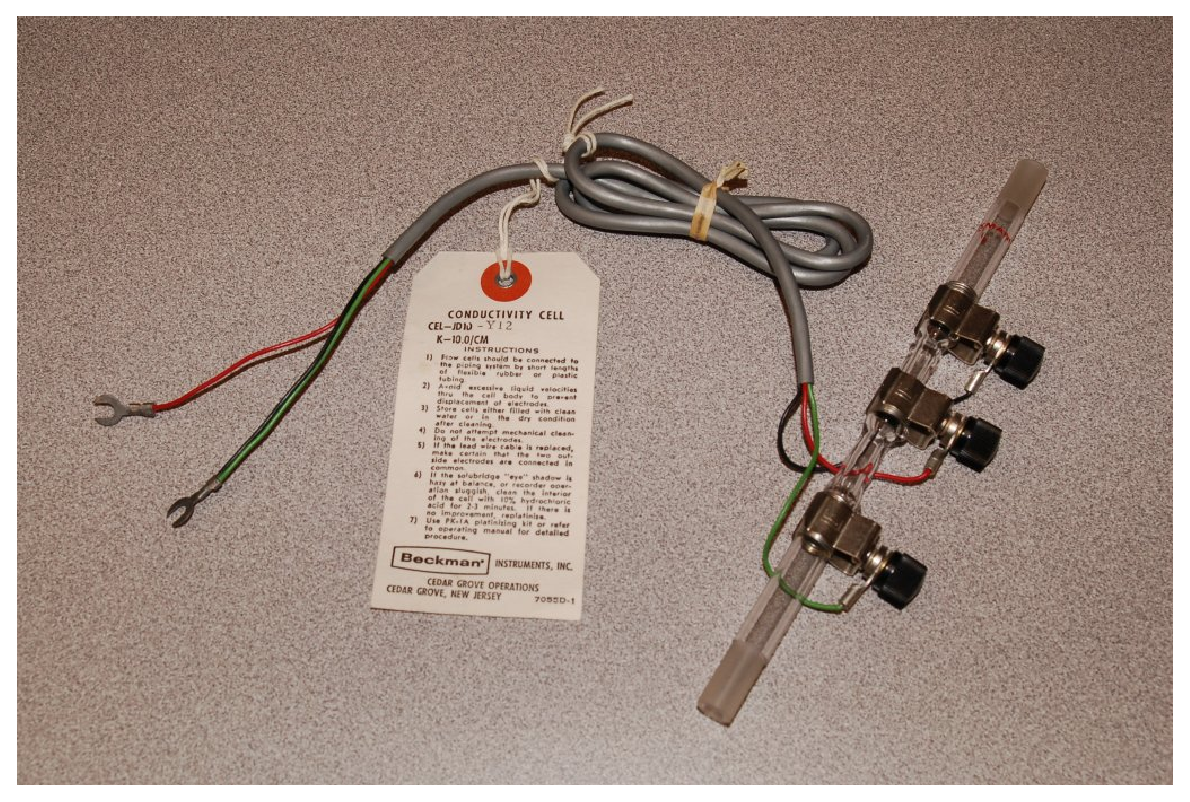
\includegraphics[width=4in]{conductivity06.eps}$$

Two-electrode conductivity cells are not very practical in real applications, because mineral and metal ions attracted to the electrodes tend to ``foul'' the electrodes over time forming solid, insulating barriers on the electrodes.  While this ``electroplating'' action may be substantially reduced by using AC instead of DC\footnote{The use of alternating current forces the ions to switch directions of travel many times per second, thus reducing the chance they have of bonding to the metal electrodes.} to excite the sensing circuit, it is usually not enough.  Over time, the conductive barriers formed by ions bonded to the electrode surfaces will create calibration errors by making the instrument ``think'' the liquid is less conductive than it actually is.






\filbreak
\subsection{Four-electrode conductivity probes}

A very old electrical technique known as the \textit{Kelvin} or \textit{four-wire} resistance-measuring method is a practical solution to the problem of electrode fouling faced by two-electrode conductivity probes.  Commonly employed to make precise resistance measurements for scientific experiments in laboratory conditions, as well as measuring the electrical resistance of strain gauges and other resistive sensors such as RTDs, the four-wire technique uses four conductors to connect the resistance under test to the measuring instrument: \index{Kelvin resistance measurement} \index{4-wire resistance measurement circuit}

$$\includegraphics{kelvin_4wire_01.eps}$$

Only the outer two conductors carry substantial current.  The inner two conductors connecting the voltmeter to the test specimen carry negligible current (due to the voltmeter's extremely high input impedance) and therefore drop negligible voltage along their lengths.  Voltage dropped across the current-carrying (outer) wires is irrelevant, since that voltage drop is never detected by the voltmeter.

Since the voltmeter only measures voltage dropped across the specimen (the resistor under test), and not the test resistance plus wiring resistance, the resulting resistance measurement is much more accurate than if only two wires were used to connect the test meters to the specimen.  

\filbreak

In the case of conductivity measurement, it is not wire resistance that we care to ignore, but rather the added resistance caused by fouling of the electrodes.  By using four electrodes instead of two, we are able to measure voltage dropped across a length of liquid solution \textit{only}, and completely ignore the resistive effects of electrode fouling:

$$\includegraphics{conductivity02.eps}$$

In the 4-wire conductivity cell, any electrode fouling will merely burden the current source by causing it to output a greater voltage, but it will \textit{not} affect the amount of voltage detected by the two inner electrodes as that electric current passes through the liquid.  Any fouling that happens to occur\footnote{There will be very little if any fouling on these electrodes anyway because they carry no current, and thus provide no reason for ions to migrate toward them.} on the two inner electrodes is of no effect to our conductivity measurement because these inner electrodes carry negligible current.  With little or no current through the inner electrodes, there will be negligible voltage dropped across any resistive coating that happens to form on them, and thus the voltmeter will still register the true voltage dropped by the liquid solution.

If the solution's conductivity is defined as the product of the measured conductance and the cell constant ($k = G \theta$), and conductance is defined as the ratio of current to voltage ($G = {I \over V}$), then we may determine conductivity from voltage and current measurements by combining these two equations:

$$k = G \theta \hskip 30pt G = {I \over V}$$

$$\hbox{\textit{. . . substituting} } {I \over V} \hbox{\textit{ for }} G \hbox{\textit{ . . .}}$$

$$k = {I \over V} \theta \hskip 15pt \hbox{or} \hskip 15pt k = {{I \theta} \over V}$$


\filbreak

Some conductivity instruments employ a second voltmeter to measure the voltage dropped between the ``excitation'' electrodes, to indicate electrode fouling:

$$\includegraphics{conductivity03.eps}$$

Any form of electrode fouling will cause this secondary voltage measurement to disproportionately exceed the first, thus providing an indicator that instrument technicians may use for predictive maintenance (telling them when the probes need cleaning or replacement).  Meanwhile, the primary voltmeter will do its job of accurately measuring liquid conductivity so long as the current source is still able to output its normal amount of current.






\filbreak
\subsection{Electrodeless conductivity probes}

An entirely different design of conductivity cell called \textit{electrodeless} uses electromagnetic induction rather than direct electrical contact to detect the conductivity of the liquid solution.  This cell design enjoys the distinct advantage of virtual immunity to fouling\footnote{Toroidal conductivity sensors may suffer calibration errors if the fouling is so bad that the hole becomes choked off with sludge, but this is an extreme condition.  These sensors are far more tolerant to fouling than any form of contact-type (electrode) conductivity cell.}, since there is no direct electrical contact between the measurement circuit and the liquid solution.  Instead of using two or four electrodes inserted into the solution for conductivity measurement, this cell uses two \textit{toroidal} inductors (one to induce an AC voltage in the liquid solution, and the other to measure the strength of the resulting current through the solution):  \index{Electrodeless conductivity cell}  \index{Toroidal conductivity cell}

$$\includegraphics{conductivity04.eps}$$

The basic idea of this instrument is that a primary coil energized by AC power induces an electric current that passes through the sample liquid.  This current, in turn, induces a measurable voltage in a secondary coil.  Since ferromagnetic toroids do an excellent job of containing their own magnetic fields, there will be negligible mutual inductance between the two wire coils.  The \textit{only} way a voltage will be induced in the secondary coil is if there is an AC current passing through the center of that coil, through the liquid itself.  If the liquid is non-conductive, the secondary coil will see no induced voltage at all despite being situated near the energized primary coil.  The more conductive the liquid solution, the more current will pass through the center of both coils (through the liquid), thus producing a greater induced voltage at the secondary coil.  Secondary coil voltage therefore is directly proportional to liquid conductivity\footnote{Note that this is opposite the behavior of a direct-contact conductivity cell, which produces \textit{less} voltage as the liquid becomes more conductive.}.

\filbreak

The equivalent electrical circuit for a toroidal conductivity probe looks like a pair of transformers, with the liquid acting as a resistive path for current to connect the two transformers together:

$$\includegraphics{conductivity05.eps}$$

\vskip 10pt

Toroidal conductivity cells are preferred over direct-contact conductivity cells whenever possible, due to their ruggedness and virtual immunity to fouling.  However, toroidal cells are not sensitive enough for conductivity measurement in high-purity applications such as boiler feedwater treatment and ultra-pure water treatment necessary for pharmaceutical and semiconductor manufacturing.  As always, the manufacturer's specifications are the best source of information for conductivity cell applicability in any particular process.

The following photograph shows a toroidal conductivity probe mounted on a display board at a trade-show, along with a conductivity transmitter (to both display the conductivity measurement in millisiemens per centimeter and also transmit the measurement as a 4-20 mA analog signal):

$$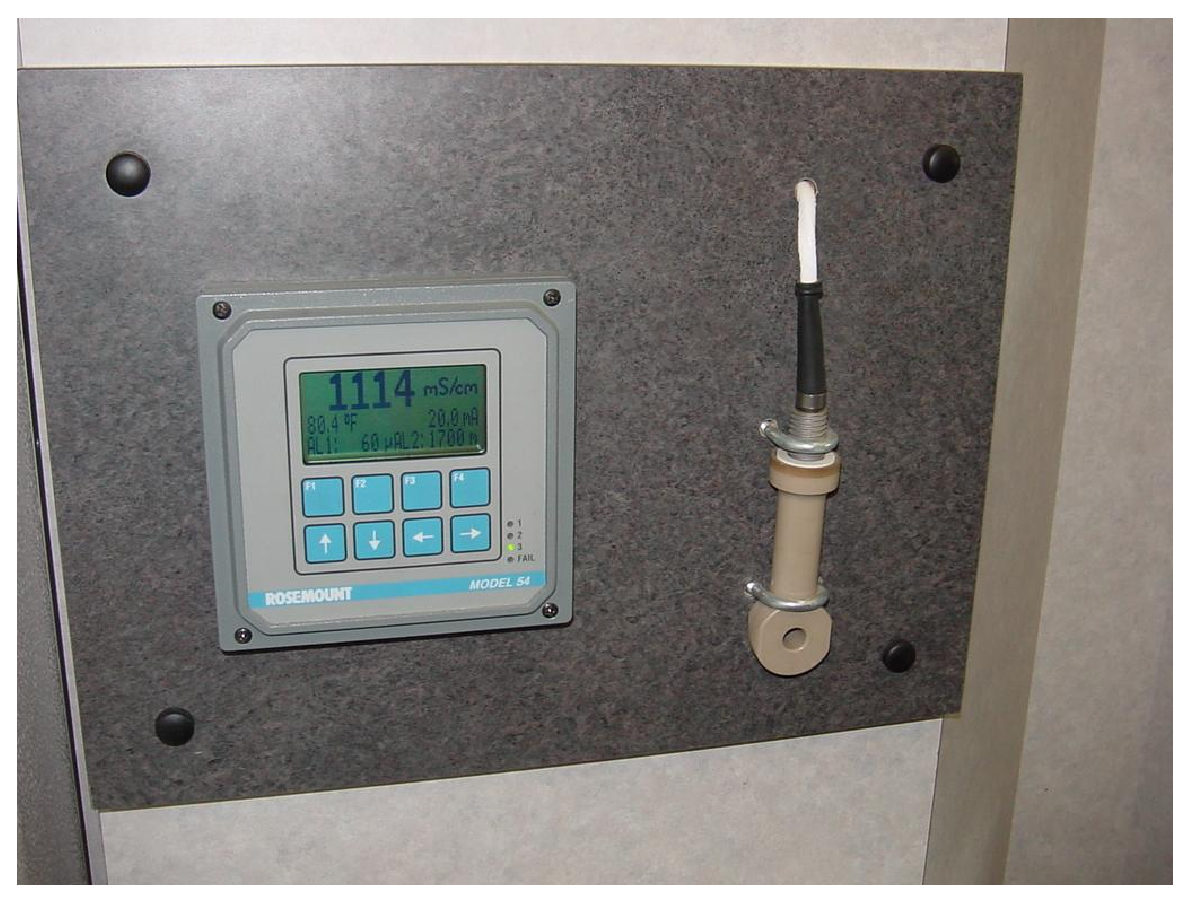
\includegraphics[width=5in]{Rosemount_conductivity_analyzer.eps}$$








\filbreak
\section{pH measurement}

\label{pH_measurement}

pH is the measurement of the hydrogen ion activity in a liquid solution.  It is one of the most common forms of analytical measurement in industry, because pH has a great effect on the outcome of many chemical processes.  Food processing, water treatment, pharmaceutical production, steam generation (thermal power plants), and alcohol manufacturing are just some of the industries making extensive use of pH measurement (and control).  pH is also a significant factor in the corrosion of metal pipes and vessels carrying aqueous (water-based) solutions, so pH measurement and control is important in the life-extension of these capital investments.

In order to understand pH measurement, you must first understand the chemistry of pH.  Please refer to section \ref{pH} beginning on page \pageref{pH} for a theoretical introduction to pH.






\filbreak
\subsection{Colorimetric pH measurement}

One of the simplest ways to measure the pH of a solution is by color.  Some chemical compounds dissolved in an aqueous solution will change color if the pH value of that solution falls within a certain range.  \textit{Litmus paper} is a common laboratory application of this principle, where a color-changing chemical substance infused on a paper strip changes color when dipped in the solution.  Comparing the final color of the litmus paper to a reference chart yields an approximate pH value for the solution.

A natural example of this phenomenon is well-know to flower gardeners, who recognize that hydrangea blossoms change color with the pH value of the soil.  In essence, these plants act as organic litmus indicators\footnote{Truth be told, the color of a hydrangea blossom is only indirectly determined by soil pH.  Soil pH affects the plant's uptake of aluminum, which is the direct cause of color change.  Interestingly, the pH-color relationship of a hydrangea plant is exactly opposite that of common laboratory litmus paper: red litmus paper indicates an acidic solution while blue litmus paper indicates an alkaline solution; whereas red hydrangea blossoms indicate alkaline soil while blue (or violet) hydrangea blossoms indicate acidic soil.}.  This hydrangea plant indicates acidic soil by the violet color of its blossoms:

$$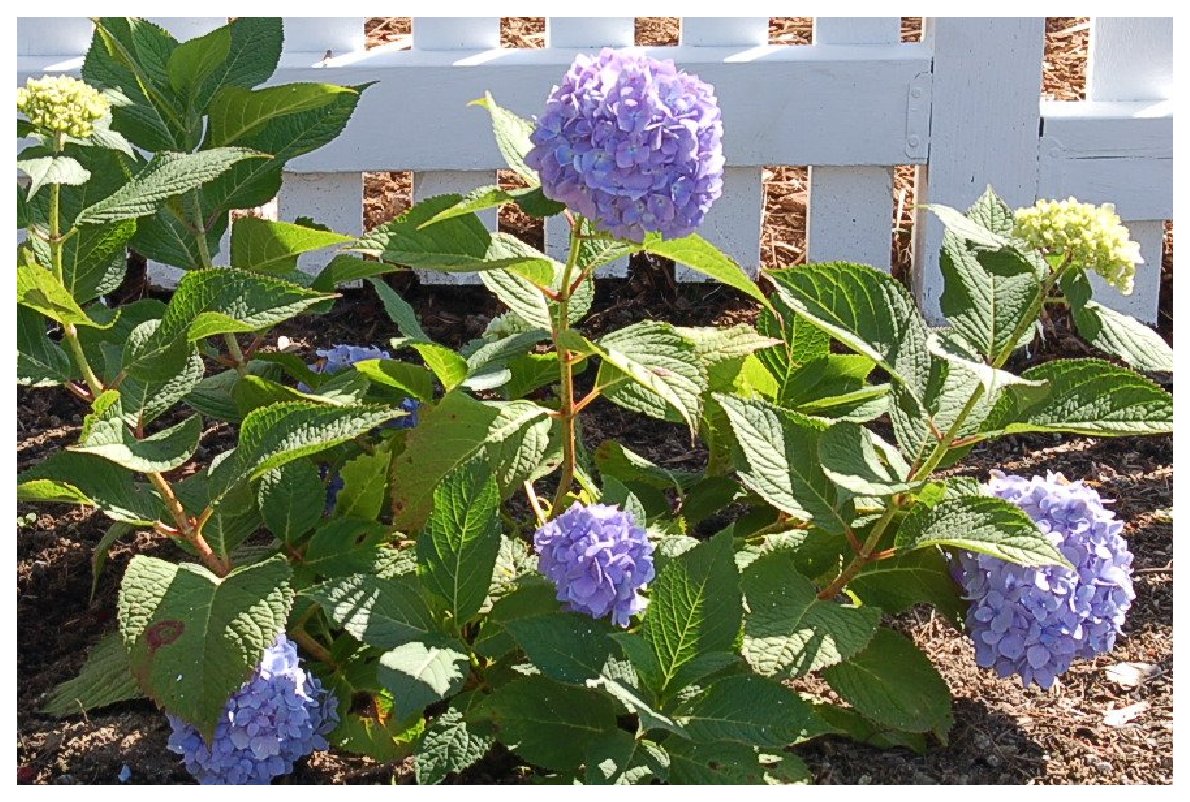
\includegraphics[width=4in]{ph_02.eps}$$

\filbreak

Another example of a natural colorimetric pH indicator is \textit{red cabbage}.  If some red cabbage is chopped and cooked, the juices released by the cabbage\footnote{\textit{Flavin}, classified as an \textit{anthocyanin}, is the pigment in red cabbage responsible for the pH-indicating behavior.  This same pigment also changes color according to soil pH while the cabbage plant is growing, much like a hydrangea.  Unlike hydrangeas, the coloring of a red cabbage is more akin to litmus paper, with red indicating acidic soil.} will be sensitive to pH.  This makes a very easy demonstration for the home kitchen.  In these two photographs, you see how liquid may be collected from the cabbage in a steaming pot, and then transferred to three glasses for testing:

$$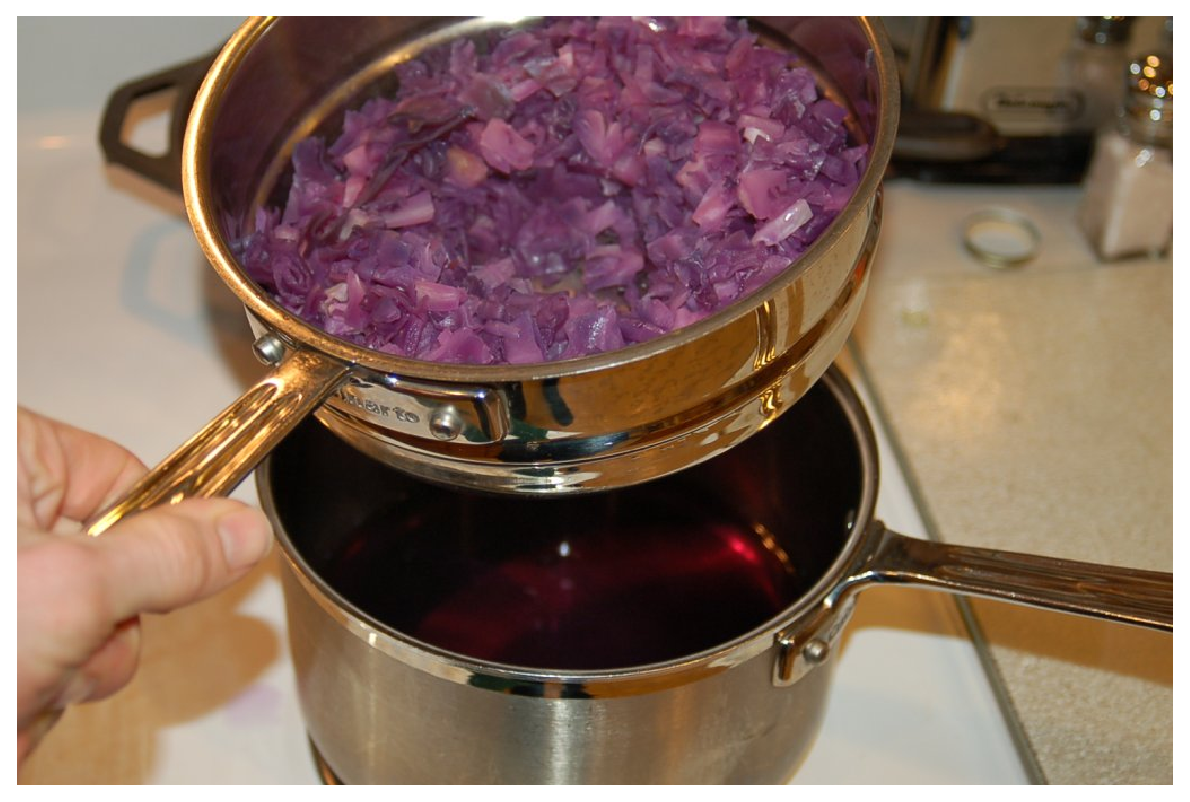
\includegraphics[width=2.5in]{ph_19.eps} \hskip 50pt 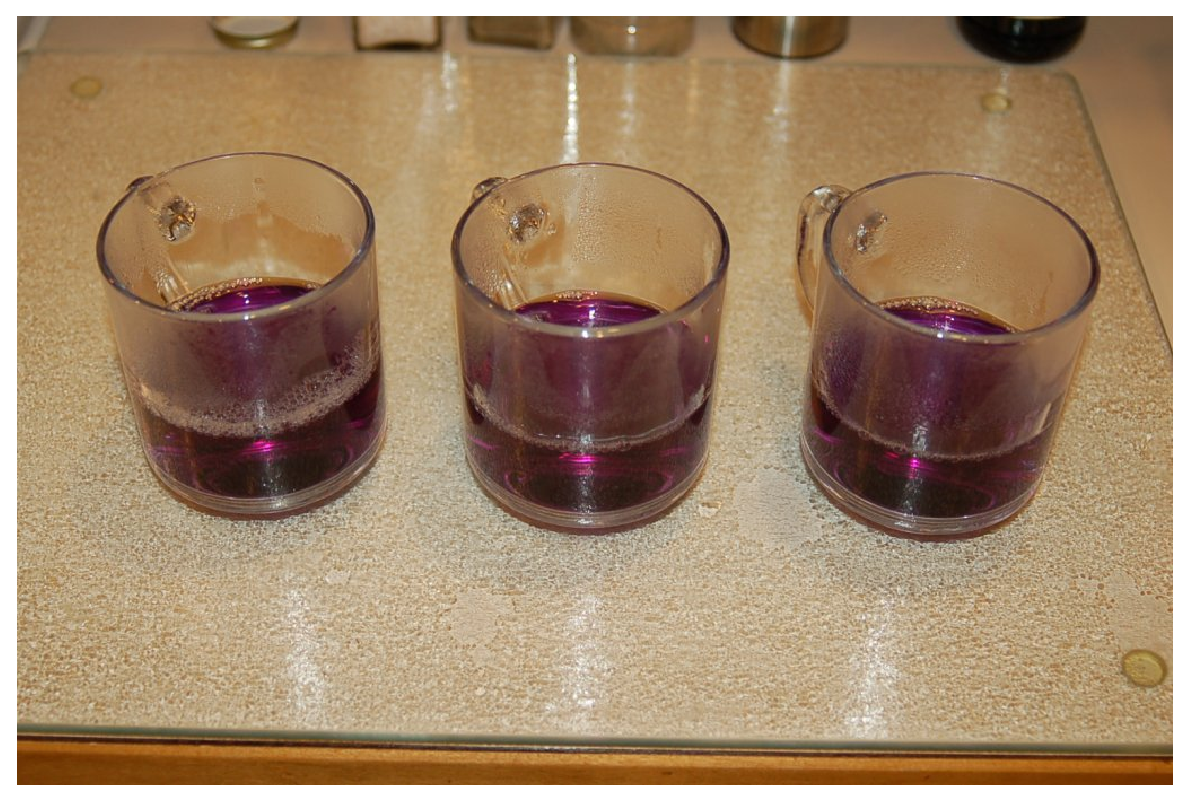
\includegraphics[width=2.5in]{ph_20.eps}$$

Adding vinegar (acid) to one glass, baking soda (caustic/base/alkaline) to another glass, and leaving the third glass unaltered (as an experimental ``control''), we see striking differences in the color of each solution.  Vinegar turns the cabbage juice red, while baking soda turns it dark green, compared to its original purple color:

$$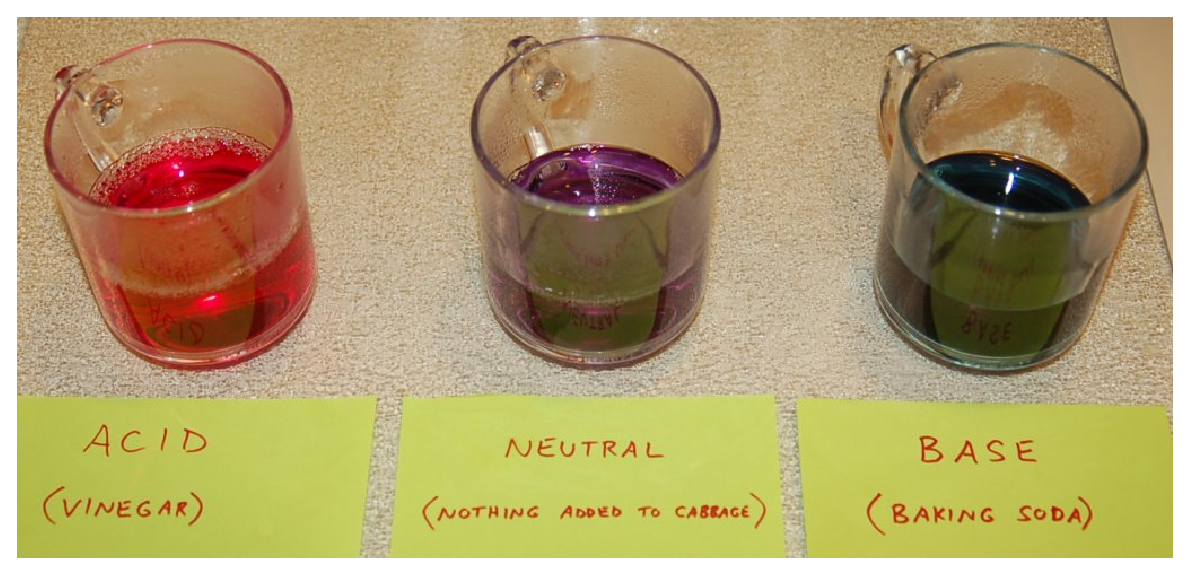
\includegraphics[width=6in]{ph_21.eps}$$

In fact, you may make your own crude form of litmus paper by soaking paper strips with red cabbage juice!










\filbreak
\subsection{Potentiometric pH measurement}

Color-change is a common pH test method used for manual laboratory analyses, but it is not well-suited to continuous process measurement.  By far the most common pH measurement method in use is \textit{electrochemical}: special pH-sensitive electrodes inserted into an aqueous solution will generate a voltage dependent upon the pH value of that solution.

Like all other potentiometric (voltage-based) analytical measurements, electrochemical pH measurement is based on the \textit{Nernst equation}, which describes the electrical potential created by ions migrating through a permeable membrane.  The ``textbook example'' of this is a device called a \textit{concentration cell}, where two halves of an electrochemical cell are filled with solutions having different concentrations of ions (i.e. different molarities): \index{Nernst equation}  \index{Concentration cell}

$$\includegraphics{ph_17.eps}$$

\noindent
Where,

$V$ = Voltage produced across membrane due to ion exchange (volts)

$R$ = Universal gas constant (8.315 J/mol$\cdot$K)

$T$ = Absolute temperature (Kelvin)

$n$ = Number of electrons transferred per ion exchanged (unitless)

$F$ = Faraday constant, in coulombs per mole (96485 C/mol e$^{-}$)

$C_1$ = Concentration of ion in measured solution (moles per liter of solution, $M$)

$C_2$ = Concentration of ion in reference solution (moles per liter of solution, $M$)

\vskip 10pt

As ions naturally migrate through this membrane in an attempt\footnote{Of course, ions possess no agency and therefore cannot literally ``attempt'' anything.  What is happening here is the normal process of \textit{diffusion} whereby the random motions of individual molecules tends to evenly distribute those molecules throughout a space.  If a membrane divides two solutions of differing ionic concentration, ions from the more concentrated region will, over time, migrate to the region of lower concentration until the two concentrations are equal to each other.  Truth be told, ions are continually migrating in \textit{both} directions through the porous membrane at all times, but the rate of migration from the high concentration to the low concentration solutions is greater than the other direction simply because there are more ions present to migrate that way.  After the two solutions have become equal in ionic concentration, the random migration still proceeds in both directions, but now the rates in either direction are equal and therefore there is zero \textit{net} migration.} to equalize the two concentrations, a voltage corresponding to the \textit{difference} in ion concentrations between the two cell halves will develop between the two electrodes.  The greater the difference in concentrations between the two sides, the greater the voltage produced by the cell.  The Nernst voltage may be used to infer the concentration of a specific type of ion if the membrane is \textit{selectively permeable} to that one type of ion.  \index{Selective permeability}

We may write the Nernst equation using either natural logarithms ($\ln$) or common logarithms ($\log$).  Either form of the Nernst equation works to predict the voltage generated by a concentration cell.  The typical form applied to pH measurement calculations is the common log version, which makes more intuitive sense since pH is defined as the common logarithm of hydrogen ion activity:

$$V = {{R T} \over {nF}} \ln \left({C_1 \over C_2}\right) \hskip 50pt V = {{2.303 R T} \over {nF}} \log \left({C_1 \over C_2}\right)$$

Both forms of the Nernst equation predict a greater voltage developed across the thickness of a membrane as the concentrations on either side of the membrane differ to a greater degree.  If the ionic concentration on both sides of the membrane are equal, no Nernst potential will develop\footnote{This is apparent from a mathematical perspective by examination of the Nernst equation: if the concentrations are equal (i.e. $C_1 = C_2$), then the ratio of $C_1 \over C_2$ will be equal to 1.  Since the logarithm of 1 is zero, this predicts zero voltage generated across the membrane.  From a chemical perspective, this corresponds to the condition where random ion migration through the porous membrane is equal in both directions.  In this condition, the Nernst potentials generated by the randomly-migrating ions are equal in magnitude and opposite in direction (polarity), and therefore the membrane generates zero overall voltage.}.

\filbreak

In the case of pH measurement, the Nernst equation describes the amount of electrical voltage developed across a special \textit{glass} membrane due to hydrogen ion exchange between the process liquid solution and a \textit{buffer solution} inside the bulb formulated to maintain a constant pH value of 7.0 pH.  Special pH-measurement electrodes are manufactured with a closed end made of this glass, a small quantity of buffer solution contained within the glass bulb:  \index{Measurement electrode}  \index{Buffer solution}

$$\includegraphics{ph_03.eps}$$

Any concentration of hydrogen ions in the process solution differing from the hydrogen ion concentration in the buffer solution ([H$^{+}$] = 1 $\times$ 10$^{-7}$ $M$) will cause a voltage to develop across the thickness of the glass.  Thus, a standard pH measurement electrode produces no potential when the process solution's pH value is exactly 7.0 pH (i.e. when the process solution has the same hydrogen ion activity as the buffer solution within the bulb).

Given the knowledge that the measurement bulb is filled with a buffer solution having a pH value of 7, we may conclude that one of the concentrations for the glass membrane will always have a value of $1 \times 10^{-7} \> M$.  We may manipulate the Nernst equation to reflect this knowledge, and to express the potential developed in terms of the pH of both solutions, since we know pH is defined the negative logarithm of hydrogen ion molarity:

$$V = {{2.303 R T} \over {nF}} \log \left({C_1 \over C_2}\right)$$

$$V = {{2.303 R T} \over {nF}} \left( \log C_1 - \log C_2 \right)$$

$$\hbox{If we know that pH} = -\log [\hbox{H}^{+}]$$

$$V = {{2.303 R T} \over {nF}} \left(- \hbox{pH}_1 - (- \hbox{pH}_2) \right)$$

$$V = {{2.303 R T} \over {nF}} \left(\hbox{pH}_2 - \hbox{pH}_1 \right)$$

$$V = {{2.303 R T} \over {nF}} \left(7 - \hbox{pH}_1 \right)$$

Thus, the Nernst voltage produced by a glass pH electrode is directly proportional to the difference in pH value between the measured solution (pH$_{1}$) and the probe's internal 7.0 pH buffer.

\vskip 10pt

The glass used to manufacture this electrode is no ordinary glass.  Rather, it is specially manufactured to be \textit{selectively permeable} to hydrogen ions\footnote{It is a proven fact that sodium ions in relatively high concentration (compared to hydrogen ions) will also cause a Nernst potential across the glass of a pH electrode, as will certain other ion species such as potassium, lithium, and silver.  This effect is commonly referred to as \textit{sodium error}, and it is usually only seen at high pH values where the hydrogen ion concentration is extremely low.  Like any other analytical technology, pH measurement is subject to ``interference'' from species unrelated to the substance of interest.}.  If it were not for this fact, the electrode might generate voltage as it contacted any number of different ions in the solution.  This would make the electrode non-specific, and therefore useless for pH measurement.  \index{Sodium error, pH measurement}  \index{Species, chemical composition}

Manufacturing processes for pH-sensitive glass are highly guarded trade secrets.  There seems to be something of an art to the manufacture of an accurate, reliable, and long-lived pH electrode.  A variety of different measurement electrode designs exist for different process applications, including high pressure and high temperature services.

\filbreak

Actually measuring the voltage developed across the thickness of the glass electrode wall, however, presents a bit of a problem: while we have a convenient electrical connection to the solution \textit{inside} the glass bulb, we do not have any place to connect the other terminal of a sensitive voltmeter to the solution \textit{outside} the bulb\footnote{Remember that voltage is always measured \textit{between two points!}}.  In order to establish a complete circuit from the glass membrane to the voltmeter, we must create a zero-potential electrical junction with the process solution.  To do this, we use another special electrode called a \textit{reference electrode} immersed in the same liquid solution as the measurement electrode:  \index{Reference electrode}

$$\includegraphics{ph_04.eps}$$

\filbreak

Together, the measurement and reference electrodes provide a voltage-generating element sensitive to the pH value of whatever solution they are submerged in:

$$\includegraphics{ph_05.eps}$$

The most common configuration for modern pH probe sets is what is called a \textit{combination electrode}, which combines both the glass measurement electrode and the porous reference electrode in a single unit.  This photograph shows a typical industrial combination pH electrode:  \index{Combination electrode}

$$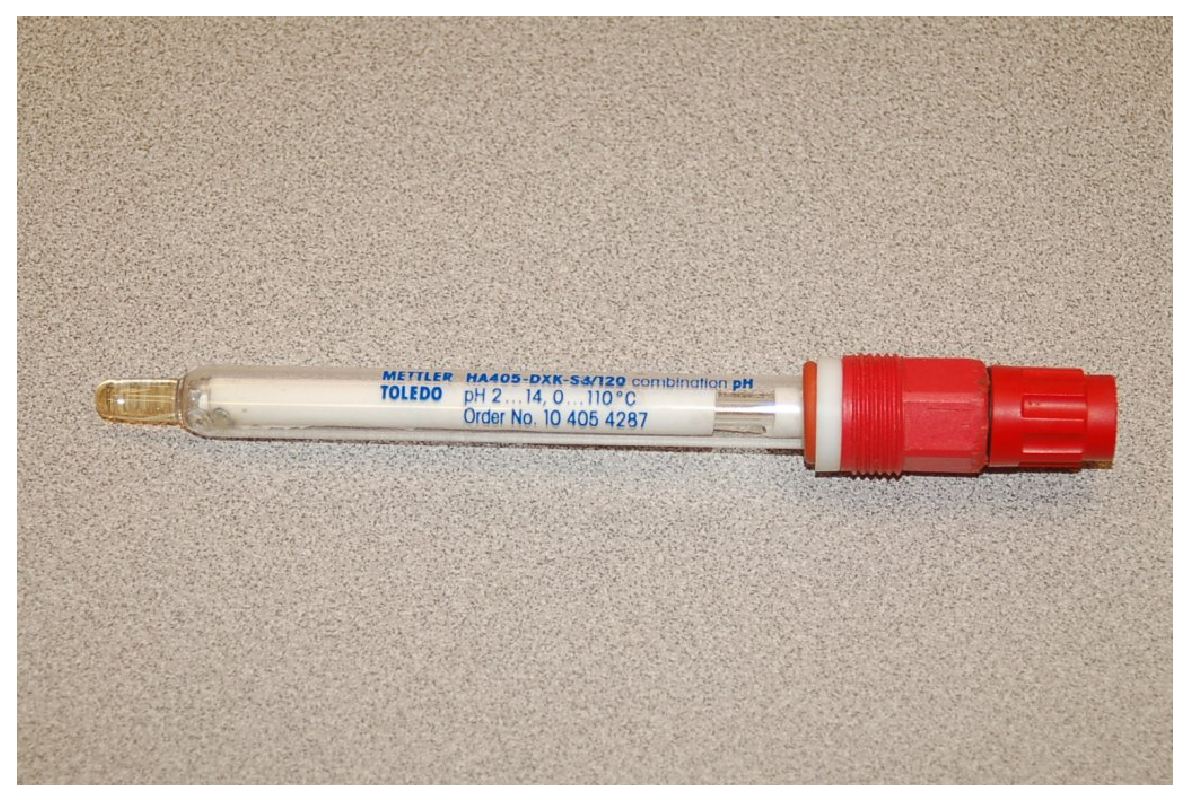
\includegraphics[width=5in]{phprobe.eps}$$

The red-colored plastic cap on the right-hand end of this combination electrode covers and protects a gold-plated coaxial electrical connector, to which the voltage-sensitive pH indicator (or transmitter) attaches.

Another model of pH probe appears in the next photograph.  Here, there is no protective plastic cap covering the probe connector, allowing a view of the gold-plated connector bars:

$$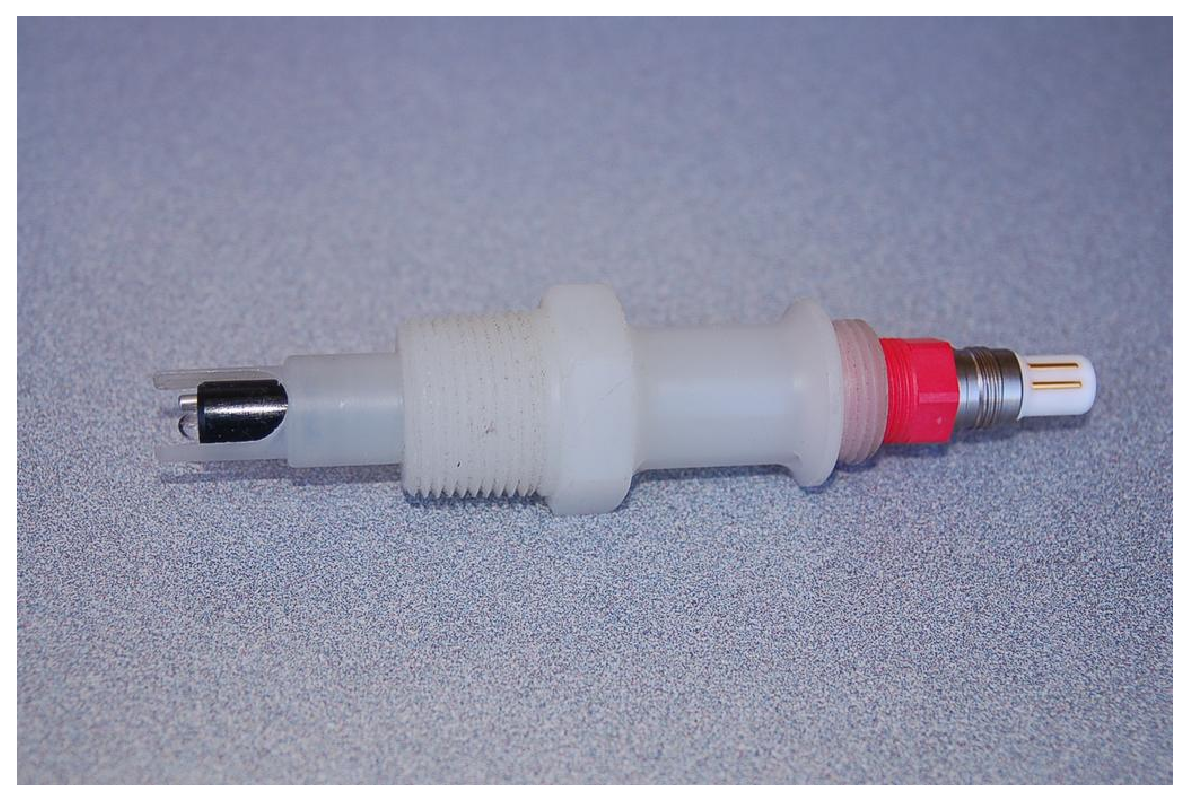
\includegraphics[width=5in]{phprobe2.eps}$$

\filbreak

A close-up photograph of the probe tip reveals the glass measurement bulb, a weep hole for process liquid to enter the reference electrode assembly (internal to the white plastic probe body), and a metal \textit{solution ground} electrode:

$$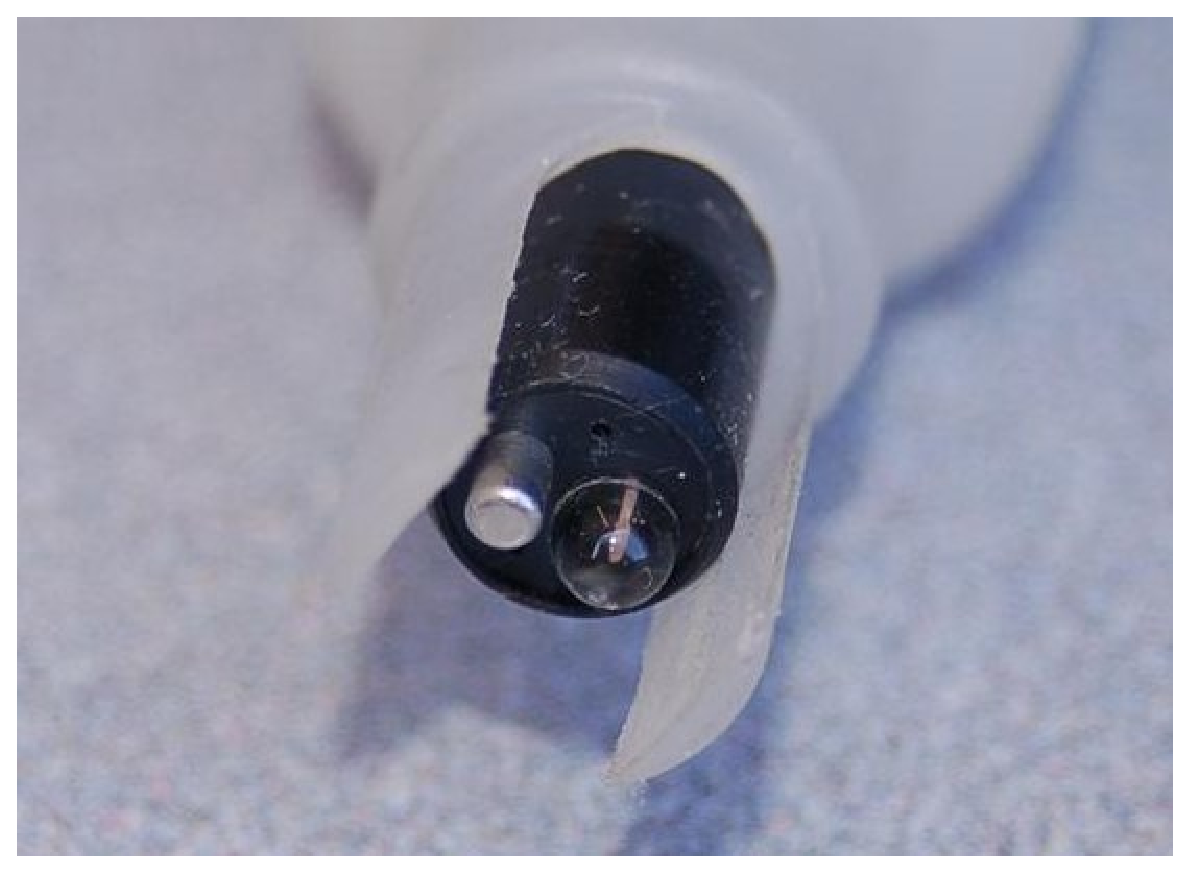
\includegraphics[width=5in]{phprobe3.eps}$$

It is extremely important to always keep the glass electrode wet.  Its proper operation depends on complete \textit{hydration} of the glass, which allows hydrogen ions to penetrate the glass and develop the Nernst potential.  The probes shown in these photographs are shown in a dry state only because they have already exhausted their useful lives and cannot be damaged any further by dehydration.  \index{Hydration, pH electrode}

The process of hydration -- so essential to the working of the glass electrode -- is also a mechanism of wear for pH probes.  Layers of glass ``slough'' off over time when continuously hydrated, which means that glass pH electrodes have a limited life whether they are being used to measure the pH of a process solution (continuously wet) or if they are being stored on a shelf (maintained in a wet state by a small quantity of potassium hydroxide held close to the glass probe by a liquid-tight cap).  It is therefore impossible to extend the shelf life of a glass pH electrode indefinitely. \index{Shelf life, pH electrode}

\vskip 10pt

\filbreak

A common installation for industrial pH probe assemblies is to simply dip them into an open vessel containing the solution of interest.  This arrangement is very common in water treatment applications, where the water mostly flows in open vessels by gravity at the treatment facility.  A photograph showing a pH measurement system for the ``outfall'' flow of water from an industrial facility appears here:

$$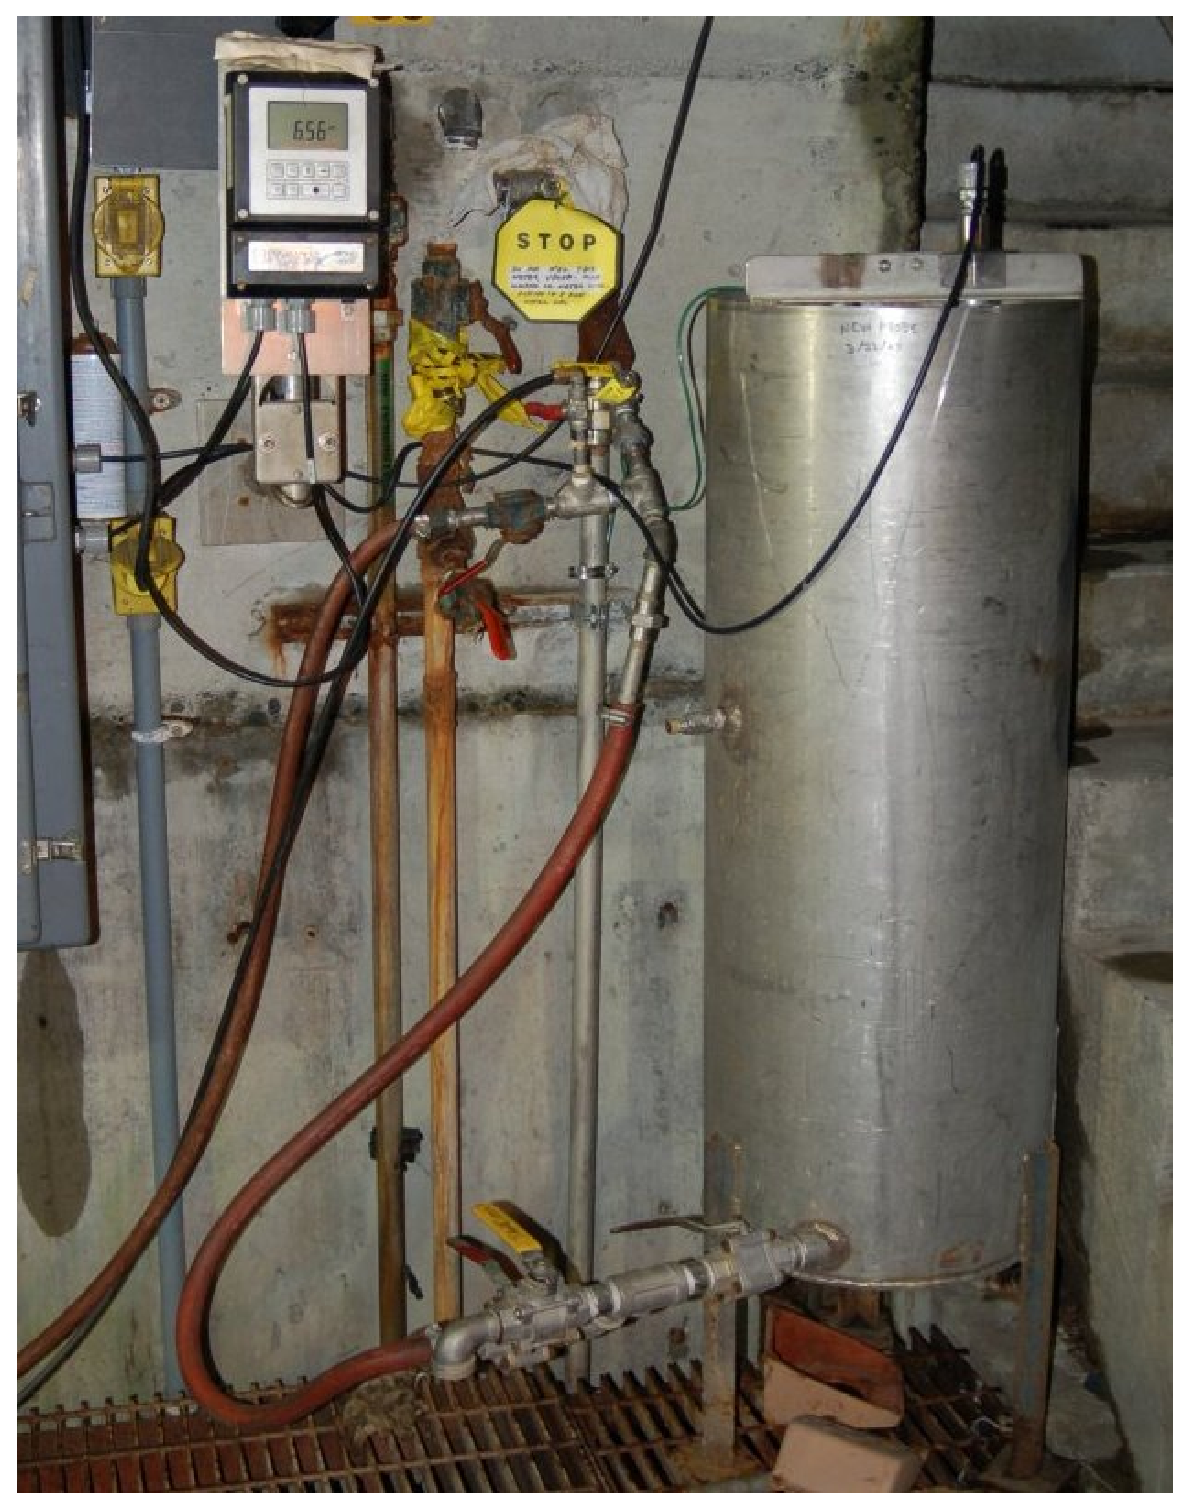
\includegraphics[height=6in]{ph_11.eps}$$

\filbreak

Water flowing from the discharge pipe of the facility enters an open-top stainless steel tank where the pH probe hangs from a bracket.  An overflow pipe maintains a maximum water level in the tank as water continuously enters it from the discharge pipe.  The probe assembly may be easily removed for maintenance:

$$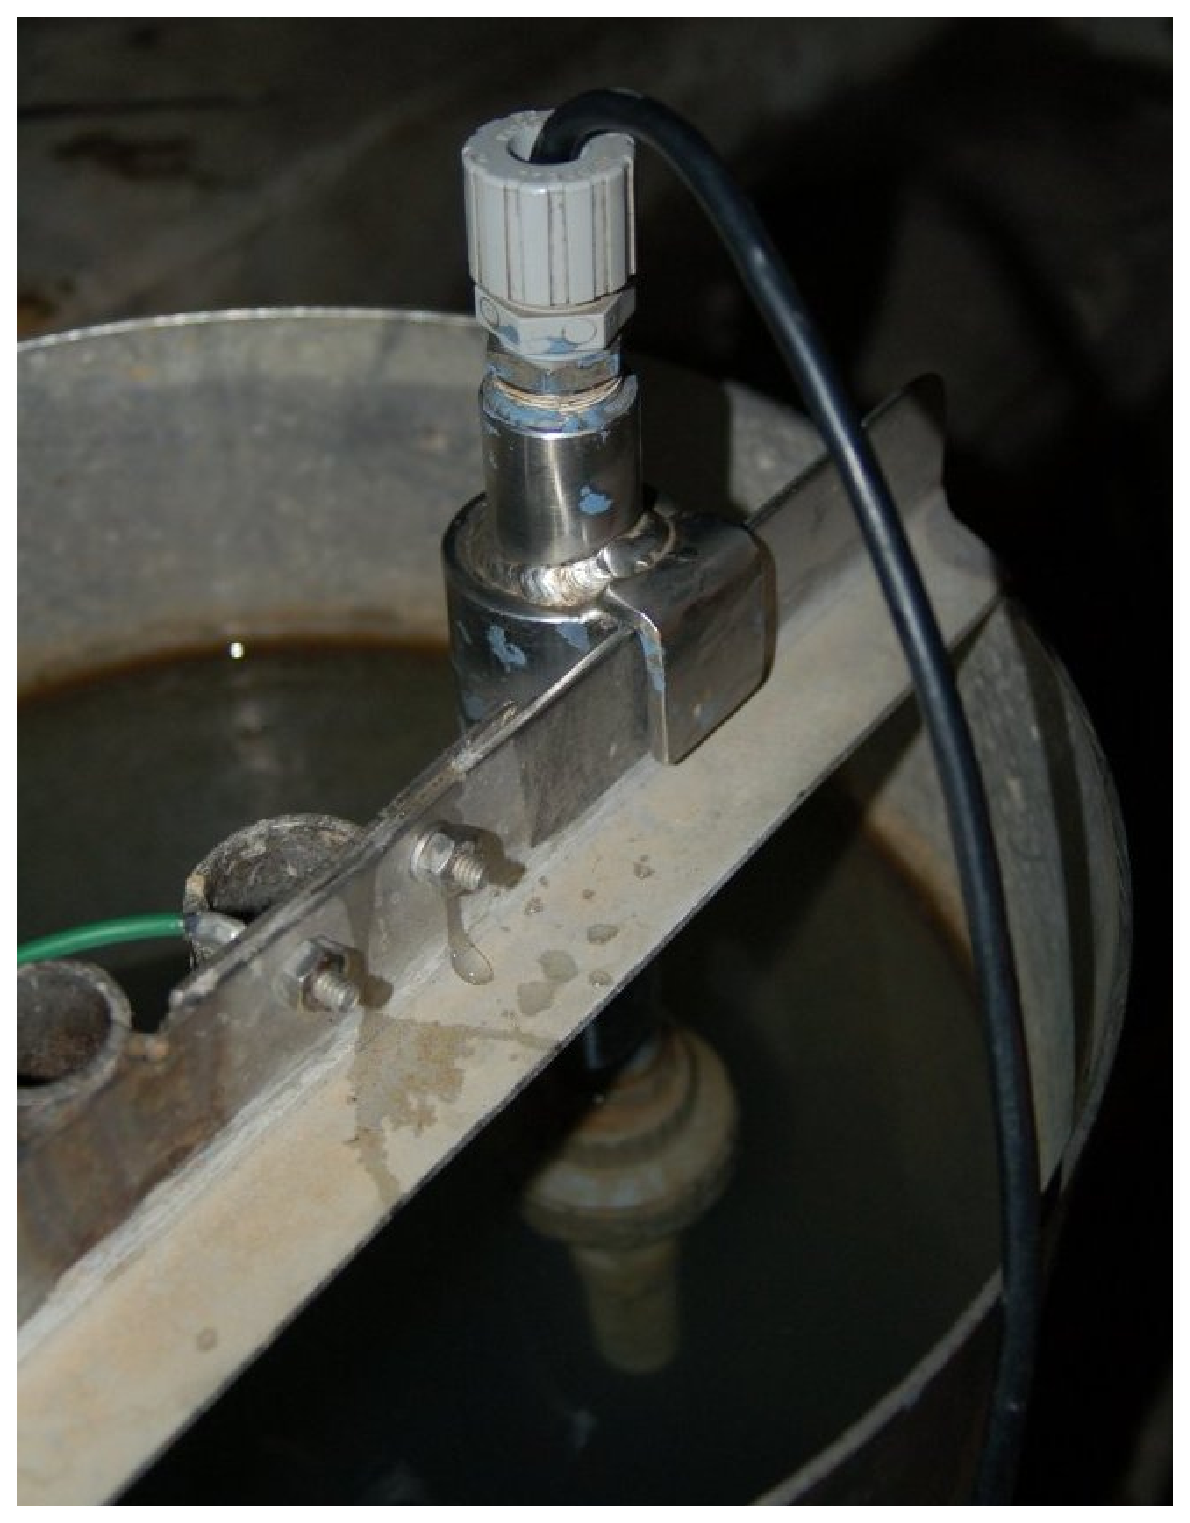
\includegraphics[height=3in]{ph_12.eps} \hskip 50pt 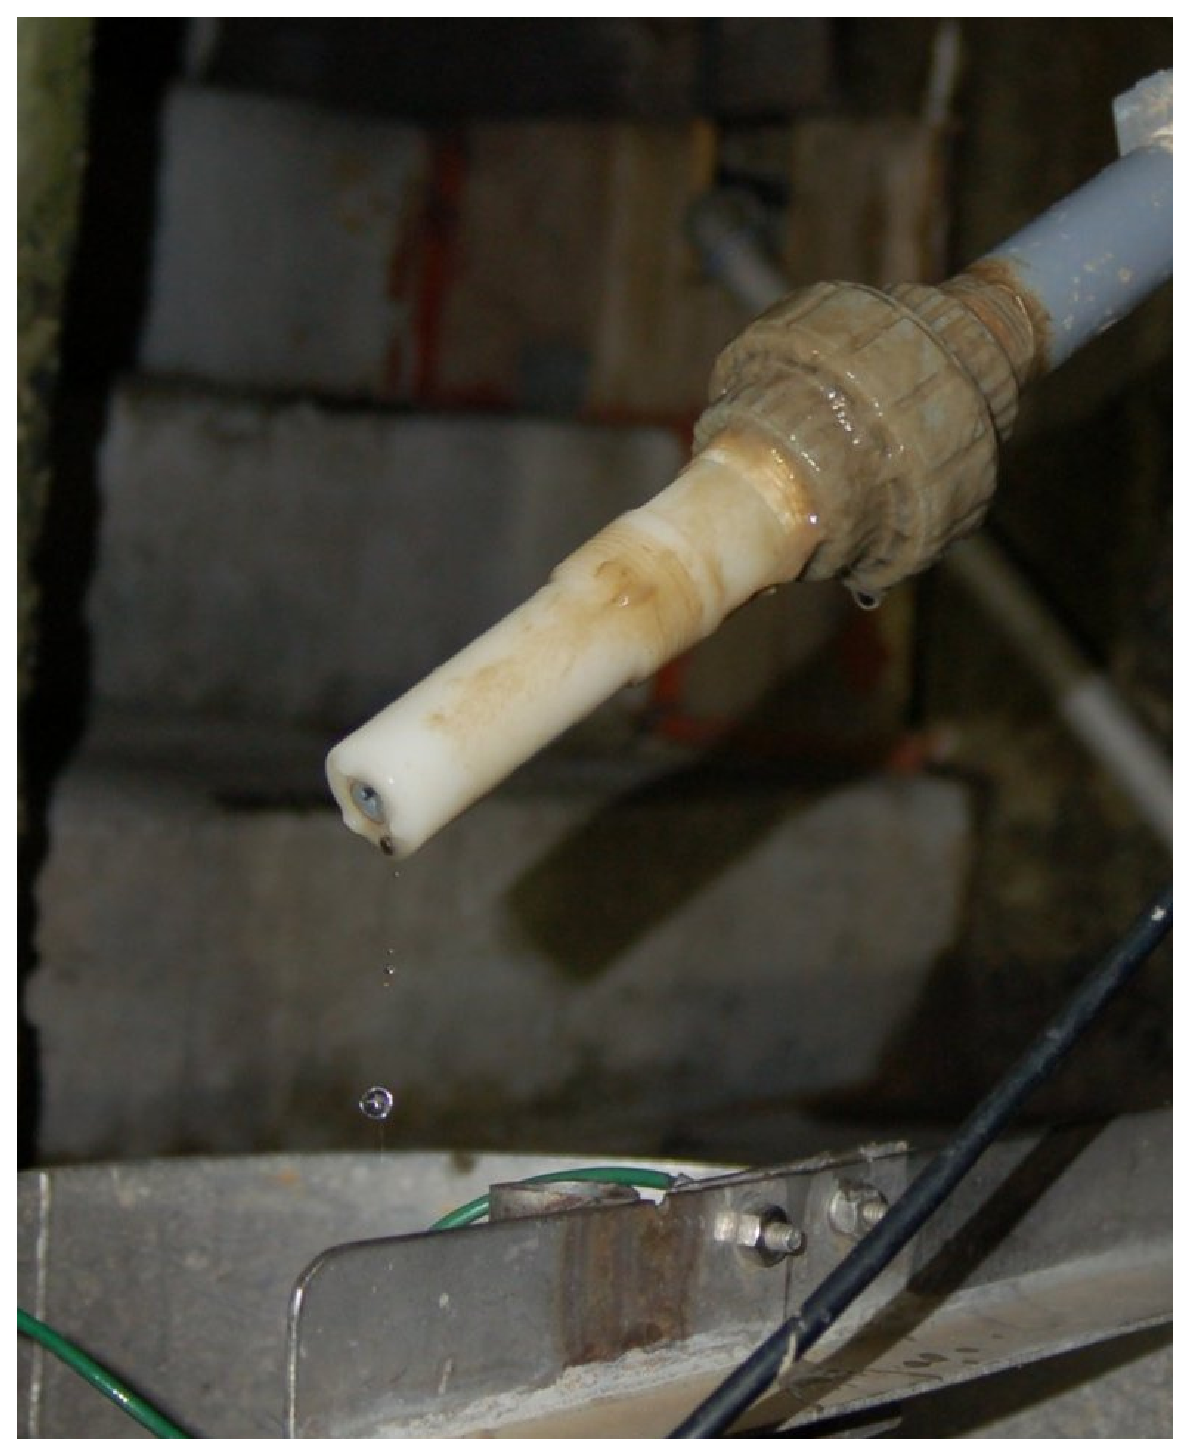
\includegraphics[height=3in]{ph_13.eps}$$

\filbreak

An alternative design for industrial pH probes is the \textit{insertion} style, designed to install in a pressurized pipe.  Insertion probes are designed to be removed while the process line remains pressurized, to facilitate maintenance without interrupting continuous operation:

$$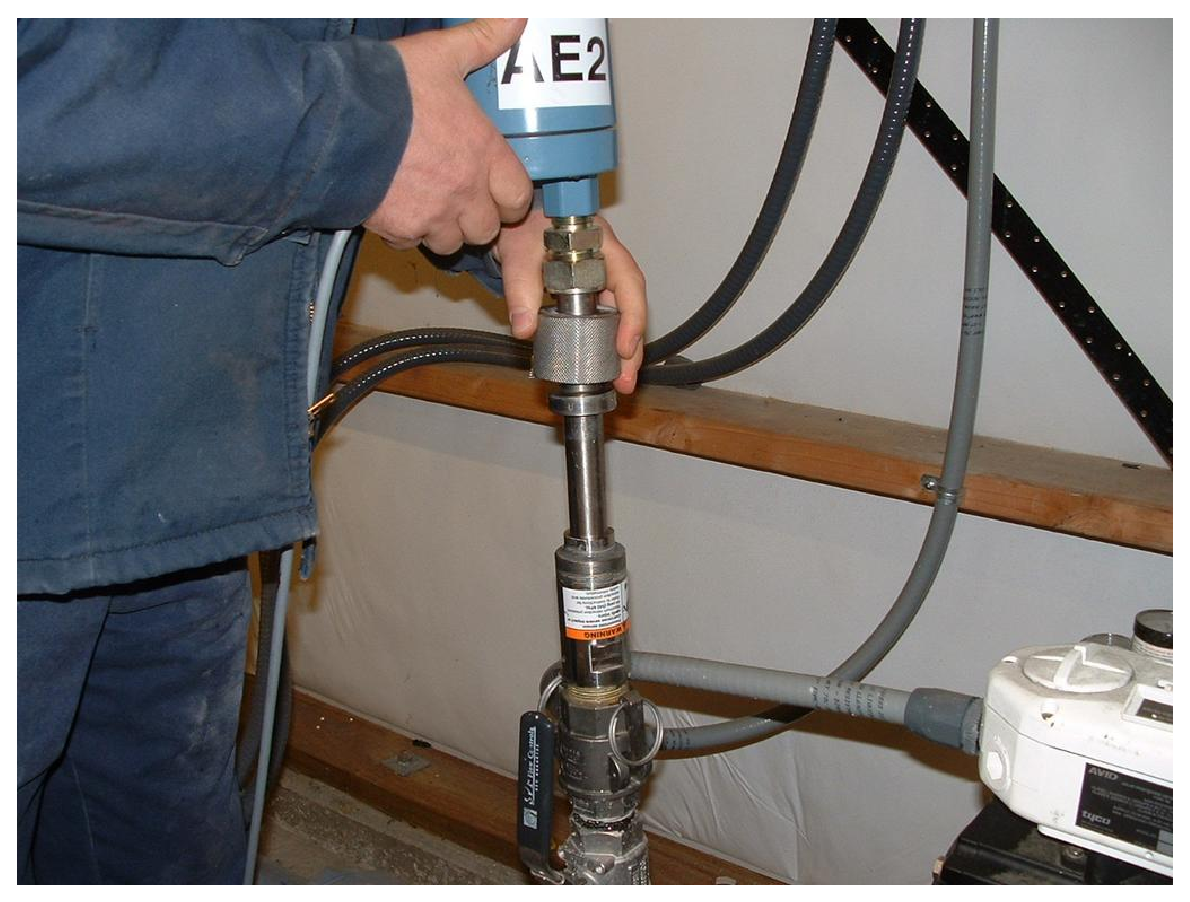
\includegraphics[width=2.5in]{ph_15.eps} \hskip 50pt 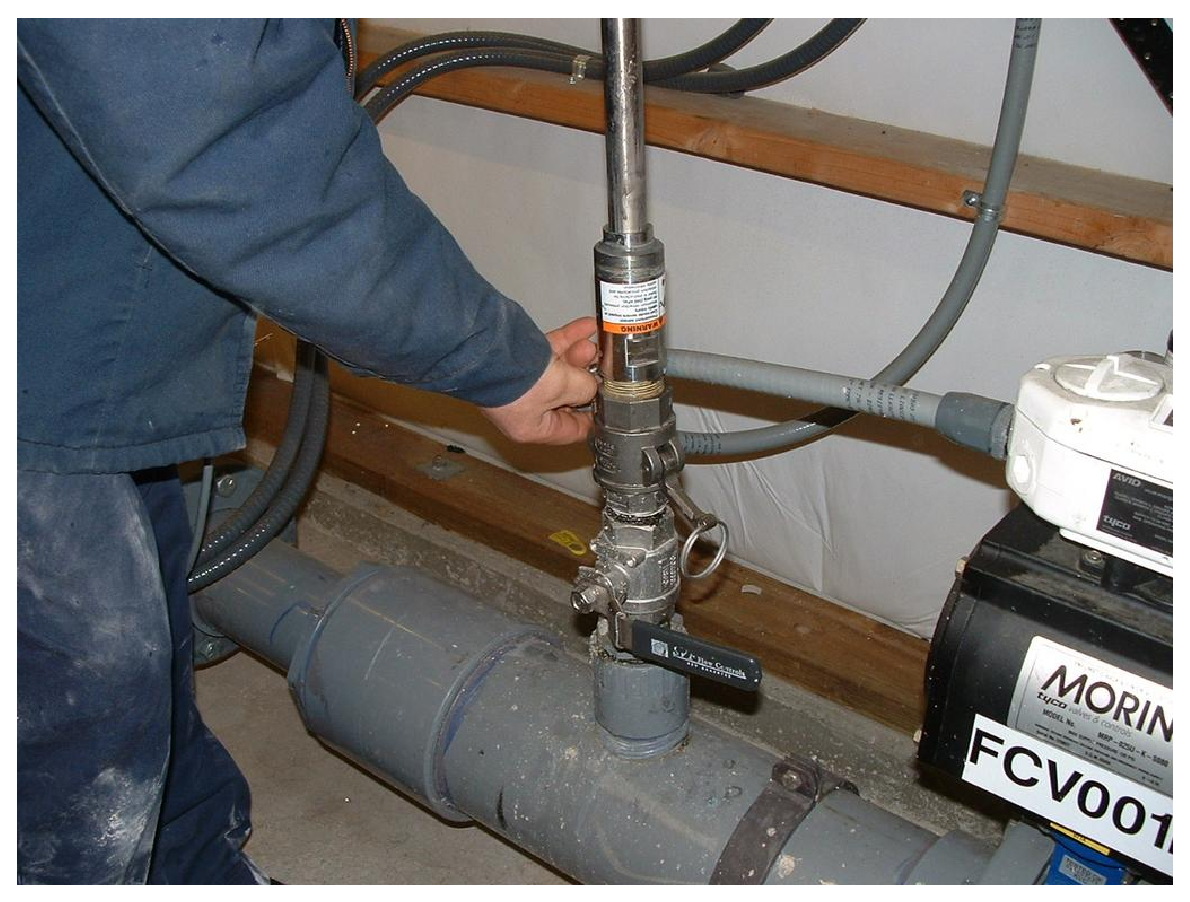
\includegraphics[width=2.5in]{ph_16.eps}$$

The probe assembly inserts into the process line through the open bore of a 90$^{o}$ turn ball valve.  The left-hand photograph (above) shows the retaining nut loosened, allowing the probe to slide up and out of the pipe.  The right-hand photograph shows the ball valve shut to block process liquid pressure from escaping, while the technician unlatches the clamps securing the probe to the pipe fitting. 

\filbreak

Once the clamp is unlatched, the probe assembly may be completely detached from the pipe, allowing cleaning, inspection, calibration, repair, and/or replacement:

$$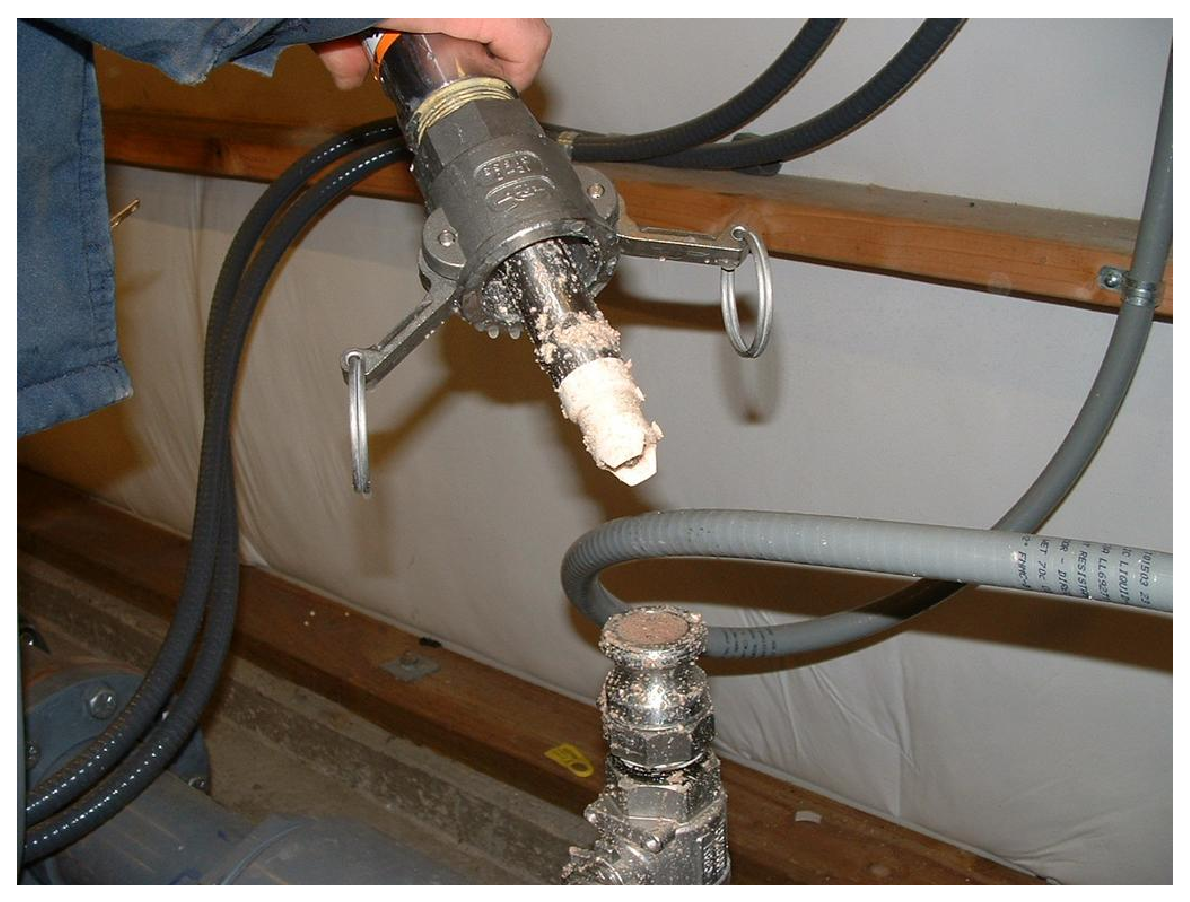
\includegraphics[width=5in]{ph_14.eps}$$

\filbreak

The voltage produced by the measurement electrode (glass membrane) is quite modest.  A calculation for voltage produced by a measurement electrode immersed in a 6.0 pH solution shows this.  First, we must calculate hydrogen ion concentration (activity) for a 6.0 pH solution, based on the definition of pH being the negative logarithm of hydrogen ion molarity:

$$\hbox{pH} = - \log[\hbox{H}^{+}]$$

$$6.0 = - \log[\hbox{H}^{+}]$$

$$-6.0 = \log[\hbox{H}^{+}]$$

$$10^{-6.0} = 10^{\log[\hbox{H}^{+}]}$$

$$10^{-6.0} = [\hbox{H}^{+}]$$

$$[\hbox{H}^{+}] = 1 \times 10^{-6} \> M$$

This tells us the concentration of hydrogen ions in the 6.0 pH solution\footnote{Hydrogen ion \textit{concentration} being practically the same as hydrogen ion \textit{activity} for dilute solutions.  In highly concentrated solutions, hydrogen ion concentration may exceed hydrogen ion activity because the ions may begin to interact with each other and with other ion species rather than act as independent entities.  The ratio of activity to concentration is called the \textit{activity coefficient} of the ion in that solution.}.  We know that the buffer solution inside the glass measurement bulb has a stable value of 7.0 pH (hydrogen ion concentration of $1 \times 10^{-7} \> M$, or 0.0000001 moles per liter), so all we need to do now is insert these values into the Nernst equation to see how much voltage the glass electrode should generate.  Assuming a solution temperature of 25 $^{o}$C (298.15 K), and knowing that $n$ in the Nernst equation will be equal to 1 (since each hydrogen ion has a single-value electrical charge):  \index{Nernst equation}

$$V = {{2.303 R T} \over {nF}} \log \left({C_1 \over C_2}\right)$$

$$V = {{(2.303)(8.315)(298.15)} \over {(1)(96485)}} \log \left({1 \times 10^{-6} \> M \over 1 \times 10^{-7} \> M}\right)$$

$$V = (59.17 \hbox{ mV}) (\log 10) = 59.17 \hbox{ mV}$$

We get the same result using our modified version of the Nernst equation:

$$V = {{2.303 R T} \over {nF}} \left(7 - \hbox{pH}_1 \right)$$

$$V = {{(2.303)(8.315)(298.15)} \over {(1)(96485)}} ( 7 - 6 )$$

$$V = (59.17 \hbox{ mV}) (1) = 59.17 \hbox{ mV}$$

If the measured solution had a value of 7.0 pH instead of 6.0 pH, there would be no voltage generated across the glass membrane since the two solutions' hydrogen ion activities would be equal.  Having a solution with one decade (ten times more: exactly one ``order of magnitude'') greater hydrogen ions activity than the internal buffer solution produces 59.17 millivolts at 25 degrees Celsius.  If the pH were to drop to 5.0 (two units away from 7.0 instead of one unit), the output voltage would be double: 118.3 millivolts.  If the solution's pH value were more alkaline than the internal buffer (for example, 8.0 pH), the voltage generated at the glass bulb would be the opposite polarity (e.g. 8.0 pH = $-59.17$ mV ; 9.0 pH = $-118.3$ mV, etc.).  

\filbreak

The following table shows the relationship between hydrogen ion activity, pH value, and probe voltage\footnote{The mathematical sign of probe voltage is arbitrary.  It depends entirely on whether we consider the reference (buffer) solution's hydrogen ion activity to be $C_1$ or $C_2$ in the equation.  Which ever way we choose to calculate this voltage, though, the polarity will be opposite for acidic pH values as compared to alkaline pH values}:

% No blank lines allowed between lines of an \halign structure!
% I use comments (%) instead, so Tex doesn't choke.

$$\vbox{\offinterlineskip
\halign{\strut
\vrule \quad\hfil # \ \hfil & 
\vrule \quad\hfil # \ \hfil & 
\vrule \quad\hfil # \ \hfil \vrule \cr
\noalign{\hrule}
%
% First row
\textbf{Hydrogen ion activity} & \textbf{pH value} & \textbf{Probe voltage} (at 25 $^{o}$C) \cr
%
\noalign{\hrule}
%
% Another row
$1 \times 10^{-3} \> M$ = 0.001 $M$ & 3.0 pH & 236.7 mV \cr
%
\noalign{\hrule}
%
% Another row
$1 \times 10^{-4} \> M$ = 0.0001 $M$ & 4.0 pH & 177.5 mV \cr
%
\noalign{\hrule}
%
% Another row
$1 \times 10^{-5} \> M$ = 0.00001 $M$ & 5.0 pH & 118.3 mV \cr
%
\noalign{\hrule}
%
% Another row
$1 \times 10^{-6} \> M$ = 0.000001 $M$ & 6.0 pH & 59.17 mV \cr
%
\noalign{\hrule}
%
% Another row
$1 \times 10^{-7} \> M$ = 0.0000001 $M$ & 7.0 pH & 0 mV \cr
%
\noalign{\hrule}
%
% Another row
$1 \times 10^{-8} \> M$ = 0.00000001 $M$ & 8.0 pH & $-59.17$ mV \cr
%
\noalign{\hrule}
%
% Another row
$1 \times 10^{-9} \> M$ = 0.000000001 $M$ & 9.0 pH & $-118.3$ mV \cr
%
\noalign{\hrule}
%
% Another row
$1 \times 10^{-10} \> M$ = 0.0000000001 $M$ & 10.0 pH & $-177.5$ mV \cr
%
\noalign{\hrule}
%
% Another row
$1 \times 10^{-11} \> M$ = 0.00000000001 $M$ & 11.0 pH & $-236.7$ mV \cr
%
\noalign{\hrule}
} % End of \halign 
}$$ % End of \vbox

This numerical progression is reminiscent of the \textit{Richter scale} used to measure earthquake magnitudes, where each ten-fold (decade) multiplication of power is represented by one more increment on the scale (e.g. a 6.0 Richter earthquake is ten times more powerful than a 5.0 Richter earthquake).  The logarithmic nature of the Nernst equation means that pH probes -- and in fact all potentiometric sensors based on the same dynamic of voltage produced by ion exchange across a membrane -- have astounding rangeability: they are capable of representing a wide range of conditions with a modest signal voltage span.  \index{Richter scale} \index{Rangeability}

Of course, the disadvantage of high rangeability is the potential for large pH measurement errors if the voltage detection within the pH instrument is even just a little bit inaccurate.  The problem is made even worse by the fact that the voltage measurement circuit has an extremely high impedance due to the presence of the \textit{glass} membrane\footnote{Glass is a very good insulator of electricity.  With a thin layer of glass being an essential part of the sensor circuit, the typical impedance of that circuit will lie in the range of \textit{hundreds} of mega-ohms!}.  The pH instrument measuring the voltage produced by a pH probe assembly must have an input impedance that is orders of magnitude greater yet, or else the probe's voltage signal will become ``loaded down'' by the voltmeter and not register accurately.  

\filbreak

Fortunately, modern operational amplifier circuits with field-effect transistor input stages are sufficient for this task\footnote{Operational amplifier circuits with field-effect transistor inputs may easily achieve input impedances in the \textit{tera-ohm} range ($1 \times 10^{12} \> \Omega$).}:

$$\includegraphics{ph_06.eps}$$

Even if we use a high-input-impedance pH instrument to sense the voltage output by the pH probe assembly, we may still encounter a problem created by the impedance of the glass electrode: an RC time constant created by the parasitic capacitance of the probe cable connecting the electrodes to the sensing instrument.  The glass electrode's enormous resistance value, combined with even a small amount of natural capacitance along the length of the cable, translates into a significant time delay imposed on the pH voltage signal.  The longer this cable is, the worse this time delay becomes due to increased capacitance:

$$\includegraphics{ph_07.eps}$$

\filbreak

This time constant value may be significant if the cable is long and/or the probe resistance is abnormally large.  Assuming a combined (measurement and reference) electrode resistance of 700 M$\Omega$ and a 30 foot length of RG-58U coaxial cable (at 28.5 pF capacitance per foot), the time constant will be:

$$\tau = RC$$

$$\tau = (700 \times 10^6 \> \Omega) \left( (28.5 \times 10^{-12} \hbox{ F/ft}) (30 \hbox{ ft}) \right)$$

$$\tau = (700 \times 10^6 \> \Omega)  (8.55 \times 10^{-10} \hbox{ F})$$

$$\tau = 0.599 \hbox{ seconds}$$

Considering the simple approximation of 5 time constants being the time necessary for a first-order system such as this to achieve within 1\% of its final value after a step-change, this means a sudden change in voltage at the pH probe caused by a sudden change in pH will not be fully registered by the pH instrument until almost 3 seconds after the event has passed!

It may seem impossible for a cable with capacitance measured in \textit{pico}farads to generate a time constant easily within the range of human perception, but it is indeed reasonable when you consider the exceptionally large resistance value of a glass pH measurement electrode.  For this reason, and also for the purpose of limiting the reception of external electrical ``noise,'' it is best to keep the cable length between pH probe and instrument as short as possible.

When short cable lengths are simply not practical, a \textit{preamplifier} module may be connected between the pH probe assembly and the pH instrument.  Such a device is essentially a unity-gain (gain = 1) amplifier designed to ``repeat'' the weak voltage output of the pH probe assembly in a much stronger (i.e. lower output impedance) form so the effects of cable capacitance will not be as severe.  A unity-gain operational amplifier ``voltage buffer'' circuit illustrates the concept of a preamplifier, with a typical output impedance in the hundreds (rather than \textit{millions}) of ohms: \index{Preamplifier, pH probe}

$$\includegraphics{ph_08.eps}$$

\filbreak

A preamplifier module appears in this next photograph:

$$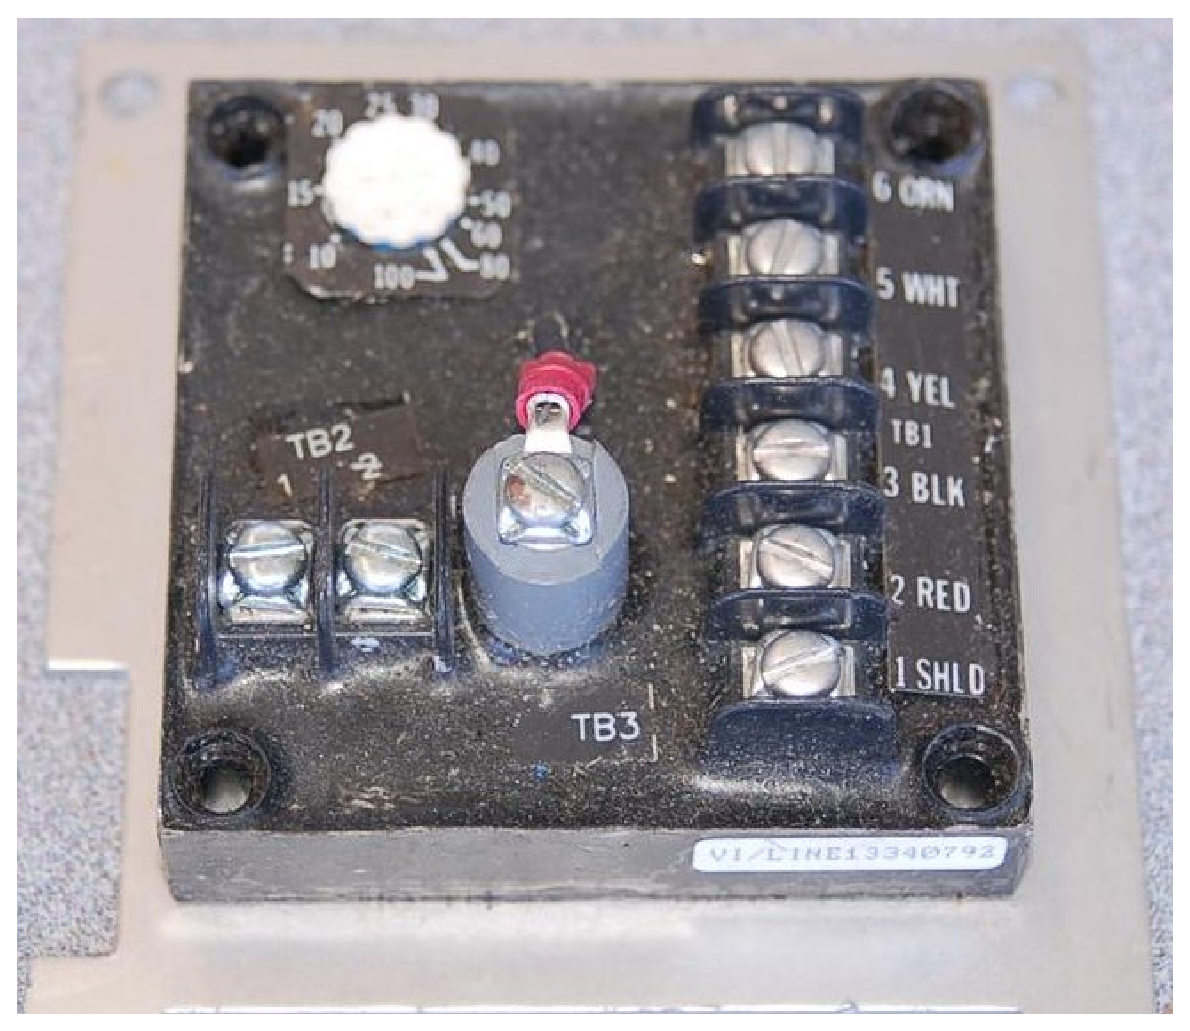
\includegraphics[width=3in]{ph_10.eps}$$

The preamplifier does not boost the probes' voltage output at all, nor does it eliminate the cable's capacitance.  Rather, the preamplified serves to decrease the impedance (the Th\'evenin equivalent resistance) of the probes by providing a low-resistance (relatively high-current capacity) voltage output to drive the cable and pH instrument.  By providing a voltage gain of 1, and a very large current gain, the preamplifier practically eliminates RC time constant problems caused by cable capacitance, and also helps reduce the effect of induced electrical noise.  As a consequence, the practical cable length limit is extended by orders of magnitude.

\filbreak

Some pH probe assemblies have built-in preamplifier circuits to boost the current-sourcing ability of the probe, rather than relying on a separate preamplifier module connected between the probe and pH instrument.  Preamplified pH probes have multi-conductor cables with extra wires used to conduct DC power from the pH transmitter to the pH probe to power the preamplifier:

$$\includegraphics{ph_18.eps}$$

\vskip 10pt

A feature seen in the above amplified probe is an \textit{RTD} sensor for detecting the temperature of the liquid process solution.  This is important because the Nernst equation contains a term for membrane temperature, which means the Nernst potential depends just as much on temperature as it does on ionic concentration.  The calculations we performed earlier predicting the amount of voltage produced by different solution pH values all assumed the same temperature: 25 degrees Celsius (298.15 Kelvin).  If the solution is not at room temperature, however, the voltage output by the pH probe will not be 59.17 millivolts per pH unit.  For example, if a glass measurement electrode is immersed in a solution having a pH value of 6.0 pH at 70 degrees Celsius (343.15 Kelvin), the voltage generated by that glass membrane will be 68.11 mV rather than 59.17 mV as it would be at 25 degrees Celsius.  That is to say, the \textit{slope} of the pH-to-voltage function will be 68.11 millivolts per pH unit rather than 59.17 millivolts per pH unit as it was at room temperature. \index{Slope, pH instrument}

The portion of the Nernst equation to the left of the logarithm function defines this slope value:

$$\hbox{Nernst potential} = {{2.303 R T} \over {nF}} \log \left({C_1 \over C_2}\right) = {{2.303 R T} \over {nF}} \left(7 - \hbox{pH}_1 \right)$$

$$\hbox{Slope} = {{2.303 R T} \over {nF}}$$

Recall that $R$ and $F$ are fundamental constants, and $n$ is fixed at a value of 1 for pH measurement (since there is exactly one electron exchanged for every H$^{+}$ ion migrating through the membrane).  This leaves temperature ($T$) as the only variable capable of influencing the theoretical slope of the function.

In order for a pH instrument to accurately infer a solution's pH value from the voltage generated by a glass electrode, it must ``know'' the expected slope of the Nernst equation.  Since the only variable in the Nernst equation besides the two ion concentration values ($C_1$ and $C_2$) is temperature ($T$), a simple temperature measurement will provide the pH instrument the information it needs to function accurately.  For this reason, many pH instruments are equipped with RTD inputs for solution temperature sensing, and many pH probe assemblies have built-in RTD temperature sensors ready to sense solution temperature.

\vskip 10pt

While the theoretical slope for a pH instrument depends on no variable but temperature, the \textit{actual} slope also depends on the condition of the measurement electrode.  For this reason, pH instruments need to be calibrated for the probes they connect to.  

A pH instrument is generally calibrated by performing a two-point test using \textit{buffer solutions} as the pH calibration standard.  A buffer solution is a specially formulated solution that maintains a stable pH value even under conditions of slight contamination.  For more information on pH buffer solutions, see section \ref{pH buffer} beginning on page \pageref{pH buffer}.  The pH probe assembly is inserted into a cup containing a buffer solution of known pH value, then the pH instrument is calibrated to that pH value\footnote{With all modern pH instruments being digital in design, this calibration process usually entails pressing a pushbutton on the faceplate of the instrument to ``tell'' it when the probe has stabilized in the buffer solution.  Clean and healthy pH probes typically stabilize to the buffer solution's pH value within 30 seconds of immersion.}.  After establishing the first calibration point, the pH probe is removed from the buffer, rinsed, then placed into another cup containing a second buffer with a different pH value.  After another stabilization period, the pH instrument is calibrated to this second pH value.  \index{Buffer solution}  \index{Calibration, pH instrument}

\filbreak

Only two points are necessary to define a line, so these two buffer measurements are all that is required by a pH instrument to define the linear transfer function relating probe voltage to solution pH:

$$\includegraphics{ph_09.eps}$$

Most modern pH instruments will display the calculated slope value after calibration.  This value should (ideally) be 59.17 millivolts per pH unit at 25 degrees Celsius, but it will likely be a bit less than this.  The voltage-generating ability of a glass electrode decays with age, so a low slope value may indicate a probe in need of replacement.

Another informative feature of the voltage/pH transfer function graph is the location of the \textit{isopotential} point: that point on the graph corresponding to zero probe voltage.  In theory, this point should correspond to a pH value of 7.0 pH.  However, if there exist stray potentials in the pH measurement circuit -- for example, voltage differences caused by ion mobility problems in the porous junction of the reference electrode, or contamination of the buffer solution inside the glass electrode bulb -- this point will shift.  Sufficient contamination of the buffer solution inside the measurement electrode (enough to drive its pH value from 7.0) will also cause an isopotential point shift, since the Nernst equation predicts zero voltage when ion concentrations on both sides of the membrane are equal.  

A quick way to check the isopotential point of a pH probe assembly is to short the input terminals on the pH measuring instrument together (forcing $V_{input}$ to be equal to 0 millivolts) and note the pH indication on the instrument's display\footnote{A more obvious test would be to directly measure the pH probe assembly's voltage while immersed in 7.0 pH buffer solution.  However, most portable voltmeters lack sufficient input impedance to perform this measurement, and so it is easier to calibrate the pH instrument in 7.0 pH buffer and then check \textit{its} zero-voltage pH value to see where the isopotential point is at.}.  This test should be performed \textit{after} calibrating the instrument using accurate pH buffer solutions.  The instrument characterized by the previous graph, for example, will register approximately 7.5 pH with its input terminals shorted because that is the pH value at which its probe happens to output zero millivolts.  \index{Isopotential point, pH}

When calibrating a pH instrument, you should choose buffers that most closely ``bracket'' the expected range of pH measurement in the process.  The most common buffer pH values are 4, 7, and 10.  For example, if you expect to measure pH values in the process ranging between 7.5 and 9, for example, you should calibrate that pH instrument using 7 and 10 buffers.

\vskip 10pt

Potentiometric pH probes require regular care and servicing for long life and accurate measurement.  For some pH probes, regular service includes refilling a liquid electrolyte reservoir for the reference electrode.  Cleaning is a common requirement for pH electrodes in dirty process applications such as wastewater.  Both the glass sensing bulb and the reference electrode must have direct contact with the process liquid, with no coating, plugging or other barriers to interfere with ion transfer.  If a pH probe is dirty, cleaning should be done with no solid contact made to the glass electrode because the glass electrode is very fragile.  Never use a toothbrush, a towel, or any sort of abrasive tool to clean a glass electrode!  Liquid probe-cleaning solutions are manufactured to dissolve a number of different types of fouling commonly found on pH probes:

\begin{itemize}
\item \textbf{Fats, greases, and oils} -- use a non-ionic surfactant or methanol solution
\item \textbf{Proteins} -- use an acidic pepsin solution
\item \textbf{Minerals} -- use an acidic solution
\item \textbf{Sulfides} -- use thiourea solution
\item \textbf{Microbial growth} -- use thiourea solution
\item \textbf{Salts} -- use deionized (distilled) water
\end{itemize}

Pressure-rinsing is a practical technique for cleaning stubborn deposits from pH probes.  A hand-pump squirt nozzle using cleaning solution (or in some cases, simply deionized water) is often able to dislodge the matter from a fouled pH probe.  Soaking in warm cleaning solution or deionized water is also recommended, especially for dislodging material from the small reference hole (allowing process fluid to reach the reference junction) found in many combination pH probes.  Regardless of the cleaning solution used, a thorough rinsing with deionized water is recommended as a final step before returning the pH probe to service.








% \filbreak
% \section{ORP measurement}

% ADD: text, illustrations, photos, etc.











\filbreak
\section{Chromatography}

Imagine a major marathon race, where hundreds of runners gather in one place to compete.  When the starting gun is fired, all the runners begin running the race, starting from the same location (the starting line) at the same time.  As the race progresses, the faster runners distance themselves from the slower runners, resulting in a dispersion of runners along the race course over time.

Now imagine a marathon race where certain runners share the exact same running speeds.  Suppose a group of runners in this marathon all run at exactly 8 miles per hour (MPH), while another group of runners in the race run a bit slower at exactly 6 miles per hour, and another group of runners plod along at exactly 5 miles per hour.  What would happen to these three groups of runners over time, supposing they all begin the race at the same location and at the exact same time?

As you can probably imagine, the runners within each speed group will stay with each other throughout the race, with the three groups becoming further spread apart over time.  The first of these three groups to cross the finish line will be the 8 MPH runners, followed by the 6 MPH runners a bit later, and then followed by the 5 MPH runners after that.  To an observer at the very start of the race, it would be difficult to tell exactly how many 6 MPH runners there were in the crowd, but to an observer at the finish line with a stop watch, it would be very easy to tell how many 6 MPH runners competed in the race, by counting how many runners crossed the finish line as a distinct group at the exact time corresponding to a speed of 6 MPH.

Now imagine a mixture of chemicals in a fluid state traveling through a very small-diameter ``capillary'' tube filled with an inert, porous material such as sand.  Some of those fluid molecules will progress more easily down the length of the tube than others, with similar molecules sharing similar propagation speeds.  Thus, a small sample of that chemical mixture injected into such a capillary tube, and carried along the tube by a continuous flow of solvent (gas or liquid), will tend to separate into its constituent components (called \textit{species}) over time just like the crowd of marathon runners separate over time according to running speed.  Slower-moving molecules will experience greater \textit{retention time} inside the capillary tube, while faster-moving molecules experience less.  A detector placed at the outlet of the capillary tube, configured to detect any chemical different from the solvent, will indicate the different species exiting the tube at different times.  If the retention time of each chemical species is known from prior tests, this device may be used to identify the composition of the original chemical mix (and even how much of each species was present in the injected sample) based solely on the \textit{time delay} of each species exiting the column.  More importantly, this one device will be able to identify and quantify a great many chemical compounds present in the original sample, a feat unmatched by most analytical technologies.  \index{Retention time}  \index{Species, chemical}

\vskip 10pt

This is the essence of \textit{chromatography}: the technique of chemical separation by time-delayed travel down the length of a stationary medium (called a \textit{column}).  In chromatography, the chemical solution traveling down the column is called the \textit{mobile phase}, while the solid and/or liquid substance residing within the column is called the \textit{stationary phase}.  Chromatography was first applied to chemical analysis by a Russian botanist named Mikhail Tswett, who was interested in separating mixtures of plant pigments.  The colorful bands left behind in the stationary phase by the separated pigments gave rise to the name ``chromatography,'' which literally means ``color writing.''  \index{Chromatography}  \index{Column, chromatograph}  \index{Mobile phase}  \index{Stationary phase}

Modern chemists often apply chromatographic techniques in the laboratory to purify chemical samples, and/or to measure the concentrations of different chemical substances within mixtures.  Some of these techniques are manual (such as in the case of \textit{thin-layer chromatography}, where liquid solvents carry liquid chemical mixtures along a flat plate covered with an inert coating such as alumina, and the positions of the chemical drops after time distinguishes one chemical species from another).  Other techniques are automated, with machines called \textit{chromatographs} performing the timed analysis of chemical travel through tightly-packed tubular columns.  The main focus of this section will be automated chromatography, as is used for continuous process analysis.





\filbreak
\subsection{Manual chromatography methods}

One of the manual chromatography methods taught to beginning chemists is \textit{thin-layer chromatography}, also known as \textit{TLC}.  An illustrated sequence showing thin-layer chromatography appears here:  \index{Thin-layer chromatography}

$$\includegraphics{chroma_01.eps}$$

The simplest forms of chromatography reveal the chemical composition of the analyzed mixture as residue retained by the stationary phase.  In the case of thin-layer chromatography, the different liquid compounds of the mobile phase remain embedded in the stationary phase at distinct locations after sufficient ``developing'' time.  The same is true in \textit{paper-strip chromatography} where a simple strip of filter paper serves as the stationary phase through which the mobile phase (liquid sample and solvent) travels: the different species of the sample remain in the paper as residue, their relative positions along the paper's length indicating their extent of travel during the test period.  If the chemical species happen to have different colors, the result will be a stratified pattern of colors on the paper strip\footnote{This effect is particularly striking when paper-strip chromatography is used to analyze the composition of \textit{ink}.  It is really quite amazing to see how many different colors are contained in plain ``black'' ink!}.  

% ADD: paper chromatography 
% --> pictures of paper used to separate inks, dyes

%\vskip 10pt

% ADD: column chromatography

%\vskip 10pt

% ADD: manual-injection gas chromatography




\filbreak
\subsection{Automated chromatographs}

The most common type of chromatography used in continuous process analysis is the \textit{gas chromatograph} (abbreviated ``GC''), so named because the mobile phase is a gas (or a vapor\footnote{Gas chromatographs are commonly used for industrial analysis on liquid sample streams, by using a heater at the inlet of the chromatograph to vaporize the liquid sample prior to analysis.  In such applications the column and sample valve(s) must be maintained in a heated condition as well so that the sample does not condense back into liquid form during the analysis.} rather than a liquid.  In a GC, the sample to be analyzed is injected at the head of a very long and very narrow tube packed with solid and/or liquid material\footnote{Stationary phase material used in many hydrocarbon GC's looks much like oily sand.}.  This long and narrow tube (called the \textit{column}) is designed to impede the passage of the sample molecules.  A continuous flow of ``carrier gas'' washes the sample compounds down the length of the column, allowing them to separate over time according to how they interact with the stationary phase packed inside the column.  A simplified schematic of a process GC shows how it functions:

$$\includegraphics{chroma_02.eps}$$

The \textit{sample valve} periodically injects a very precise quantity of sample into the entrance of the column tube and then shuts off to allow the constant-flow \textit{carrier} gas to wash this sample through the length of the column tube.  Each chemical species within the sample travels through the column at different rates, exiting the column at different times.  All the \textit{detector} needs to do is be able to tell the difference between pure carrier gas and carrier gas mixed with anything else.  

An important detail to note here is that the detector need not be discriminatory in its response to different chemical compounds, with just one exception: it need only distinguish between \textit{carrier} and \textit{non-carrier} compounds.  The ability for an analyzer to measure singular compounds out of a mixture is the fundamental challenge of all analytical instrumentation, and here we see the genius of chromatography: the variable we use to discriminate between different chemical compounds within the sample is \textit{retention time} through the column, and nothing else.  Rather than rely on some clever sensor technology to selectively detect one chemical compound out of a mixture, we are able to use a non-specific\footnote{This is not to say that one \textit{cannot} use a selective sensor as a chromatograph detector.  It's just that selectivity between different process compounds is not a \textit{necessary requirement} for a chromatograph detector.} sensor and let \textit{time} be the discriminating variable.  \index{Retention time}

Appealing to the marathon analogy again, it's as if a platform weigh-scale is situated at the finish line, to weigh the runners as they finish the race.  The scale cannot discern the running speed of any runner by their measured weight -- indeed, all the scale indicates is that \textit{someone} is crossing the finish line -- but it can determine the running speed based on \textit{when} the runner steps on the scale.

\vskip 10pt

\filbreak

If we plot the response of a chromatograph's detector on a graph, we see a pattern of peaks, each one indicating the departure of a species ``group'' (i.e. a different chemical compound) exiting the column.  This graph is typically called a \textit{chromatogram}: \index{Chromatogram}

$$\includegraphics{chroma_03.eps}$$

Narrow peaks represent compact bunches of molecules all exiting the column at nearly the same time, analogous to a group of runners crossing the finish line running shoulder-to-shoulder, all stepping on and off the platform scale at the same time.  Wide peaks represent more diffuse groupings of similar (or identical) molecules, analogous to a group of equally-fast runners crossing the finish line as a diffuse group.  In this chromatogram, you can see that species 4 and 5 are not clearly differentiated over time.  Better separation of species may be achieved by altering the sample volume, carrier gas flow rate, carrier gas pressure, type of carrier gas, column packing material, and/or column temperature.  




\filbreak
\subsection{Species identification}

Recall that the purpose of any analytical instrument is to discriminately measure \textit{one} variable or component concentration amongst a mix of different chemical components.  The fundamental challenge of chemical analysis is how to reliably and accurately detect that one ``species'' of chemical while being unaffected by the presence of any other chemical species.  Most analyzers rely on a sensor that exploits some unique characteristic of the chemical of interest (e.g. its unique ability to pass through a special membrane, its ability to absorb a unique spectrum of light, its tendency to engage in a unique chemical reaction, etc.), but not chromatographs.  Chromatographs simply delay the flow rate of different chemical species through a long tube based on those species' mass and interactions with the stationary phase, using \textit{time} as the discriminating variable.  This allows chromatographs to be nearly universal in the range of chemical species they can measure, while using relatively simple and uncomplicated detectors.  The detector need only discriminate between carrier gas and anything that isn't carrier gas in order to serve its purpose in a gas chromatograph.  Identifying a suitable detector technology is relatively easy given that fact that the type of carrier gas used in a GC is something \textit{chosen}\footnote{It should be noted that the choice of carrier for any chromatography system, be it manual or automated, is not completely arbitrary.  There are some limitations to which carrier fluids may be used, depending on the expected composition of the sample (e.g. you would not want to use a carrier that reacted chemically with any species in the sample so as to alter the sample's composition!).  However, the range of choices afforded to the person designing the chromatograph system lends a unique flexibility to this type of chemical analysis.} by the designer of the GC.  In other words, chromatography gives one the freedom to choose a compound that's easy for a sensor to detect, rather than try to find a sensor able to detect the specific species one needs to measure in the process.  This is important given the fact that there are many more types of chemical compounds in the world than there are chemical sensor types!    \index{Species, chemical composition}

In general, chemical compounds having less molecular weight tend to exit the column earlier, while compounds having greater molecular weight exit the column later.  The precise sequence of species elution through a column depends greatly on the stationary phase material type, as well as the carrier fluid type.  Proper selection of stationary phase and carrier compounds is essential to efficient chromatograph operation, and is usually the domain of trained chemists.

To view a flip-book animation showing how a chromatograph separates a sample into its constituent species, turn to Appendix \ref{chromatograph_simple} beginning on page \pageref{chromatograph_simple}.

\vskip 10pt

Since species identification in a chromatograph is performed with time as the discriminating factor, a chromatograph's ability to accurately identify chemical compounds depends on its control computer ``knowing'' when to expect various compounds to exit the column.  Chromatographs are calibrated by injecting a sample containing known concentrations of the species of interest (as well as any potentially interfering species), then timing the beginnings and ends of each species peak as each substance exits the column.

% ADD: "gate" times overlaid on chromatogram.  See Yamatake HGC303 datasheet for examples!







\filbreak
\subsection{Chromatograph detectors}

Several different detector designs exist for process gas chromatographs.  The two most common are the \textit{flame ionization detector} (FID) and the \textit{thermal conductivity detector} (TCD).  Other detector types include the \textit{flame photometric detector} (FPD), \textit{photoionization detector} (PID), \textit{nitrogen-phosphorus detector} (NPD), and \textit{ electron capture detector} (ECD).  All chromatograph detectors exploit some physical difference between the solutes\footnote{A ``solute'' being one of the sample species dissolved within the carrier gas} and the carrier gas itself which acts as a gaseous solvent, so that the detector may be able to detect the passage of solute molecules among carrier molecules.  \index{Flame photometric detector, GC}  \index{Nitrogen-phosphorus detector, GC}  \index{Electron capture detector, GC}  \index{Photoionization detector, GC}

\vskip 10pt

Flame ionization detectors work on the principle of ions liberated in the combustion of the sample species.  Here, the assumption is that sample compounds will ionize inside of a flame, whereas the carrier gas will not.  A permanent flame (usually fueled by hydrogen gas which produces negligible ions in combustion) serves to ionize any gas molecules exiting the chromatograph column that are not carrier gas.  Common carrier gases used with FID sensors are helium and nitrogen, which also produce negligible ions in a flame.  Molecules of sample encountering the flame ionize, causing the flame to become more electrically conductive than it was with only hydrogen and carrier gas.  This conductivity causes the detector circuit to respond with a measurable electrical signal.  A simplified diagram of an FID is shown here:

$$\includegraphics{chroma_17.eps}$$

Hydrocarbon molecules happen to easily ionize during combustion, which makes the FID sensor well-suited for GC analysis in the petrochemical industries where hydrocarbon composition is the most common form of analytical measurement\footnote{In fact, FID sensors are sometimes referred to as \textit{carbon counters}, since their response is almost directly proportional to the number of carbon atoms passing through the flame.}.  It should be noted, however, that not all carbon-containing compounds significantly ionize in a flame.  Examples of non-ionizing organic compounds include carbon monoxide, carbon dioxide, and carbon sulfide.  Other gases of common industrial interest such as water, hydrogen sulfide, sulfur dioxide, and ammonia likewise fail to ionize in a flame and thus are undetectable using an FID. \index{Flame ionization detector, GC}  


\vskip 10pt

Thermal conductivity detectors work on the principle of heat transfer by convection (gas cooling).  Here, the assumption is that sample compounds will have different thermal properties than the carrier gas.  Recall the dependence of a thermal mass flowmeter's calibration on the specific heat\footnote{See section \ref{thermal mass flowmeter specific heat} beginning on page \pageref{thermal mass flowmeter specific heat}.  The greater the specific heat value of a gas, the more heat energy it can carry away from a hot object through convection, all other factors being equal.} value of the gas being measured.  This dependence upon specific heat meant that we needed to know the specific heat value of the gas whose flow we intend to measure, or else the flowmeter's calibration would be in jeopardy.  Here, in the context of chromatograph detectors, we exploit the impact specific heat value has on thermal convection, using this principle to detect compositional change for a constant-flow gas rate.  The temperature change of a heated RTD or thermistor caused by exposure to a gas mixture with changing specific heat value indicates when a new sample species exits the chromatograph column.  \index{Thermal conductivity detector, GC}

A simplified diagram of a TCD is shown here, with pure carrier gas cooling two of the self-heated thermal sensors and sample gas (mixed with carrier gas, coming off the end of the column) cooling the other two self-heated sensors.  Differences in thermal conductivity between gas exiting the column versus pure carrier gas will cause the bridge circuit to unbalance, generating a voltage signal at the output of the operational amplifier circuit:

$$\includegraphics{chroma_18.eps}$$

This type of chromatograph detector works best, of course, when the carrier gas has a significantly different specific heat value than any of the sample compounds.  For this reason, hydrogen or helium (both gases having very high specific heat values compared to other gases) are the preferred carrier gases for chromatographs using thermal conductivity detectors.

% ADD: TCD schematic








\filbreak
\subsection{Measuring species concentration}

While \textit{time} is the variable used by a chromatograph to discriminate between different species (types) of chemical compounds, the concentration (quantity) of each chemical compound in the sample is inferred from the magnitude of the detector's response as it senses each compound.  Specifically, the quantity of each species present in the sample may be determined by applying the calculus technique of \textit{integration} to each chromatogram peak, calculating the area underneath each curve.  The vertical axis represents detector signal strength, which is proportional to the rate at which detected molecules are flowing through the sensor at any given time.  This means the height of each peak represents mass flow rate of each species ($W$, in units of micrograms per minute, or some similar units) passing through the detector.  The horizontal axis represents time, so therefore the integral (sum of infinitesimal products) of the detector signal over the time interval for any specific peak (time $t_1$ to $t_2$) represents a mass quantity that has passed through the column.  In simplified terms, a mass flow rate (micrograms per minute) multiplied by a time interval (minutes) equals mass in micrograms:  

$$m = \int_{t_1}^{t_2} W \> dt$$

\noindent
Where,

$m$ = Mass of sample species in micrograms

$W$ = Instantaneous mass flow rate of sample species in micrograms per minute

$t$ = Time in minutes ($t_1$ and $t_2$ are the interval times between which total mass is calculated)

\vskip 10pt

As is the case with all examples of integration, the unit of measurement for the totalized result is the \textit{product} of the units within the integrand: flow rate ($W$) in units of micrograms per minute multiplied by increments of time ($dt$) in the unit of minutes, summed together over an interval ($\int_{t_1}^{t_2}$), result in a mass quantity ($m$) expressed in the unit of micrograms.  Integration is really nothing more than the sum of products, with dimensional analysis working as it does with any product of two physical quantities:

$$\left({[\mu \hbox{g}] \over [\hbox{min}]}\right)  [\hbox{min}] = [\mu \hbox{g}]$$

\filbreak

This mathematical relationship may be seen in graphical form by shading the area underneath the peak of a chromatogram:

$$\includegraphics{chroma_04.eps}$$

Returning to the marathon analogy again, imagine the platform scale at the finish line being the detector, the race course being the chromatograph column, and the runners being individual molecules (each type of molecule running at its own unique speed).  If we wish to quantify how many runners of a certain speed were in the race, we would need to integrate the scale's weight reading during the time period in which we expect that class of runners to arrive at the finish line.  If a group of runners cross side-by-side such that they all step on the scale and leave the scale simultaneously, the scale's indication will be a tall and narrow peak when plotted on a time-based graph.  If an identical-size group of runners arrives at the finish line at some other time, but cross in single-file form rather than side-by-side, the scale will register each runner's weight one at a time with the graphed response being a much shorter and much wider peak.  In either group, though, it's the same number of runners finishing.  Therefore both the height of the peak (i.e. scale weight) and the duration of the peak need to be taken into consideration when calculating how many runners were in a particular group.

\vskip 10pt

Precise quantitative measurement of species concentration, however, is a bit more complicated than simply integrating detector peaks over time.  A problem we must deal with in chromatography is how a detector will respond differently to different chemical compounds.  Recall that the singular qualification for a gas chromatograph detector is its ability to detect species different from than the carrier gas: so long as the detector is able to sense the passage of compounds \textit{other} than carrier gas molecules, it is usable as a chromatograph detector.  This non-specificity of the detector is what makes chromatography such a versatile method for chemical analysis.  However, the simple requirement of being able to detect things other than carrier gas does not mean a detector will detect \textit{all} non-carrier substances \textit{equally}.  In fact, the opposite is almost always true: each detector type responds differently to different chemical compounds, which means the accumulated area underneath a peak on a chromatogram is not a pure representation of species mass, but rather it is a product of species mass and detector sensitivity to that species.

A flame ionization detector (FID), for example, responds more strongly to a given mass flow rate of butane (C$_{4}$H$_{10}$) than it does for the same mass flow rate of methane (CH$_{4}$), due to the greater carbon-per-mass ratio of butane.  This means  the ``raw'' chromatogram will reveal a peak of greater area for butane than it will for the same mass concentration of methane, simply because the detector is naturally more sensitive to the former compound than to the latter compound.

Thermal conductivity detectors (TCD) are not immune to this problem either.  TCDs exhibit varying responses to species having different specific heat and thermal conductivity coefficients.  That is to say, a given mass flow rate of butane through a TCD will yield a different level of response than the same mass flow rate of methane, simply because these two compounds exhibit different thermal properties.

The inconsistent response of a chromatograph detector to different sampled species is not as troubling a problem as one might think, though.  Since chromatographs operate on the principle of separating each species from the other over time, the chromatograph's control computer is ``aware'' of which chemical species is passing through the detector at any given time.  This fact allows us to program the computer with a set of pre-determined ``response factors'' describing how sensitive the detector is known to be for each species, allowing the computer to scale its interpretation of the detector's signal during each time period when a known species exits the column.  Thus, the chromatograph is able to calculate true mass concentration values based on measured peak areas and pre-programmed response factors.  \index{Response factor, chromatograph detector}

For example, knowing that a flame ionization detector (FID) is more sensitive to butane than it is to methane means the response factor for butane must be programmed such that it ``scales down'' the calculated mass based on the detector's raw signal during the time butane is expected to pass through it.  In other words, the chromatograph's computer ``shifts gears'' for each species exiting the column, during those times each expected species exits the column.

These detector response factors are determined by passing a mixture of known species proportions (a ``calibration gas'' sample) through the chromatograph, while programming the chromatograph computer with the known concentrations of this calibration gas.  As the chromatograph separates and measures each compound, it records the detector response to each one, calculating response factors to accurately equate detector response to the known concentrations in the calibration gas (usually scaled in percent or parts-per-million).  From then on, it will apply these ``response factor'' values to the raw detector signal, converting the detector's signal levels into equivalent concentration units.  

Most industrial process chromatographs come equipped with self-calibration ability, whereby calibration gas bottles stand connected to solenoid valves so that calibration gas may be directed to the analyzer on a pre-programmed schedule, with the chromatograph's microprocessor controller managing these calibration cycles all on its own.  This allows for frequent re-calibration of the chromatograph, to maintain its measurement accuracy over time with limited technician labor or oversight.





\filbreak
\subsection{Industrial applications of chromatographs}

Since process chromatographs have the ability to independently analyze the quantities of multiple species within a chemical sample, these instruments are inherently \textit{multi-variable}.  A single analog output signal (e.g. 4-20 mA) would only be able to transmit information about the concentration of any one species (i.e. any one peak) in the chromatogram.  This is perfectly adequate if only one species concentration is of interest in the process\footnote{It is not uncommon to find chromatographs used in processes to measure the concentration of a single chemical species, even though the device is capable of measuring the concentrations of multiple species within that process stream.  In those cases, chromatography is (or was at the time of installation) the most practical analytical technique to use for quantitative detection of that substance.  Why else use an inherently multi-variable analyzer when you could have used a single-variable technology that was simpler?  By analogy, it is possible to use a Coriolis flowmeter to measure nothing but fluid density, even though such a device is fully capable of measuring fluid density \textit{and} mass flow rate \textit{and} temperature.}, but some form of multi-channel digital (or multiple analog outputs) transmission is necessary to make full use of a chromatograph's ability.  Legacy chromatographs have multiple 4-20 mA analog output channels (one for each compound), while most modern chromatographs provide the option of digital bus communication (e.g. Modbus, FOUNDATION Fieldbus, etc.) to transmit data on multiple species concentrations to indicators, recorders, and/or controllers.  \index{Multi-variable transmitter}

\vskip 10pt

All modern chromatographs are ``smart'' instruments, containing one or more digital computers executing the calculations necessary to derive precise measurements from chromatogram data.  The computational power of modern chromatographs may be used to further analyze the process sample, beyond simple determinations of concentration or quantity.  Examples of more abstract analyses include approximate octane value of gasoline (based on the relative concentrations of several species), or the heating value of natural gas (based on the relative concentrations of methane, ethane, propane, butane, carbon dioxide, helium, etc. in a sample of natural gas).  

A very common industrial application of chromatographs is the monitoring and control of \textit{separation} processes such as distillation (or ``fractionation'') columns.  The purpose of any separation process is to take a mixture or a solution and force some of its constituent compounds apart into different fluid streams.  The ability of a chromatograph to measure multiple species within a sample makes it ideally suited for the task of quantifying the purity of the separated species exiting the separation process.  For example, a chromatograph may be used to analyze the purity of alcohol output by the fractionation column in a distillery, quantifying alcohol concentration, water concentration, and even the concentrations of various aromatic and flavoring compounds within the distillate fluid.  That data may be then used to alter some of the controlled parameters of the fractionation process such as feed flow rate, pressure, temperature gradient, etc. to achieve the desired product composition.  \index{Distillation}  \index{Fractionation}

Another industrial application of chromatography is the monitoring and control of chemical \textit{reaction} processes.  Once again we have a single instrument able to measure the concentration of desired product exiting the reaction, as well as unprocessed reactant species and also undesired products in the same product stream.  This data may then be used to control parameters in the chemical reactor to optimize the reaction taking place there.

\vskip 10pt

It should be noted that although \textit{gas} chromatography (GC) is far more prevalent in online industrial process analysis than liquid chromatography (LC), this does not mean the GC technique is limited to the analysis of process fluids existing in the gas phase alone.  Gas chromatographs are often used to analyze the composition of liquid process samples, by first boiling that liquid sample within the analyzer so it may be analyzed in gaseous form.  This means many of the species within the GC must be operated at temperatures exceeding the boiling point of the lowest-boiling-point substance in the sample.  While this poses certain technical challenges, it is nevertheless common practice in many industries.

\filbreak

The following photograph shows a gas chromatograph (GC) used to determine the heating value\footnote{Additionally, the data collected by this GC is used to improve the flow-measurement accuracy of their AGA3 honed-run orifice meters.  By measuring the concentrations of different compounds in the natural gas, the GC tabulates an average density for the gas, which is then sent to the flow computer to achieve better flow-measuring accuracy than would be possible without this compensating measurement.} of natural gas at a natural gas pipeline compression facility.  The entire instrument, from floor level to the top of the black box enclosing the chromatograph's column, is about 6 feet in height:

$$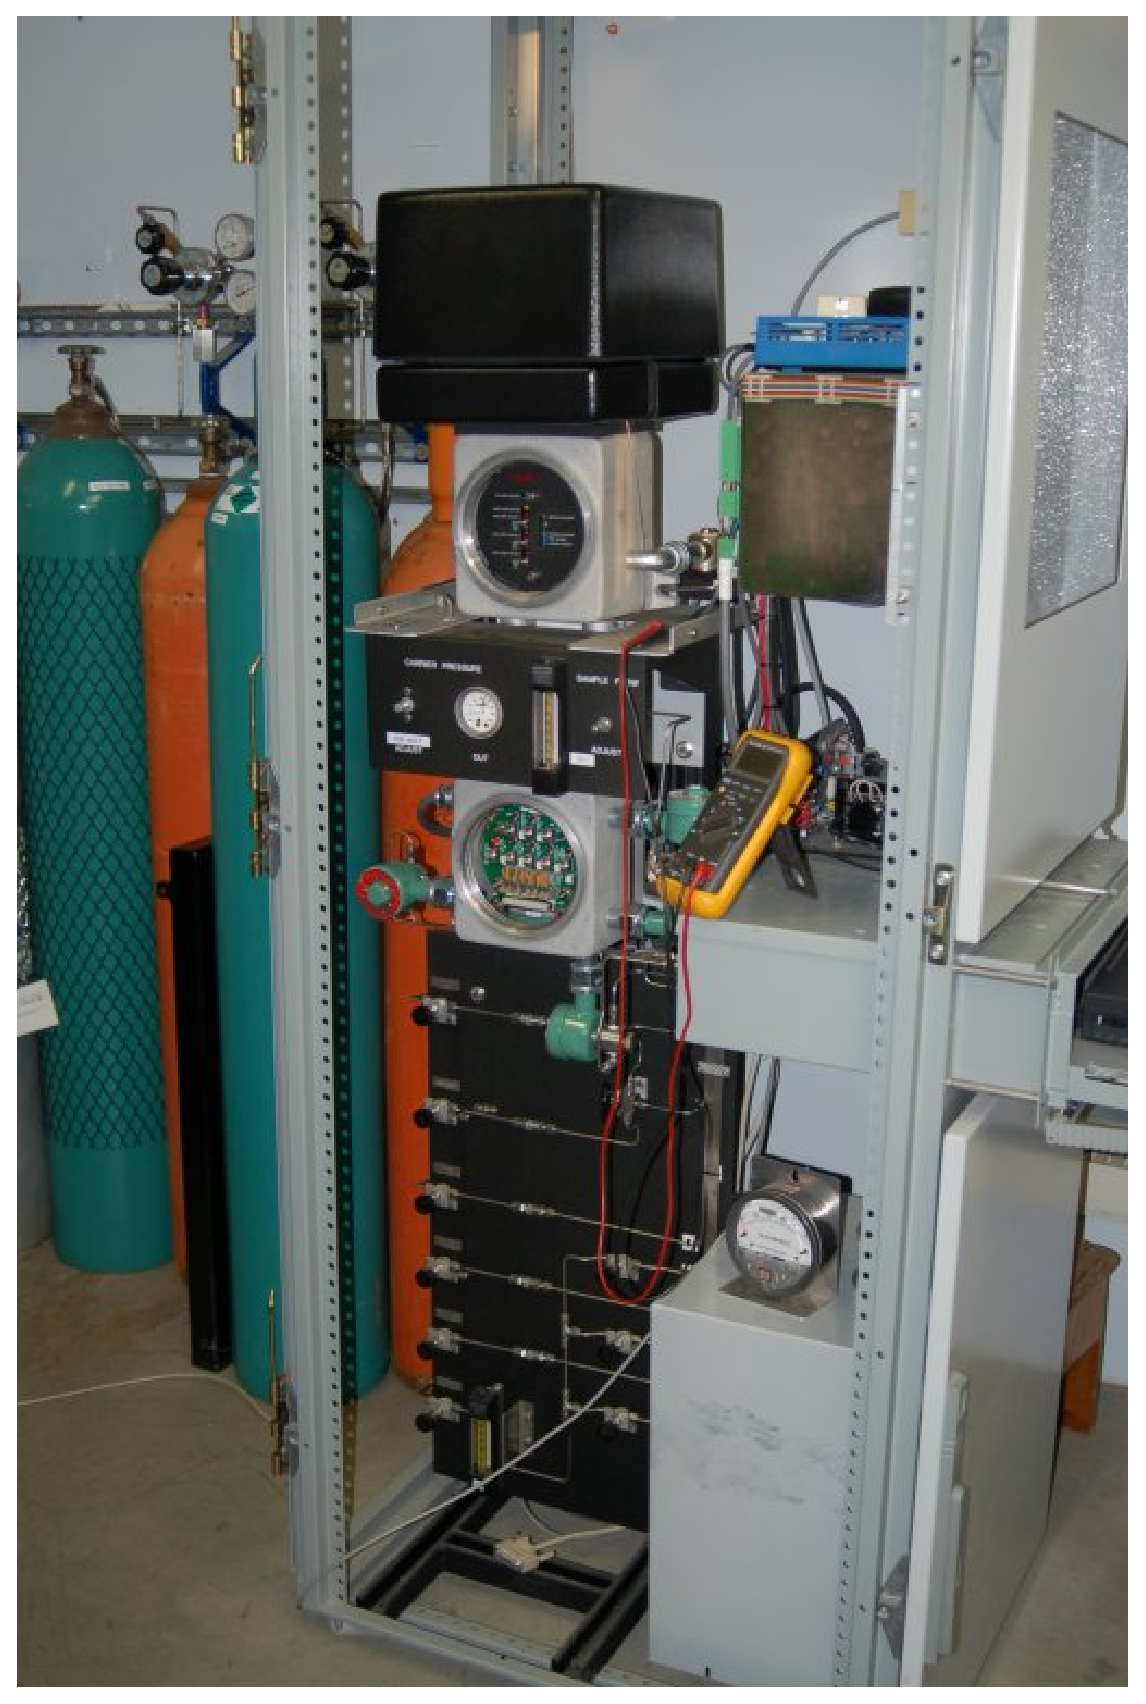
\includegraphics[height=3.5in]{chroma_05.eps}$$

This particular GC is used by a natural gas distribution company as part of its pricing system.  The heating value of the natural gas is used as data to calculate the selling price of the natural gas (dollars per standard cubic foot), so the customers pay only for the actual benefit of the gas (i.e. its ability to function as a fuel) and not just volumetric or mass quantity.  No chromatograph can directly measure the heating value of natural gas, but the analytical process of chromatography can determine the relative concentrations of compounds within the natural gas.  A computer, taking those concentration measurements and multiplying each one by the respective heating value of each compound, derives the gross heating value of the natural gas.

Although the column cannot be seen in this photograph of the GC, several high-pressure steel ``bottles'' may be seen in the background holding carrier gas used to wash the natural gas sample through the column.  

\filbreak

A typical gas chromatograph column appears in the next photograph.  It is nothing more than a stainless-steel tube packed with an inert, porous filling material:

$$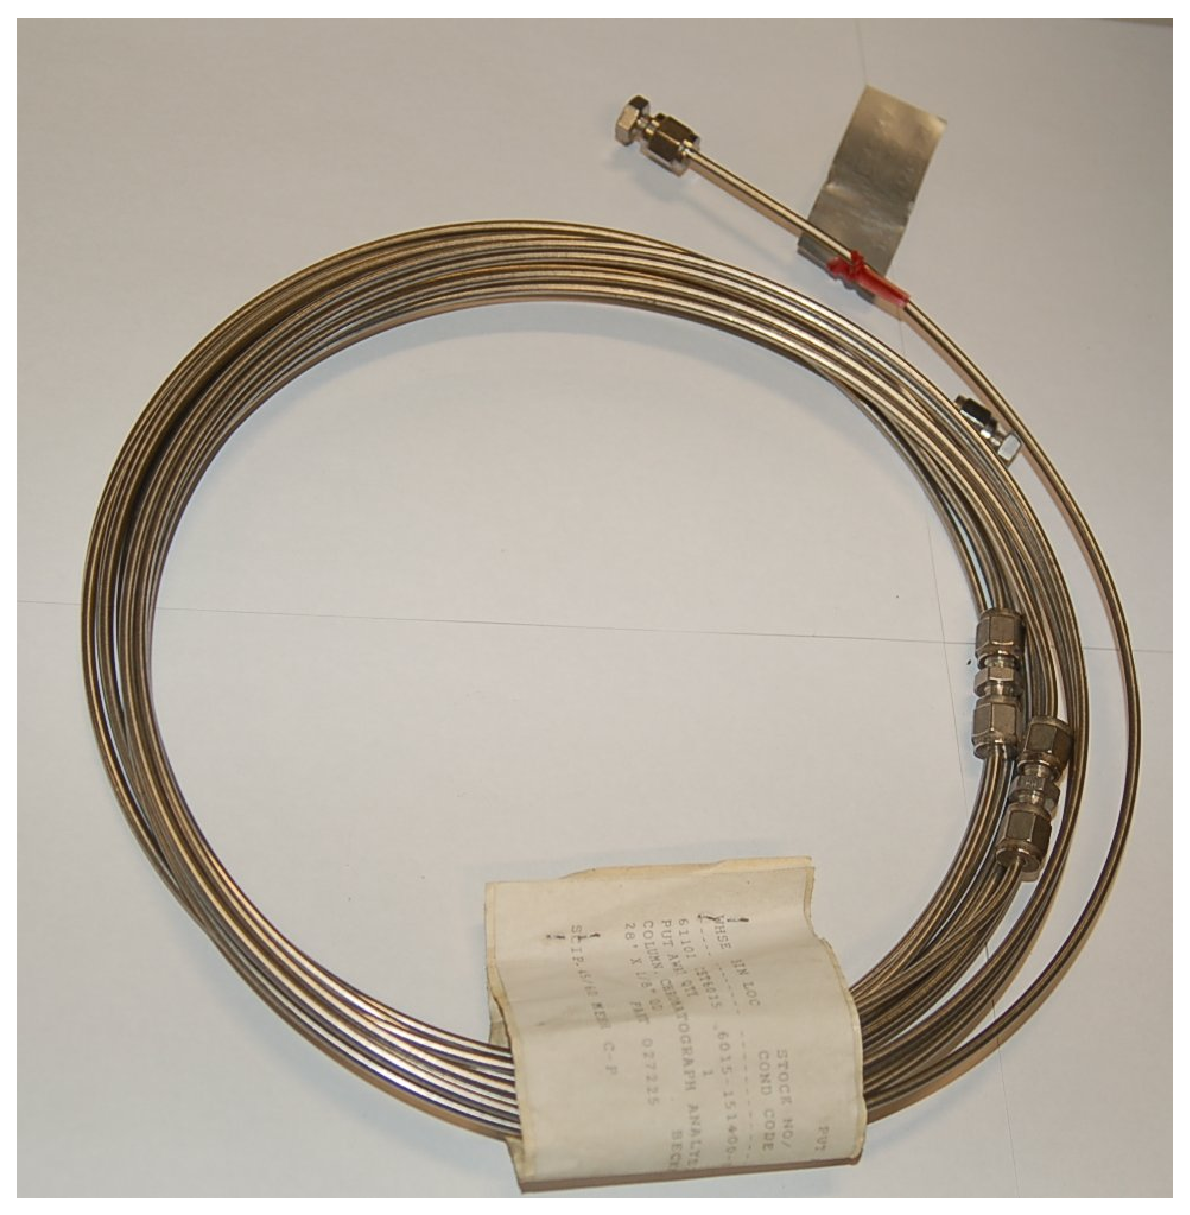
\includegraphics[width=5in]{chroma_06.eps}$$

This particular GC column is 28 feet long, with an \textit{outside} diameter of only 1/8 inch (the tube's inside diameter is even less than that).  Column geometry and packing material vary greatly with application.  The many choices intrinsic to column design are best left to specialists in the field of chromatography, not the average technician or even the average process engineer.

% ADD: use of chromatographs for distillation column composition control
% ADD: more photos of chromatographs, taken at Shell Puget Sound refinery with Mike Hoffman?







\filbreak
\subsection{Chromatograph sample valves}

Arguably, the component most critical to measurement accuracy in a gas chromatograph is the sample valve.  Its purpose is to inject the exact same sample quantity into the column at the beginning of each cycle.  If the sample quantity is not repeatable, the measured quantities exiting the column will change from cycle to cycle even if the sample composition does not change.  If the valve's cycle time is not repeatable, species separation efficiency will vary from cycle to cycle.  If the sample valve leaks such that a small flow rate of sample continuously enters the column, the result will be an altered ``baseline'' signal at the detector (at best) and total corruption of the analysis (at worst).  Many process chromatograph problems are caused by irregularities in the sample valve(s).

A photograph of the column (the coil of fine tubing about 6 inches in diameter, on the left) and sample valve (stainless-steel cylinder with several tubes entering and exiting, on the right) for a gas chromatograph appears here:

$$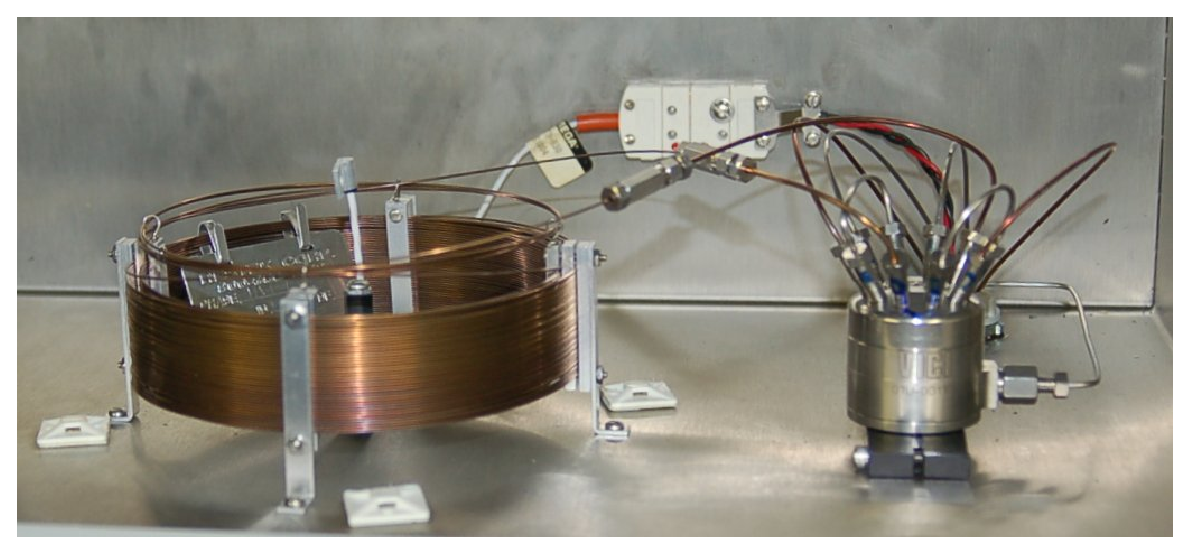
\includegraphics[width=4in]{chroma_16.eps}$$

\filbreak

A common form of sample valve uses a rotating element to switch port connections between the sample gas stream, carrier gas stream, and column:

$$\includegraphics{chroma_08.eps}$$

Three slots connect three pairs of ports together.  When the rotary valve actuates, the port connections switch, redirecting gas flows.

\filbreak

Connected to a sample stream, carrier stream, and column, the rotary sample valve operates in two different modes.  The first mode is a ``loading'' position where the sample stream flows through a short length of tubing (called a \textit{sample loop}) and exits to a waste discharge port, while the carrier gas flows through the column to wash the last sample through.  The second mode is a ``sampling'' position where the volume of sample gas held in the sample loop tubing gets injected into the column by a flow of carrier gas behind it:

$$\includegraphics{chroma_07.eps}$$

The purpose of the sample loop tube is to act as a holding reservoir for a fixed volume of sample gas.  When the sample valve switches to the sample position, the carrier gas will flush the contents of the sample loop toward the column.  This valve configuration guarantees that the injected sample volume cannot vary even if the sample valve's actuation is not precise.  The sample valve need only remain in the ``sampling'' position long enough to completely flush the sample loop tube, and the proper volume of injected sample gas is guaranteed.  An analogy for the sample loop is that of a measuring cup held underneath a continuously-spilling stream of water: so long as the cup is held beneath the stream long enough to completely fill, it is guaranteed to deliver a fixed volume of water when removed from the stream and emptied.  Over-filling the cup cannot result in an excessive sample size.  Like a measuring cup, the sample loop need only be filled completely with sample gas to deliver a fixed and unerring volume of gas to the chromatograph column when switched from the ``loading'' position to the ``sampling'' position.

While in the loading position, the stream of gas sampled from the process continuously fills the sample loop and then exits to a waste port.  This may seem wasteful but in fact is quite essential for practical sampling operation.  The volume of process gas injected into the chromatograph column during each cycle is so small (typically measured in units of \textit{micro}liters!) that a continuous flow of sample gas to waste is necessary to purge the impulse line connecting the analyzer to the process and thereby ensure a fresh sample, which in turn is necessary for the analyzer to obtain analyses of current conditions.  If it were not for the continuous flow of sample to waste, it would take a \textit{very long time} for a sample of process gas to make its way through the long impulse tube to the analyzer to be sampled, resulting in grossly delayed measurements of process conditions!

$$\includegraphics{chroma_09.eps}$$





\filbreak
\subsection{Improving chromatograph analysis time}

The ``Achilles heel'' of chromatography is the extraordinary length of time required to perform analyses, compared with many other analytical methods.  Cycle times measured in the range of minutes are not uncommon for chromatographs, even continuous ``on-line'' chromatographs used in industrial process control loops\footnote{Laboratory chromatographs may take even longer to complete their analyses.}!  It is the basic principle of chromatography to separate chemical species using time, and so a certain amount of measurement dead time is inevitable.  However, dead time in any measuring instrument is an undesirable quality.  Dead time in a feedback control loop is especially bad because enough of it will cause the loop to self-oscillate.  \index{Dead time}  \index{Transport delay}

One way to reduce the dead time of a chromatograph is to alter some of its operating parameters during the analysis cycle in such a way that it speeds up the progress of the mobile phase during periods of time where slowness of elution is not as important for fine separation of species.  The flow rate of the mobile phase may be altered, the temperature of the column may be ramped up or down, and even different columns may be switched into the mobile phase stream.  In chromatography, we refer to this on-line alteration of parameters as \textit{programming}.  \index{Programming, chromatograph}  \index{Flow programming, chromatograph} 

Temperature programming is an especially popular feature of process gas chromatographs, due to the direct effect temperature has on the viscosity of a flowing gas\footnote{Whereas most liquids decrease in viscosity as temperature rises, gases \textit{increase} in viscosity as they get hotter.  In other words, a gas becomes ``thicker'' as it heats up, thus slowing down its progress through a chromatograph column.  Since the flow regime through a chromatograph column is most definitely laminar and not turbulent, viscosity has a great effect on flow rate.}.  Carefully altering the operating temperature of a GC column while a sample washes through it is an excellent way to optimize the separation and time delay properties of a column, effectively realizing the high separation properties of a long column with the reduced dead time of a much shorter column:   \index{Temperature programming, chromatograph}

$$\includegraphics{chroma_10.eps}$$

\filbreak

Another way to speed up the analysis time of a chromatograph is to design it with multiple columns and multiple switching valves, timing the valves so that only the fastest species travel through all columns, while slower species bypass later column stages to exit through the detector first.  The alternative is to force all species to elute through all columns (or one long column), which means the minimum cycle time will be determined by the slowest species present in the sample.  To use the marathon analogy again, it's like having to wait until the very last runner crosses the finish line before we can start another race to challenge faster runners.  If, however, we stop the race mid-way to shuttle slow runners to the finish line (because we already know they are slow and will never win the race), we can still let the fastest runners compete the entire distance to determine who among them are the fastest, and thereby end the race sooner so we can move on to the next race:  \index{Dual-column chromatograph}  \index{Multi-column chromatograph}  \index{Chromatograph, dual-column}

$$\includegraphics{chroma_11.eps}$$

\filbreak

A sequence for one type of dual-column gas chromatograph begins with the sample valve injecting a precise quantity of sample into the first column.  In this illustration, the sample is comprised of 6 species labeled 1 through 6 in the order of their elution speed through the columns:

$$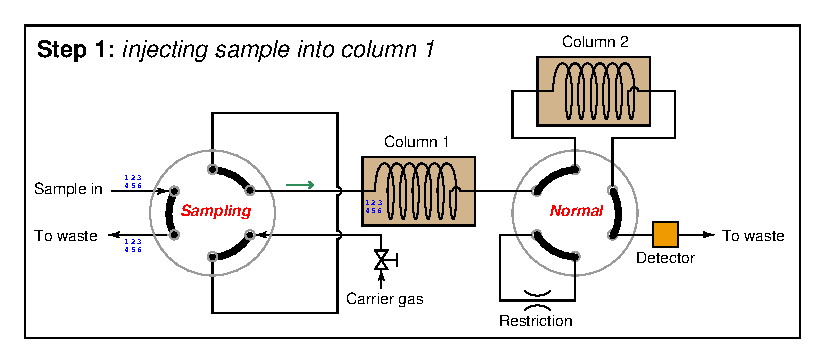
\includegraphics{chroma_12.eps}$$

In the next step, the six species elute through column 1, with species 1 through 3 making it into the second column while species 4 through 6 are still working their way through column 1:

$$\includegraphics{chroma_13.eps}$$

\filbreak

At this point in time, the dual-column valve switches into bypass mode, trapping the faster species (1 through 3) inside of column 2 while allowing the slower species (4 through 6) time to exit column 1 and pass through the detector:

$$\includegraphics{chroma_14.eps}$$

In the last step, the dual-column valve switches back to its normal mode, allowing species 1 through 3 to elute through column 2 and pass through the detector:

$$\includegraphics{chroma_15.eps}$$

The dual-column valve's timed switching from normal to bypass and back to normal again permits the slowest species to skip past the second column, while the fastest species must elute through \textit{both} columns for maximum separation.  This dual-column switching greatly reduces the total retention time of the sample without sacrificing separation of the fastest species\footnote{Since the degree of separation between species is roughly proportional to the species' retention time, the slowest species (4, 5, and 6 in this case) do not need to go through two columns to be adequately separated.  It is only the fastest species needing more retention time (through an additional column) to separate adequately from one another.}.  \index{Retention time}

\vskip 10pt

\filbreak

A few noteworthy points must be raised with regard to multi-column chromatographs.  First, the example shown in the preceding diagrams is not the only type of multi-column chromatograph.  ``Trapping'' a series of sample compounds inside a column is not the only way to provide different compounds with different column paths for faster separation.  Some multi-column chromatographs, for example, use ``backflush'' valves to reverse flow through one or more columns in an effort to avoid having the slowest species elute through the entire length of those columns.  This technique is used in applications where separation among compounds in the ``slow'' group is not important, since backflushing tends to reverse any separation that took place in the column previously.

The next point regarding multi-column chromatographs is that the dual-column valve timing must be precisely set according to known retention times of the different species inside the different columns.  In the example GC shown previously, this means the retention times of the transition species (3 and 4 in this case) through the first column must be precisely known, so the dual-column valve may be switched into bypass mode after species 3 exits the first column but before species 4 exits the first column.  The retention time of the slowest species (6) must also be precisely known so that the dual-column valve will not switch back to normal mode too soon and route any of that species into the second column where it would take much more time to leave the system.

A final point regarding multi-column chromatographs is that the order of species progression through the detector will \textit{not} be fastest to slowest as with single-column chromatographs.  In the dual-column GC shown previously, the slower group will exit first in order of speed (4, 5, 6), then the fastest group will exit last in order of speed (1, 2, 3).





\filbreak
\section{Introduction to optical analyses}

\label{Optical_analyzer_technology}

\textit{Light} is known to interact with matter in very specific ways, which may be exploited as a means of measuring chemical composition.  Either a sample of substance to be analyzed is stimulated into emitting light (optical \textit{emission}), or made to absorb light from an external source (optical \textit{absorption}).  The specific frequencies (colors) of light obtained from these analyses serve to identify the chemical elements and/or compounds present in the sample, and the relative intensities of each spectral pattern indicate the concentrations of those elements and/or compounds.

The theoretical basis for optical analysis is the interaction between charged particles of matter and light, which may be modeled both as a particle (called a \textit{photon}) and as an electromagnetic wave possessing a frequency ($f$) and a wavelength ($\lambda$).  Thanks to the work of the physicists Max Planck and Albert Einstein at the beginning of the 20th century, we know there is a definite proportionality between the frequency of a light wave and the amount of energy carried by each photon ($E$).  This proportionality is \textit{Planck's constant}, or $h$:  \index{Planck, Max}  \index{Einstein, Albert} \index{Planck's constant}

$$E = hf$$

\noindent
Where,

$E$ = Energy carried by a single ``photon'' of light (joules)

$h$ = Planck's constant (6.626 $\times$ $10^{-34}$ joule-seconds)

$f$ = Frequency of light wave (Hz, or 1/seconds)

\vskip 10pt

If the amount of energy carried by a photon happens to match the energy required to make an atomic electron ``jump'' from one energy level to another, the photon will be consumed in the work of that task when it strikes the atom.  Conversely, when that same electron returns to its original (lower) energy level in the atom, it releases a photon of the same frequency as the original photon that dislodged the electron.  Thus, energy is conserved (as always!): the energy received by the atom from the incident photon is later released in the form of another photon carrying the same amount of energy.

Since each element's electron configuration is unique, each element's electrons respond differently to light.  Both the colors (frequencies) of light required to boost electron energy levels and the colors (frequencies) of light emitted by those atoms as their electrons fall back to their original energy levels constitute a unique ``optical fingerprint'' for identifying elements.

\filbreak

Molecular motion (i.e. temperature) is also a source of photon emission.  Warm objects radiate energy in the form of electromagnetic radiation, which is why we are able to remotely measure the temperature of an object by the optical radiation it emits.

If we examine the visible light spectrum (a range of wavelengths spanning 700 nm to 400 nm, corresponding to a range of frequencies spanning $4.29 \times 10^{14}$ Hz to $7.5 \times 10^{14}$ Hz) emitted by a \textit{blackbody}\footnote{In physics, a ``blackbody'' is a perfect emitter of electromagnetic radiation (photons) as it is heated.  The intensity of light emitted as a function of wavelength ($\lambda$) and temperature ($T$) is $I = {{2 \pi h c^2 \lambda^{-5}} \over {e^{hc / \lambda k T} - 1}}$.} heated to a temperature of 5700 Kelvin, we see a continuous spectrum of color from violet on the left (short wavelength, high frequency, high energy) to red on the right (long wavelength, low frequency, low energy).  Here, I am using a computer program called \textit{Spectrum Explorer} (SPEX) to map both the color spectrum and the intensity of radiation across a range of wavelengths:

$$\includegraphics[width=5in]{optical_01.eps}$$

Unless the light from a heated blackbody passes through some device to separate it into its constituent colors, the human eye blends all the colors together and only sees \textit{white}.  Thus, we use the term ``white light'' to refer to an equal mixture of light frequencies covering the visible spectrum.  The grey areas to the far left and far right of the spectrum represent the ultraviolet and infrared regions, respectively, that lie outside of the human vision range.  A blackbody heated to 5700 K emits substantial quantities of both ultraviolet and infrared radiation, but this radiation is invisible to the human eye.

\filbreak

If we take a sample of pure hydrogen gas and heat it using an electric arc (inside a glass tube), the hydrogen atoms' electrons will be forced into higher energy states by the passage of electric current through the gas.  As those electrons fall back to lower original energy levels, they emit photons of characteristic wavelengths (color).  These wavelengths do \textit{not} cover the visible spectrum as they do for blackbody objects, but rather reveal themselves as thin ``lines'' on the visible spectrum range, and as ``peaks'' on the intensity plot:

$$\includegraphics[width=5in]{optical_03.eps}$$

Viewed with the unaided human eye, the light emitted from a hydrogen gas discharge tube looks bright red, because that is the predominant wavelength emitted.  The other colors tend to be overshadowed by the red, but we can still view them if we pass the light through a prism or through a diffraction grating to split it up into its constituent colors.

This particular set of ``lines'' is unique for the element hydrogen, and may serve as an identifying ``fingerprint'' for hydrogen if found in the emission spectrum for any chemical sample generated by the same method.

An alternative to electrically stimulating a quantity of hydrogen gas and thereby forcing an emission of specific wavelengths is to pass white light through a sample of hydrogen gas and then look for which colors are \textit{absorbed} by the gas.  As mentioned previously, photons having the necessary energies (frequencies) will become consumed in the work of elevating the hydrogen atoms' electrons to higher energy levels, leaving dark lines in an otherwise unbroken spectrum of colors from violet to red.  This is called the \textit{absorption spectrum} for an element, in contrast to the \textit{emission spectrum} obtained by electrically energizing atoms of that element to emit light.

\filbreak

The following illustration shows three different spectra: the \textit{full-color} (white light) spectrum of white light (top), the \textit{emission} spectrum of hydrogen gas (middle), and the \textit{absorption} spectrum of hydrogen gas (bottom).  Note how the dark gaps in the absorption spectrum precisely match the positions and colors of the bright lines in the emission spectrum, because the wavelengths of light \textit{absorbed} from white light as it passes through hydrogen gas are the exact same wavelengths \textit{emitted} by hydrogen gas when stimulated by an electric spark in a glass tube:

$$\includegraphics[width=6in]{optical_04.eps}$$

The dark lines found in the absorption spectrum constitute a distinctive ``fingerprint'' for the element hydrogen aligned with the colored lines in hydrogen's emission spectrum, and likewise may be used to detect the presence of hydrogen in gas samples through which white light is passed.  These dark spots in the spectrum are akin to ``shadows'' cast by molecules of hydrogen distributed throughout the sample gas.  A solid object casts a shadow whose outline represents the object's \textit{shape}.  A chemical compounds thoroughly dissolved in a solution, whether liquid or gas, casts a shadow whose attenuated wavelengths represent the compound's \textit{identity}. 

\vskip 10pt

Usually in industrial analysis we are more concerned with the quantifiable presence of certain \textit{compounds} in a process sample than we are in the presence of certain elements.  Fortunately, molecules also have their own distinctive\footnote{Molecules typically have much more complex interactions with light than individual atoms.  The optical signatures of atoms are principally defined by electron states, light absorbed when electrons are boosted into higher-energy states and light emitted when electrons fall into lower-energy states.  Molecules, on the other hand, can absorb and release energy in the inter-atomic bonds as well as in the states of individual electrons.  Since molecules have more degrees of freedom with respect to optical interactions, their optical signatures tend to be much broader.  This is why molecular absorption spectra consist of broad bands of wavelengths (each band comprised of many discrete lines), while atomic absorption spectra consist of relatively few lines.} interactions with light.  Sometimes, these interactions take the form of molecular electrons being boosted into higher energy levels, much the same as with individual atoms.  Other molecular-optical interactions take the form of \textit{vibrations} and \textit{rotations} set up between the atoms of a molecule, usually with photons in the infrared range\footnote{These photons have wavelengths longer than 700 nm, and so have energy values too low to boost electrons into higher levels.  However, the attractive bonds \textit{between} atoms in a molecule may be subject to the energy of these infrared photons, and so may dissipate the photons' energy and thereby attenuate a beam of infrared light.}.  As an infrared photon of the correct wavelength (energy value) strikes an appropriate molecule, its frequency resonates with the bonded atoms, almost as if they acted as miniscule masses connected together by coil springs.  This causes a transfer of energy from the photon to the molecule, where the vibration eventually dissipates that energy in the form of heat.

Thus, shining light through a sample of process gas, and analyzing the wavelengths absorbed by that gas sample, can provide quantitative measurements of the concentrations of certain gases types in that sample.

\filbreak

A few different infrared absorption spectra\footnote{In an absorption spectrum diagram, a non-absorbing substance results in a straight line at the 100\% mark.  Compounds absorbing specific wavelengths of light will produce low ``dips'' in the graph at those wavelength values, showing how less light (of those wavelengths) is able to pass un-absorbed through the sample to be detected at the other end.  By contrast \textit{emission} spectra are usually plotted with the characteristic wavelengths shown as high ``peaks'' in a graph that normally resides at 0\%.} for common industrial compounds are shown here, with the frequency shown in units of \textit{wavenumber} (the number of wavelengths per centimeter\footnote{Wavenumber, being the reciprocal of wavelengths in centimeters, may be thought of in terms of \textit{frequency}: the greater the wavenumber, the higher the frequency of the light wave (the smaller its wavelength).  In order to convert wavenumber into wavelength (in microns), reciprocate the wavenumber value and multiply by $10^4$.  For example, a wavenumber of 2000 cm$^{-1}$ is equivalent to a wavelength of 5 microns.  In order to convert wavenumber into wavelength (in nanometers), reciprocate the wavenumber value and multiply by $10^7$.  For example, a wavenumber of 4000 cm$^{-1}$ is equivalent to a wavelength of 2500 nm.}).  It should be noted that these absorption spectra are not drawn in scale to each other; rather, they are each drawn to their own scale to better show the relative sizes of the different absorption ``dips'' across the spectrum for each substance:  \index{Wavenumber}

$$\includegraphics{optical_13.eps}$$

Note that the pattern of each absorption spectrum is unique.  Each compound tends to absorb infrared light in its own way, and these ``signature'' absorption patterns provide us with a means to selectively identify the presence of various compounds in a process fluid sample.

Molecule types most effective at absorbing infrared light are those comprised of different atom types, such as carbon monoxide (CO), carbon dioxide (CO$_{2}$), sulfur dioxide (SO$_{2}$), water vapor (H$_{2}$O), and oxides of nitrogen (NO$_{x}$).  Molecules formed of two identical atoms such as molecular oxygen (O$_{2}$), nitrogen (N$_{2}$), and hydrogen (H$_{2}$) exhibit negligible interaction with infrared light.  This is a fortuitous quality of infrared analysis, because many process monitoring applications focus specifically on the former compounds to the exclusion of the latter.  Monitoring the exhaust emissions of a large combustion system, for example, is an application where the concentration(s) of CO, CO$_{2}$, SO$_{2}$, and/or NO$_{x}$ are relevant but the concentration of nitrogen (N$_{2}$) is not.  As with all chemical analyses, the key to selectivity is to find some property of measurement applicable only to the substance you are interested in measuring and not to any others.  This how analytical instruments discriminate between the substance of interest and the other ``background'' substances.  \index{Background substances}

\vskip 10pt

Between optical emission and optical absorption, absorption analysis seems to be the more popular in modern industrial use, with optical emission analysis limited mostly to laboratory applications.  One reason for this is the necessity of heating a sample to a high enough temperature for it to emit light: an energy-intensive and potentially hazardous endeavor.  Absorption analyzers need only shine a beam of light through an unheated sample chamber, then measure how much of specific wavelengths were absorbed by the sample.  Another important reason for the prevalence of absorption analyzers in industry is the necessity of a sophisticated computer and algorithm to sort the line spectra of substances generated in emission-type analyzers.  Inventors have devised clever ways to quantify the absorption spectra of different process substances without resorting to automated pattern-matching of spectra.

In every absorption-type optical analyzer, the fundamental equation relating photon absorption to substance concentration is the \textit{Beer-Lambert Law} (sometimes called the \textit{Lambert-Beer Law}):  \index{Beer-Lambert Law}  \index{Lambert-Beer Law}

$$A = abc = \log \left({I_0 \over I}\right)$$

\noindent
Where,

$A$ = Absorbance

$a$ = Extinction coefficient for photon-absorbing substance(s) 

$b$ = Path length of light traveling through the sample

$c$ = Concentration of photon-absorbing substance in the sample 

$I_0$ = Intensity of source (incident) light

$I$ = Intensity of received light after passing through the sample

\vskip 10pt

\filbreak

A typical arrangement for exposing a fluid sample (liquid or air) to light is shown in this diagram:

$$\includegraphics{optical_05.eps}$$

As indicated by the Beer-Lambert equation, greater sensitivity will be achieved with a longer path length.  In some applications where the substance of interest is an atmospheric pollutant, the light beam is simply shot through open air (usually reflecting on a mirror) before returning to the instrument for analysis.  If the light source happens to be a laser, the distance may be quite large\footnote{One such analyzer I saw in industry had a path length of a quarter-mile (1320 feet), to better measure extremely low concentrations of a gas!  The gas in question was ambient air inside of a large shelter housing a chemical process.  The analyzer was mounted on one side of the shelter, aiming a beam of laser light all the way to the opposite wall of the shelter 660 feet away, where a reflector was mounted.  The laser beam's path length was therefore twice the length of the shelter, or 1320 feet.}.

\vskip 10pt

Once the light has been passed through (or reflected off of) the process sample, it must be analyzed for attenuated wavelengths.  Two major types of wavelength analysis exist: \textit{dispersive} (where the light is split up into its constituent wavelengths) and \textit{nondispersive} (where the spectral distribution of the wavelengths is detected without separating colors).  These two optical analysis methods form the subject of the next two sections.








\filbreak
\section{Dispersive spectroscopy}

\index{Dispersive chemical analyzer}

The dispersion of visible light into its constituent colors goes all the way back to the 17th century with Isaac Newton's experiments, taking a glass \textit{prism} and generating the characteristic ``rainbow'' of colors:  \index{Prism}

$$\includegraphics{optical_06.eps}$$

A modern variation on the theme of a solid glass prism is a thin \textit{diffraction grating}, causing light of different wavelengths to ``bend'' as they pass through a series of very thin slits:  \index{Diffraction grating}

$$\includegraphics{optical_07.eps}$$

\filbreak

Some dispersive analyzers use a \textit{reflection grating} instead of a refraction grating.  Reflection gratings use fine lines etched on a reflective (mirror) surface to produce an equivalent dispersive effect to a diffraction grating\footnote{You may use an old compact disk (CD) as a simple reflection and refraction grating.  Holding the CD with the reflective (shiny) surface angled toward you, light reflected from a bright source such as a lamp (avoid using the sun, as you can easily damage your eyes viewing reflected sunlight!) will split into its constituent colors by reflection off the CD's surface.  Lines in the plastic of the CD perform the dispersion of wavelengths.  You will likely have to experiment with the angle you hold the CD, pointing it more perpendicular to the lamp's direction and more angled to your eyes, before you see the image of the lamp ``smeared'' as a colorful spectrum.  To use the CD as a diffraction grating, you will have to carefully peel the reflective aluminum foil off the front side of the disk.  Use a sharp tool to scribe the disk's front surface from center to outer edge (tracing a radius line), then use sticky tape to carefully peel the scribed foil off the plastic disk.  When you are finished removing all the foil, you may look \textit{through} the transparent plastic and see spectra from light sources on the other side.  Once again, experimentation is in order to find the optimum viewing angle, and be sure to avoid looking at the sun this way!}:  \index{Reflection grating}

$$\includegraphics{optical_09.eps}$$

In 1814, the German physicist Joseph von Fraunhofer closely analyzed the spectrum of colors obtained from sunlight and noticed the existence of several dark bands in the otherwise uninterrupted spectrum where specific colors seemed to be attenuated.  Later that century, experiments by the French physicist Jean Bernard L\'eon Foucault and the German physicist Gustav Robert Kirchoff confirmed the same effect when white light was passed through a vapor of sodium.  They correctly reasoned that the sun's core produced a continuous spectrum\footnote{One might wonder why the sun does not produce a line-type emission spectrum of all its constituent elements, instead of the continuous spectrum it does.  The answer to this question is that emission spectra are produced only when the ``excited'' atoms are in relative isolation from each other, such as is the case in a low-pressure gas.  In solids, liquids, and high-pressure gases, the close proximity of the atoms to each other creates many different opportunities for electrons to ``jump'' to lower energy levels.  With all those different alternatives, the electrons emit a whole range of different wavelength photons as they seek lower energy levels, not just the few wavelengths associated with the limited energy levels offered by an isolated atom.  We see the same effect on Earth when we heat metals: the electrons in a solid or liquid metal sample have so many different optional energy levels to ``fall'' to, they end up emitting a broad spectrum of wavelengths instead of just a few.  In this way, a molten metal is a good approximation of a blackbody photon source.} of light (all wavelengths) due to its incredibly high temperature, but that certain gaseous elements (including sodium) in the cooler, outer ``atmosphere'' of the sun were absorbing some of the wavelengths to cause the \textit{Fraunhofer lines} in the observed spectrum.  These scientists noted the same patterns of absorption (dark lines) in the sun's spectrum that appeared in laboratory absorption tests with sodium.  The implication of these scientists' experiments are truly staggering, as they were able to correctly identify gaseous elements in a sample \textit{93 million miles distant from Earth!}.  \index{Fraunhofer, Joseph von} \index{Fraunhofer lines}

This sort of spectrographic analysis is called \textit{dispersive}, because it relies on a device such as a prism or diffraction grating to \textit{disperse} the different wavelengths of light from each other so they may be independently measured.

\filbreak

A dispersive analyzer for process fluids would be constructed in this manner, introducing incident light to a windowed sample chamber where some wavelengths of that light would be attenuated by interaction with the process fluid molecules.  In this illustration, the sample gas absorbs some of the yellow light wavelengths, resulting in less yellow light reaching the detector array:

$$\includegraphics{optical_08.eps}$$

The light source need not output white light if the wavelengths of interest do not span the entire visible spectrum.  For example, if the absorption spectrum of a particular substance is known to primarily span infrared light and not the visible range, it may be sufficient to use a dispersive analyzer with an infrared light source rather than a ``broad spectrum'' light source covering both the infrared and visible ranges.

A necessary component of any dispersive analyzer is a computer connected to the detector array with the ability to recognize all expected emission spectra patterns, and quantify them based on the relative strengths of the detected wavelengths.  This is a level of sophistication beyond most industrial measuring instruments at the time of this writing (2015), which is one reason dispersive analyzers are not as popular (yet!) for industrial process use.  However, once such a computer and necessary software are in place to perform the analyses, measurement of multiple substances from the same absorption spectrum becomes possible.  Like chromatographs, dispersive optical analyzers naturally function as multi-component measurement devices.








\filbreak
\section{Non-dispersive Luft detector spectroscopy}

\label{Nondispersive_chemical_analyzer}
\index{Non-dispersive chemical analyzer}

Non-dispersive analysis, while newer in discovery than dispersive analysis (Isaac Newton's 17th-century prism), has actually seen far earlier application as continuous process analyzers.  The basic design was developed during the years 1937-1938 by Dr. Luft and Dr. Lehrer in the laboratories of the German chemical company \textit{I.G. Farbenindustrie}.  By the end of World War II, over four hundred of these innovative instruments were in service in German chemical plants.  Unlike most industrial analyzer technologies which are nothing more than adaptations of laboratory tests previously used by chemists to take manual measurements of substances, the invention of the first non-dispersive process gas analyzer embodied a wholly new analytical technique.  

% ADD: details from Dr. Luft's paper ``Zeitschrift fur Technische Physik'' volume 24, Number 5, (1943) pp. 97-104.

Industrial non-dispersive analyzers typically use either infrared or ultraviolet light sources, because most substances of interest absorb wavelengths in those regions rather than in the visible light spectrum.  Non-dispersive spectroscopy using infrared light is usually abbreviated \textit{NDIR}, while non-dispersive spectroscopy using ultraviolet light is abbreviated \textit{NDUV} and non-dispersive spectroscopy using visible light is abbreviated \textit{NDVIS}.  Historically, NDIR is the more prevalent of the three technologies.  Also, \textit{gas} analysis is the more common application of non-dispersive spectroscopy in industry, as opposed to \textit{liquid} analysis, which is why all the examples in this portion of the book assume the analysis of a process gas.  \index{NDIR spectroscopy}  \index{NDUV spectroscopy}  \index{NDVIS spectroscopy}

\filbreak

A partial listing of NDIR gas analysis applications at the I.G. Farben synthetic rubber facility in H\"uls, Germany at the conclusion of World War II is shown here\footnote{These details taken from pages 93-94 of \textit{Instrumentation and Control in the German Chemical Industry}, a fascinating book detailing the state-of-the-art in process instrumentation in German chemical manufacturing facilities following the war.}.  Note the impressive diversity of ranges and gases of interest measured by NDIR analyzers at this time in history, less than ten years following the invention of the technique:

% No blank lines allowed between lines of an \halign structure!
% I use comments (%) instead, so that TeX doesn't choke.

$$\vbox{\offinterlineskip
\halign{\strut
\vrule \quad\hfil # \ \hfil & 
\vrule \quad\hfil # \ \hfil & 
\vrule \quad\hfil # \ \hfil \vrule \cr
\noalign{\hrule}
%
% First row
\textbf{Gas of interest} & \textbf{Range} & \textbf{Other gases present in mixture} \cr
%
\noalign{\hrule}
%
% Another row
Carbon monoxide & 0 to 0.05\% & Hydrogen \cr
 & 0 to 0.1\% &  \cr
%
\noalign{\hrule}
%
% Another row
Carbon monoxide & 0 to 30\% & Nitrogen, methane, ethane \cr
%
\noalign{\hrule}
%
% Another row
Carbon dioxide & 0 to 0.1\% & Atmospheric air (nitrogen, oxygen, argon) \cr
%
\noalign{\hrule}
%
% Another row
Carbon dioxide & 0 to 0.5\% & Hydrogen, methane, ethylene \cr
%
\noalign{\hrule}
%
% Another row
Carbon dioxide & 0 to 2\% & Acetylene \cr
%
\noalign{\hrule}
%
% Another row
Carbon dioxide & 0 to 10\% & Acetylene, ethylene \cr
%
\noalign{\hrule}
%
% Another row
Acetylene & 0 to 2\% & Hydrogen, ethylene, methane, ethane \cr
%
\noalign{\hrule}
%
% Another row
Acetylene & 0 to 5\% & Ethylene \cr
%
\noalign{\hrule}
%
% Another row
Acetylene & 0 to 10\% & Ethylene, methane, ethane \cr
%
\noalign{\hrule}
%
% Another row
Acetylene & 0 to 40\% & Ethylene, propylene, methane, ethane \cr
%
\noalign{\hrule}
%
% Another row
Acetylene & 30 to 80\% & Hydrogen, ethylene, methane, ethane \cr
%
\noalign{\hrule}
%
% Another row
Acetylene & 50 to 100\% & Ethylene, propylene, methane, ethane \cr
 &  & Ethylene, ethane, methane \cr
 &  & Hydrogen, ethylene, methane, ethane \cr
%
\noalign{\hrule}
%
% Another row
Butadiene & 0 to 1\% & Atmospheric air (nitrogen, oxygen, argon) \cr
%
\noalign{\hrule}
%
% Another row
Ethylene & 0 to 10\% & Acetylene, methane, ethane, \cr
 &  & propylene, dinitrogen dioxide \cr
%
\noalign{\hrule}
%
% Another row
Ethylene & 0 to 30\% & Methane, ethane \cr
%
\noalign{\hrule}
%
% Another row
Ethylene & 0 to 40\% & Carbon dioxide, chlorine, \cr
 &  & propylene, acetylene \cr
%
\noalign{\hrule}
%
% Another row
Ethylene & 40 to 80\% & Ethylene, acetylene, dinitrogen dioxide \cr
%
\noalign{\hrule}
%
% Another row
Ethylene & 80 to 100\% & Methane, ethane \cr
%
\noalign{\hrule}
%
% Another row
Methane & 75 to 100\% & Ethylene, ethane \cr
%
\noalign{\hrule}
} % End of \halign 
}$$ % End of \vbox

At a different I.G. Farben facility (in Uerdingen, Germany), an NDIR instrument was used as a safety gas detector for carbon monoxide (0 to 0.1\% concentration) in open air.  This was in a process area where high concentrations of carbon monoxide gas existed in the lines, and where a leak in a process line or valve posed a considerable safety hazard to personnel.

\vskip 10pt

The challenge of any analytical measurement technology is how to achieve selectivity, where the analyzing instrument responds to the concentration of just one substance (one ``species'') and to \textit{no other substance(s) in the mixture}.  If the substance of interest exhibits some unique physical property we can readily measure with sensors, the selectivity problem is easy to solve: just measure that one property exclusively, and no other substance will interfere.  \index{Species, chemical composition}

In the case of absorption spectrometers such as non-dispersive analyzers, the challenge is to selectively measure the concentration of certain light-absorbing substances amidst the presence of other substances also absorbing certain wavelengths of light.  If the substance of interest is the \textit{only} substance present in the mixture capable of absorbing light, selectivity is guaranteed.  However, most applications in industry are not this easy, with the mixture containing other light-absorbing substances besides the one of interest.  Some of these substances may absorb completely different wavelengths of light, while others may have absorption bands overlapping the absorption bands of the substance of interest (i.e. the interfering substances absorb some of the same wavelengths of light absorbed by the substance of interest, in addition to absorbing some unique wavelengths of their own).

Dispersive spectrographs achieve selectivity by ``disassembling'' the spectrum into individual wavelengths and measuring them one by one, but a non-dispersive analyzer must somehow distinguish different spectral responses without this ``disassembly'' of wavelengths.  The bulk of this section is devoted to a discussion of exactly how selectivity is accomplished using the NDIR technique.







\filbreak
\subsection{Single-beam analyzer}

Non-dispersive analyzers employ the principle of spectrographic \textit{absorption} to measure how much of a particular substance exists within a sample.  NDIR gas analyzers shine light through a windowed sample chamber (typically called a \textit{cell}), through which a fresh flow of process gas continually moves.  Certain ``species'' (compounds) of gas within the sample stream absorb part of the incident light, and therefore the light exiting the cell becomes partially depleted of those wavelengths.  A heat-sensitive detector placed behind the cell measures how much infrared light did not get absorbed by the sample gas.  If we imagine the concentration of light-absorbing gas increasing over time, more of the infrared light entering the cell will being absorbed by the gas and converted into heat within the cell, leaving less light exiting the cell to generate heat at the detector.  The simplest style of non-dispersive analyzer uses a single light source, shining continuously through a single gas cell, and eventually falling on a small thermopile (converting the received infrared light into heat, and then into a voltage signal):  \index{Species, chemical composition}

$$\includegraphics{optical_12.eps}$$ % Single-beam with nonspecific detector

This crude analyzer suffers from multiple problems.  First, it is non-selective: \textit{any} light-absorbing gas entering the sample cell reduces heat at the detector (i.e. generates less thermopile voltage), regardless of the species.  It might work well enough in an application where the only light-absorbing gas in the process mixture happens to be the one gas we are interested in measuring, but most industrial analyzer applications are not like this.  In most cases, our process sample contains multiple species of gases capable of absorbing light within a similar range of wavelengths, but we are only interested in measuring one of them.  An example would be the measurement of carbon dioxide (CO$_{2}$) concentration in the exhaust gas of a combustion furnace: most of the gases exiting the furnace do not absorb infrared light (nitrogen, oxygen), but CO$_{2}$ gas does.  However, carbon monoxide (CO), water vapor (H$_{2}$O), and sulfur dioxide (SO$_{2}$) also absorb infrared light, and are all normally present in the exhaust gas of a furnace to varying degrees.  Since our crude NDIR analyzer is non-selective, it cannot differentiate between carbon dioxide and any of the other infrared-absorbing gases present in the exhaust gas.

Another significant problem with this analyzer design is that any variations in the light source's output cause both a zero shift and a span shift in the instrument's calibration.  Since light sources tend to weaken with age, this flaw necessitates frequent re-calibration of the analyzer.

Finally, since the detector is a thermopile, its output will be affected not just by the light falling on it, but also by ambient temperature, causing the analyzer's output to vary in ways completely unrelated to sample gas composition.





\filbreak
\subsection{Dual-beam analyzer}

One way to improve on the single-beam analyzer design is to split the light beam into two equal halves, then pass each half-beam through its own cell.  Only one of these cells will hold the process gas to be analyzed -- the other cell is sealed, containing a ``reference'' gas such as nitrogen that absorbs no infrared light.  At the end of each cell we will place a matched pair of thermopile detectors, connecting these detectors in series-opposing fashion so equal voltages will cancel:

$$\includegraphics{optical_14.eps}$$ % Dual-beam with nonspecific detector (no chopper)

Let us perform some ``thought experiments'' on this apparatus to explore its behavior.  Imagine the sample gas being a non-absorber of infrared light just like the reference gas.  In this virtual experiment, the opposed detector pair will generate no voltage signal because each of the two detectors receives the same (full) amount of incident light.   \index{Thought experiment}  \index{Problem-solving technique: thought experiment} 

Next, we will alter one of the variables in our ``thought experiment'' to see what difference that variable makes.  Here, we imagine the sample containing some concentration of an infrared-absorbing gas while the reference gas continues to absorb no light.  Now, the two thermopile detectors will receive differing intensities of infrared light, causing the series-opposed pair to be out of balance, generating a net voltage signal we can measure as an indication of light-absorbing gas concentration.

The addition of a reference gas chamber and second thermopile detector completely eliminates the ambient temperature problem seen in the single-detector apparatus.  If the analyzer's temperature happens to rise or fall, the voltages output by \textit{both} thermopiles will rise and fall equally, canceling each other out so that the only voltage produced by the series-opposing pair will be that produced by differences in received light intensity.

The dual-detector design also eliminates the problem of ``zero drift'' as the light source ages.  As time progresses and the light source becomes dimmer, \textit{both} detectors see less light than before.  Since the detector pair measures the difference between the two light beam intensities, any degradation common to both beams will be ignored\footnote{There will still be a \textit{span} shift resulting from degradation of the light source, but this is inevitable.  At least with this design, the zero-shift problem is eliminated.}.

\filbreak

Another detector problem still remains, in that an imbalance will develop if one detector happens to ``drift'' in voltage apart from the other, so they are no longer in perfect counter-balance even with the same received light intensities.  This might happen if one of the thermopiles experiences greater ambient temperature than the other, perhaps due to convective heat transfer from hot process sample gas in the nearby sample cell and not the reference cell.  An ingenious solution to this problem is to insert a spinning metal ``chopper'' wheel in the path of both light beams, causing the light beams to \textit{pulse} through the sample and reference cells at a low frequency (typically a few pulses per second):

$$\includegraphics{optical_11.eps}$$ % Dual-beam with nonspecific detector and chopper wheel

The effect of the ``chopper'' is to make the detector assembly output a \textit{pulsating} (``AC'') voltage signal rather than a steady voltage signal.  The peak-to-peak amplitude of this pulsating signal represents the difference in light intensity between the two detectors, but any ``drift'' will manifest itself as a constant or very slowly-changing (``DC'') bias voltage.  The following table illustrates the detector assembly signal for three different gas concentrations (none, little, and much) both with and without a mis-match in detector signals due to thermal drift:

$$\includegraphics{optical_16.eps}$$

\filbreak

This DC bias voltage is very easy to filter in the amplifier section of the analyzer.  All we need is capacitive coupling between the detector assembly and the amplifier, and the amplifier will never ``see'' the DC bias voltage:

$$\includegraphics{optical_15.eps}$$ % AC-coupled amplifier

With the detector assembly producing an ``AC'' (pulsing) signal instead of a ``DC'' signal, and by using capacitive coupling to the amplifier, the electronic circuit responds only to changes in the amplitude of the AC waveform and not to its DC bias.  This means the analyzer will only respond to changes in detector temperature resulting from changes in light absorbance (i.e. gas concentration), and not from any other factor such as ambient temperature drift.  In other words, since the amplifier has been built to only amplify pulsing signals, and the only thing pulsing in this instrument is the light, the electronics will only measure the effects generated by the light, rejecting all other stimuli.

\vskip 10pt

Despite the design improvement of the chopper wheel and AC-coupled amplifier circuit, another significant problem remains with this analyzer: it is still a non-selective instrument.  \textit{Any} light-absorbing gas entering the sample cell will cause the detector pair to generate a signal regardless of the type of gas, because the thermopile detectors respond to a broad\footnote{In analytical literature, you may read of some detectors having a \textit{catholic} response.  This is just a fancy way of saying the detector responds to a wide variety of things.  The thermopiles shown in this NDIR instrument could be considered to have a catholic response to incident light.  The word ``catholic'' in this context simply means ``universal,'' referring to the detector's non-selectivity.  Do not be dismayed if you encounter arcane terms such as ``catholic'' as you learn more about analytical instruments -- the author is probably just trying to impress you with his or her vocabulary!} range of light wavelengths.  While this may suffice for some industrial applications, it will not for most where a mixture of light-absorbing gases coexist.  What we need is a way to make this instrument \textit{selective} to just one type of gas, in order that it be a useful analyzer in a wider variety of process applications.






\filbreak
\subsection{Luft detectors}

A very clever way to achieve selectivity with a non-dispersive optical analyzer is to replace the thermopiles with a detector more sensitive to the wavelengths absorbed by the gas of interest than to the wavelengths absorbed by any other (``interfering'') gas species.  Dr. Luft invented just such a detector when developing the NDIR gas analyzer for I.G. Farben in the late 1930's.  His design used two gas chambers and a thin diaphragm to measure the difference in light intensity exiting the sample and reference cells:  \index{Luft detector}

$$\includegraphics{optical_10.eps}$$

As light enters the dual chambers of the detector, the light absorbed by the fill gas causes those gas molecules to increase temperature\footnote{Recall that the absorption of light by an atom or a molecule causes the photon's energy to dissipate.  An absorbed photon's energy is transferred to the molecule, often resulting in increased motion (kinetic energy), which as we know is the very definition of temperature.  Increased temperature in a gas of confined volume and fixed molecular quantity must result in an increased pressure according to the Ideal Gas Law ($PV = nRT$).}.  This expands the gas, pressing against the diaphragm.  If the light intensities are equal, the pressures will be equal and no diaphragm motion will result.  If the light intensities are unequal (due to the sample cell absorbing some of the wavelengths), the gas pressure developed inside that half of the Luft detector will be less, causing the thin diaphragm to bow in that direction.  A set of fixed metal plates senses the diaphragm's position using the differential capacitance technique (just like many modern differential pressure sensors).  With the ``chopper'' wheel working to pulsate light through the sample and reference gas cells, the diaphragm motion will likewise pulsate, and the resulting ``AC'' pulse signal may be filtered and amplified to represent absorbing gas concentration.

What makes the Luft detector selective is that it is filled with a 100\% concentration of the gas we are interested in measuring.  This means only those wavelengths of light absorbed by the gas of interest will develop heat (and pressure) inside the detector chambers.  Different wavelengths of light absorbed by other (``interfering'') gases in the sample will not be absorbed to the same degree (or at all) by the gas inside the Luft detector, and therefore the pressure pulses inside the Luft detector will be primarily a function of our interest-gas concentration and not of the interfering-gas concentration(s).

\vskip 10pt

\filbreak

The selectivity gained by a gas-filled Luft detector is not obvious to see at first, and deserves some explanation.  We may explore this selective behavior in more detail by performing a set of ``thought experiments'' whereby we imagine the effects of different gas species on an NDIR analyzer equipped with a Luft detector.  \index{Thought experiment}  \index{Problem-solving technique: thought experiment}  

Suppose we have an application where we intend to measure carbon dioxide concentration in a gas mixture also containing ethane.  In a simple dual-beam NDIR detector using thermopile detectors, both carbon dioxide and ethane present in the sample chamber will generate a detector response, since both gas species absorb infrared light, and the thermopile detectors respond to \textit{any} change in the amount of infrared light received at the detector.  Thus, such a simple analyzer could not tell the difference between a change in carbon dioxide concentration versus a change in ethane concentration.  This makes ethane an ``interferent'' given our goal of \textit{only} measuring carbon dioxide concentration.

While both carbon dioxide and ethane gases absorb infrared light, they do so at different specific wavelengths.  The following spectral plots show the unique infrared absorption bands for carbon dioxide and ethane, respectively.  As you can see, the wavelengths of infrared light absorbed by each species of gas are unique, and do not overlap:

$$\includegraphics{optical_37.eps}$$

Let us now imagine replacing the thermopile detectors with a Luft detector, its dual chambers filled with a 100\% concentration of carbon dioxide gas.  If neither carbon dioxide nor ethane are present in the sample chamber, light will pass from the source undiminished to the Luft detector, causing equal heating of the CO$_{2}$ gas in both chambers and therefore zero response.  This is precisely what we would expect from any dual-beam NDIR instrument, Luft detector or not.

For our next ``thought experiment,'' imagine carbon dioxide gas entering the sample chamber.  Those carbon dioxide molecules entering the sample chamber will absorb some of the infrared light emitted by the source.  Since the carbon dioxide gas molecules inside the Luft detector can only be heated by those same wavelengths of light absorbed by the molecules in the sample chamber, the sample-side of the Luft detector will now experience less heating than before (while the reference-side experiences the same degree of heating), causing a difference in pressure inside the Luft detector and therefore generating a response.  Once again, this is precisely what we would expect from any dual-beam NDIR instrument, Luft detector or not.

However, if we now imagine only \textit{ethane} molecules entering the sample chamber, the Luft detector's response will be different from that of the thermopile detector.  Surely, the ethane molecules will absorb some of the infrared light entering that chamber, but these ``missing'' wavelengths will be of no effect at the Luft detector because they aren't absorbed by the carbon dioxide gas inside the Luft detector chambers anyway, and therefore would not affect the temperature of the detector's carbon dioxide gas whether missing or present.  In other words, the gas-filled Luft detector ``doesn't care'' about any wavelengths of light absorbed by gases in the sample chamber so long as the absorption pattern of the sample gas does not coincide at any point with the absorption pattern of the gas filling the Luft detector.  This means the ethane's attenuation of infrared light wavelengths will be ignored by the carbon-dioxide-filled Luft detector, while carbon dioxide's attenuation of infrared light will be sensed by the Luft detector.  We may now say that the instrument is ``sensitized'' to carbon dioxide gas, and that the Luft detector is ``selective'' to one species of gas over and above all other species.

If a mixture of carbon dioxide and ethane gases enters the sample chamber, each type of gas molecule will absorb its unique pattern of light wavelengths, but only the attenuation of those wavelengths matching the absorption pattern of the Luft detector's fill gas will register in the detector.  Thus, the Luft detector is able to selectively measure the concentration of one gas inside the sample chamber to the exclusion of all other gases having different optical absorption patterns.

\filbreak

A modern variation on the Luft detector design replaces Luft's original microphone-style thin diaphragm with a narrow channel and a highly sensitive thermal flow sensor\footnote{The flow sensor is similar in design to thermal mass flow sensors discussed in the flow measurement chapter.  See section \ref{thermal_flowmeters} beginning on page \pageref{thermal_flowmeters} for more information.} connecting the two gas-filled chambers.  Any difference in expansion between the gases of the two chambers when heated by light causes gas to move past the flow sensor, thus generating a signal:

$$\includegraphics{optical_20.eps}$$

As the chopper wheel pulses incident light to either chamber of the detector, gas will flow back and forth through the narrow passageway connecting the two chambers, causing an alternating flow response from the flow sensor.

The advantage of a diaphragm-less detector is that it is just as insensitive to mechanical vibration as a thermopile (having no moving parts), but retains the spectral selectivity of the traditional Luft-style detector (being filled with the gas of interest).

\vskip 10pt

While Luft-style detectors greatly enhance the selectivity of non-dispersive spectrographic gas analyzers, there is still room for improvement.  Perfect selectivity of measurement is assured by a Luft detector only when the light absorption spectra of the interference gas(es) do not overlap at all with the absorption spectrum of the gas of interest.  If there is some overlap, interference will result.

To address this concern, we will explore one more design feature of modern non-dispersive analyzers: \textit{filter cells}.








\filbreak
\subsection{Filter cells}

If other species of gas present in the sample do not absorb any of the light wavelengths absorbed by the one gas we're interested in measuring, the selectivity of a Luft detector will be total: the gas-filled detector will \textit{only} respond to the presence of the gas we are interested in.  Usually, though, process applications are not this simple.  In most applications, the interfering gases have absorption spectra overlapping portions of the interest-gas spectrum.  This means changes in interference gas concentration will be sensed by the detector (though not as strongly as changes in the concentration of the gas of interest) because part of the light spectrum absorbed by the interfering gas(es) will have a heating effect on the pure gas inside the detector.

An example of overlapping absorption spectra is found with the combination of carbon dioxide and acetylene gases:

$$\includegraphics{optical_38.eps}$$

As you can see, there is some common absorption between these two gas species toward the right-hand side of the scale, around 700 cm$^{-1}$ (approximately 14000 nm wavelength).  An NDIR analyzer equipped with a Luft detector filled with 100\% of carbon dioxide gas will respond strongly to concentrations of carbon dioxide gas in the sample chamber, and weakly to concentrations of acetylene gas in the sample chamber.  Since acetylene does absorb some of the infrared light wavelengths absorbed by carbon dioxide, acetylene gas has the potential to affect the Luft detector and make the analyzer ``think'' it is measuring slightly more carbon dioxide gas than it actually is.

\filbreak

One more addition to our NDIR instrument helps eliminate this problem: we add two more gas cells in the path of the light beams, each one filled with 100\% concentrations of the interfering gas.  For this particular example, we would fill each filter cell with a 100\% concentration of acetylene gas, and the Luft detector cell with a 100\% concentration of carbon dioxide gas:

$$\includegraphics{optical_17.eps}$$

These \textit{filter cells} purge the light of those wavelengths normally absorbed by the interfering gas (acetylene) inside the sample cell.  As a result, the presence of that interfering gas in the sample cell will have negligible effect on the light exiting the sample cell, because those wavelengths have already been severely attenuated by the filter cells.  If the filter cells happened to be 100\% effective in filtering all wavelengths specific to the interfering gas, there would be absolutely none of the interfering gas's specific wavelengths of light left to be absorbed inside the sample cell, and therefore the interfering gas would have absolutely no effect on the detector's response.  In other words, by filtering out all the light wavelengths absorbed by the interfering gas inside the filter cells, the presence of that same gas in the sample cell will have no effect on the detector, and therefore it can no longer interfere with the measurement of our gas of interest.

So long as our gas of interest exhibits absorption wavelengths \textit{not shared by the interfering gas} (i.e. wavelengths of light unique to the gas of interest alone), these wavelengths will still be able to pass through the filter cells and into the sample cell where they will change intensity as the gas of interest varies in concentration.  Thus, the detector now \textit{only} responds to the gas of interest (carbon dioxide), and not to the interfering gas (acetylene).

As effective as this filtering technique is, it has the limitation of only working for one interfering gas at a time.  If multiple interfering gases exist in the sample stream, we must use multiple filter cells to block those light wavelengths\footnote{And hopefully after all this filtering we still have some (unfiltered) wavelengths unique to the gas of interest we seek to measure.  Otherwise, there will be no wavelengths of light remaining to be absorbed by our gas of interest inside the sample cell, which means we will have no means of spectroscopically measuring its concentration!}.

\filbreak

A photograph showing a dual-beam NDIR analyzer appears here:

$$\includegraphics[width=6in]{optical_29.eps}$$

What looks like a single gold-colored gas cell is actually two cells (a divider separating the tube lengthwise into two chambers), one for the sample gas and the other for reference.  Black-colored hoses pass sample gas through the bottom half of the tube, while the top half is filled with nitrogen gas (the tube connections capped and sealed with black-colored plastic).  The light source and chopper assembly appears on the left-hand side of the tube, while the detector resides on the right-hand side.  

\filbreak

In this particular instrument (a Rosemount Analytical model X-STREAM X2), the chopper wheel is driven by a stepper motor:  \index{Rosemount Analytical X-STREAM X2 gas analyzer}

$$\includegraphics[width=3in]{optical_30.eps}$$

The head of the infrared light source appears just to the right of the chopper wheel motor.

\filbreak

The detector used in the X-STREAM NDIR analyzer is a modern variant of the Luft detector, with a micro-flow sensing element detecting pulses of gas flow between two chambers.  In this particular analyzer the detector chambers are filled with carbon monoxide (CO) gas, to sensitize it to that species:

$$\includegraphics[width=5in]{optical_31.eps}$$

This instrument's maximum detection range happens to be 0 to 1000 ppm of carbon monoxide, with the ability to turn down to a range of 0 to 400 ppm. 








\filbreak
\section{Gas Filter Correlation (GFC) spectroscopy}

Using filter cells to eliminate wavelengths associated with interfering gases is called \textit{positive filtering} in the field of spectroscopy.  You may think of this as filtering out all the wavelengths the instrument should \textit{not} ``care about.''  In order for positive filtering to be completely effective, the analyzer must filter out \textit{all} wavelengths associated with all interfering species.  In some applications, this may require multiple filters stacked in ``series,'' each one filtering out wavelengths for a different interfering gas.  Not only is this technique cumbersome when multiple interfering ``species'' are present in the sample, but it is completely useless when the interfering species are unknown.  \index{Filtering, positive (spectroscopy)}  \index{Positive filtering (spectroscopy)}

A different filtering technique called \textit{negative filtering} does just the opposite: placing a filter cell in the path of the light to absorb all the wavelengths associated with the gas of interest, leaving all other wavelengths unattenuated.  One application of this technique is called \textit{Gas Filter Correlation}, or \textit{GFC} spectroscopy.  This same technique is alternatively referred to as \textit{Interference Filter Correlation}, or \textit{IFC} spectroscopy.  \index{Filtering, negative (spectroscopy)}  \index{Negative filtering (spectroscopy)}  \index{GFC spectroscopy}  \index{Interference Filter Correlation spectroscopy}  \index{IFC spectroscopy}  \index{Gas Filter Correlation spectroscopy}

\filbreak

Gas filter correlation analyzers use a single gas cell rather than dual cells (sample and reference), through which a light beam of alternating spectrum is passed.  A rotating filter wheel creates this alternating spectrum:

$$\includegraphics{optical_18.eps}$$

The filter wheel consists of two transparent halves: one containing a high concentration of the gas of interest, and the other designed to consistently attenuate every light wavelength (i.e. the entire spectrum) emitted by the source.  The attenuation factor of the ``neutral'' half of this filter wheel is precisely adjusted so that the same gross intensity of infrared light enters the sample gas cell at all times, regardless of the filter wheel's position.  The light detector positioned after the sample cell must be designed for non-specific response to light (i.e. not selective to certain wavelengths of light).  Unlike a Luft detector, we want this detector to respond to a broad spectrum of light.

If the sample gas chamber contains nothing but non-absorbing gases, the detector will generate a steady (unchanging) signal\footnote{Real GFC analyzers also have a chopper wheel preceding the filter wheel to create a pulsating light beam.  This causes the detector signal to pulsate as well, allowing the analyzer to electronically filter out sensor ``drift'' just as in the dual-beam NDIR analyzer design.  The chopper wheel has been eliminated from this diagram (and from the discussion) for simplicity.  If it were not for the chopper wheel, the GFC analyzer would be prone to measurement errors caused by detector drift.} because it receives the same total light intensity during each half of the filter wheel's rotation, albeit at different wavelengths during each half of the wheel's rotation.

If some of our gas of interest enters the sample cell, it will begin to absorb some of the light during the time when the ``neutral'' filter aligns in front of the cell.  During the other half of the filter's rotation (when the light must pass through the high gas concentration chamber), our gas of interest inside the sample cell has no effect, because all those wavelengths of light have been eliminated by the filter.  The result is a changing signal at the detector\footnote{As previously mentioned, real GFC analyzers have a chopper wheel preceding the filter wheel to make the light beam pulse in addition to changing its spectral composition.  This chopper wheel generates multiple light pulses per rotation of the filter wheel.  Thus, the signal output by the detector is actually an \textit{amplitude-modulated} waveform, with the ``carrier'' frequency being the chopper wheel's pulsing and the slower ``modulating'' frequency being the filter wheel's rotation cycle.  Hopefully by now you see why I decided to omit the chopper wheel ``for simplicity.''}, the amplitude of oscillation proportional to the concentration of ``correlating'' gas (matching the absorption spectrum of the rotating filter's gas) inside the sample cell.

The effect of ``interfering'' gases in the sample cell depends on the nature of those gases.  An ``interfering'' gas with an absorption spectrum encompassed by the absorption spectrum of the gas of interest would be indistinguishable from the gas of interest by this instrument -- we would say this gas has a \textit{positive} interference.  Such a gas would absorb wavelengths of light from the beam during the time light passes through the ``neutral'' filter, and it would absorb no wavelengths during the time light passes through the gas filter, just like the gas of interest.  A different ``interfering'' gas absorbing completely different wavelengths of light than our gas of interest would absorb light at all times regardless of the filter wheel's position.  However, given an equal \textit{percentage} of absorption in a region of the spectrum untouched by the gas filter side of the wheel, but uniformly attenuated by the ``neutral'' side of the wheel, means that the effect of this gas would be to absorb more light during the gas-filtered part of the wheel's rotation and less light through the ``neutral-filtered'' part of the wheel's rotation -- just the opposite of positive interference.  Thus, a gas with an absorption spectrum wholly different from our gas of interest will have a \textit{negative} interference effect.

In order to avoid interference of any kind from gases other than the one we are interested in measuring, the effects of positive and negative correlation interference must cancel.  Fortunately for this technique, most interfering gases partially overlap spectra with most gases of interest.  If the degree of overlap is approximately even, the positive and negative interferences will indeed cancel each other, resulting in little or no interference from the ``interfering'' gas.

To re-phrase this principle: if the absorption spectrum of a gas perfectly correlates with the spectrum for our gas of interest, the effect will be ``positive,'' making the analyzer think there is a greater concentration of the gas of interest than there actually is.  If the absorption spectrum of a gas is perfectly \textit{anti-correlated} with the spectrum of our gas of interest, the effect will be ``negative,'' making the analyzer think there is a weaker concentration of our gas of interest than there actually is.  However, if the absorption spectrum of any gas is completely \textit{uncorrelated} (i.e. random overlap of spectra) with the spectrum for our gas of interest, there interference will be neutral (little or no effect).

This makes the Gas Filter Correlation (GFC) analyzer ideally suited to distinguish gases whose spectra overlap over the same general ranges but differ in fine detail (i.e. where the individual ``peaks'' and ``dips'' in the different spectra randomly intersect).  One such practical application for GFC analyzers is combustion exhaust gas analysis for carbon monoxide (CO) in the presence of carbon dioxide (CO$_{2}$) and water vapor.  Unlike the dual-beam ``Luft detector'' style of analyzer, the GFC analyzer does not require individual filter cells for each interfering species of gas.  This is a major advantage where multiple interfering gases coexist with the gas of interest.

\vskip 10pt

\filbreak

Being a single-beam style of analyzer, GFC instruments are much easier to implement as open-air gas analyzers than dual-beam designs.  Dual-beam analyzers require sample and reference cells of equal length and identical construction, in order to draw a comparison between the light passing through sample versus the same light passing through a completely non-absorbing gas.  Single-beam analyzers have no need for a reference light path, and so the sample beam may be passed through open air (or through the diameter of an exhaust stack, for example) to sense gases anywhere in that region, rather than be limited to the physical length of any gas-filled cell.  Recall from the Beer-Lambert law that absorbance increases in direct proportion to the path length of the light:

$$A = abc = \log \left({I_0 \over I}\right)$$

\noindent
Where,

$A$ = Absorbance

$a$ = Extinction coefficient for photon-absorbing substance(s) 

$b$ = Path length of light traveling through the sample

$c$ = Concentration of photon-absorbing substance in the sample 

$I_0$ = Intensity of source (incident) light

$I$ = Intensity of received light after passing through the sample

\vskip 10pt

The longer the path length, the more light will be absorbed by the gas, all other factors being equal.  This increases the analyzer's sensitivity to low concentrations, which is especially important when measuring gas concentrations in the low parts-per-million (ppm) or even parts-per-billion (ppb) range.

\filbreak

An example diagram for a GFC analyzer used to measure gas concentrations in open air is shown here:

$$\includegraphics{optical_19.eps}$$

Light passing through the rotating filter wheel strikes a \textit{beam splitter} (a partially-silvered glass plate angled at 45$^{o}$) where approximately half the light passes through to the sample space and the other half is lost to reflection.  At the far end of the sample space, a full-silvered mirror reflects all the light back to the analyzer, where it strikes the beam splitter again, with approximately half of that light reflecting off at 90$^{o}$ to reach the detector.  With this arrangement, the path length ($b$ in the Beer-Lambert Law) is equal to \textit{twice} the distance between the analyzer and the mirror, since light must travel one way to reach the mirror, then return the same distance back to the analyzer.  As you might imagine, extremely long path lengths are easy to achieve with this style of open-air analyzer.  \index{Beam splitter}  \index{Optical beam splitter}

% Leeds & Northrup model 7804 (negative and positive filtering!)









\filbreak
\section{Laser spectroscopy}

A \textit{laser}\footnote{The term ``laser'' is actually an acronym, standing for \textbf{L}ight \textbf{A}mplification by \textbf{S}timulated \textbf{E}mission of \textbf{R}adiation.} is a light source emitting waves of light that not only share the exact same frequency (color), but are also in-phase with each other.  A beam of light consisting of just one frequency (color) is called \textit{monochromatic}.  A beam of light consisting of waves in perfect synchronization with each other is called \textit{coherent}.  Laser light is both monochromatic and coherent\footnote{It is this coherence of laser light that enables the beam to remain highly focused, unlike light from other sources which tends to spread.}.  Modern solid-state lasers are constructed similarly to light-emitting diodes (LEDs), emitting light when energized with direct current electricity.  \index{LED}  \index{Laser}  \index{Monochromatic light}  \index{Coherent light}

Certain types of solid-state lasers are capable of emitting light over a limited range of frequencies.  That is to say, the light emitted by one of these laser types will always be of a consistent color at any given moment in time, but that color may be made to change over time.  This modern class of solid-state lasers is therefore useful as light sources for absorption spectroscopy because the color of the emitted light may be adjusted to align with the absorption frequencies of certain chemical compounds.

\vskip 10pt

As mentioned in the ``Introduction to optical analyses'' section, some molecules exhibit optical absorption over a band of frequencies (colors), and these absorptive bands are actually comprised of many fine \textit{lines} clustered together on a spectrum diagram.  Each line within an absorption band represents a particular resonant mode which a molecule dissipates incident light energy in the form of heat, and these resonant modes may be highly specific to the molecular species.  

The following absorption spectrum illustrates this concept.  Magnifying one of the bands found in this absorption spectrum reveals a closely-spaced series of individual absorption lines:

$$\includegraphics{optical_41.eps}$$

\filbreak

One of the challenges of absorptive spectroscopy is the problem of distinguishing one molecular species from another when their respective absorption bands happen to overlap.  Laser spectroscopy avoids this problem by focusing on just one absorption line at a time, rather than attempting to measure light absorption over a broad spectrum.  Even if multiple compounds have overlapping \textit{bands}, a great many of the individual \textit{lines} comprising those bands will be unique to each compound.  A diode laser ``tuned'' to a single absorption line is therefore able to distinguish one compound from another even if other lines within the absorption band are shared by interfering species.

The frequency range of a laser diode is quite narrow, and so any spectroscopic analyzer employing this technology requires a laser light source custom-tuned for the species of interest.  If multiple species having widely differing absorption spectra are to be measured, multiple laser sources will be required (each laser tuned to the very narrow range associated with each species' absorption lines).  One design of multi-laser gas analyzer is shown here:

$$\includegraphics{optical_42.eps}$$

In order for the one detector to discriminate between light received from each laser source, the sources must be sequentially energized.  A computer controlling the laser sources analyzes the detector's signal and correlates that against the known frequency emitted by each laser source at any given time in order to determine gas concentration.  Like all gas analyzers, this design must be calibrated against known concentrations of gas (i.e. ``zero'' and ``span'' calibration gases) in order to establish ``baseline'' light intensities needed for accurate calculations of gas quantities.  \index{Zero gas}  \index{Span gas} \index{Calibration gas} \index{Gas, span}  \index{Gas, zero} \index{Gas, calibration} 

\filbreak

A photograph of a Rosemount model CT5400 stack gas analyzer shows one possible arrangement of multiple laser diode sources, sample chamber, and optical detector.  All optical components are mounted to a thick plate-aluminum ``bench'' maintaining them in precise physical alignment with each other.  The laser diode modules are colored black, while the sample chamber is red and the detector is silver.  Light is emitted out of the right-hand side of each laser diode module, turning 180 degrees around the right-hand end of the bench by means of mirrors, enters the red sample chamber on its right-hand side and exits on the left-hand-side, turns another 180 degrees around the other end of the bench by means of additional mirrors, and enters the silver detector assembly on its left-hand side.  The sample chamber itself contains internal mirrors forcing the light to ``zig-zag'' through the sample space, thereby simulating a longer sample chamber to maximize light absorption by the gases of interest: \index{Rosemount model CT5400 stack gas analyzer}

$$\includegraphics[width=4in]{optical_43.eps}$$

Three laser sources are shown in this photograph (with room for three more!), but one of them is a ``demo'' model cut open to reveal its beam-splitting mirror\footnote{Such mirrors are \textit{partially} silvered to let some light through while reflecting the rest of the light.}.  The two active laser sources are marked CO2 and NO, but their frequency ranges are such that four different gas/vapor species may be measured in total -- H$_{2}$O, CO$_{2}$, N$_{2}$O, and NO:  \index{Beam splitter}  \index{Optical beam splitter}

$$\includegraphics[width=3in]{optical_44.eps}$$

\filbreak

Two similar yet distinct diode laser technologies have been applied as light sources for absorption spectroscopy: \textit{tunable diode lasers} (TDL) and \textit{quantum cascade lasers} (QCL).  The output frequency of a tunable diode laser is adjustable by varying the amount of electric current through the laser or by varying the temperature of the laser's diode junction.  Typically the temperature is maintained at some constant value and the light frequency is modulated electrically, because this allows for much more rapid adjustments of light frequency.  Quantum cascade lasers operate a bit differently: when powered, the internal heating of the laser structure causes its light frequency to naturally ``sweep\footnote{A term often applied to this phenomenon of a QCL's frequency is \textit{chirp}.  A ``chirp'' refers to a burst of signal frequencies either increasing or decreasing along some range.}'' over a certain range without any external modulation.  With either technology, the basic measurement principle is the same: shine the light from one of these lasers through a sample chamber containing a gas mixture, and measure the intensity of the laser light received at the far end of the chamber.  That light intensity will attenuate every time the laser's frequency aligns with an absorption mode of gas molecules within the light path, and will return to full value when the frequency drifts away from resonance.  That time-domain signal is received by a light sensor, then electrically sent to a microprocessor for analysis.  The results of that analysis indicate the concentrations of light-absorbing gas molecules within the sample chamber.  \index{Tunable diode laser (TDL)}  \index{TDL}  \index{Quantum cascade laser (QCL)}  \index{QCL}

\vskip 10pt














%\filbreak
%\section{Fourier Transform interferometry}

% ADD: Non-dispersive optically, but dispersive after FFT analysis








\filbreak
\section{Fluorescence}

When a high-energy photon strikes an atom, it may eject one of the lower-level electrons from its shell, leaving a vacancy to be filled by one of the electrons already residing in a shell higher than the vacancy but lower than that of the ejected electron.  When that medium-level electron falls down to fill the vacancy, it emits a photon of less energy than the one responsible for ejecting the original electron.  Thus, a high-energy photon strikes the atom, and in turn the atom releases a low-energy photon.  This phenomenon is known as \textit{fluorescence}.  \index{Fluorescence}

% ADD: include a graphic illustration showing electron motions during fluorescence

The relationship between a photon's energy and its frequency (and correspondingly, its wavelength) is a well-defined proportionality of Planck's constant $h$:

$$E = hf \hbox{\hskip 50pt or \hskip 50pt} E = {hc \over \lambda}$$

\noindent
Where,

$E$ = Energy carried by a single ``photon'' of light (joules)

$h$ = Planck's constant (6.626 $\times$ $10^{-34}$ joule-seconds)

$f$ = Frequency of light wave (Hz, or 1/seconds)

$c$ = Speed of light in a vacuum ($\approx$ 3 $\times$ $10^8$ meters per second)

$\lambda$ = Wavelength of light (meters)

\vskip 10pt

Therefore, the high-energy photon necessary for ejecting a low-level electron from an atom must be a photon of high frequency (short wavelength), and the low-energy photon emitted by the atom must be one of low frequency (long wavelength).  

Photons carrying sufficient energy to eject low-level electrons from atoms typically exist in the ultraviolet range and above.  The lower-energy photons emitted by the excited atoms often fall within the visible light spectrum.  Thus, what we see here is a mechanism for ultraviolet (invisible) light to cause a substance to glow with visible colors. 

Fluorescence is commonly used for entertainment purposes in the form of a \textit{black light}: an electrical bulb designed to emit ultraviolet light.  Many different organic compounds readily fluoresce under such a light source, producing an eerie glow.  Chemical substances present in white paper, certain inks, and certain types of clothing detergents exhibit strong fluorescent properties, as do many bodily fluids\footnote{Blood, urine, semen, and various bodily proteins are known to fluoresce in the visible spectrum, making fluorescence a useful tool for crime-scene investigations.  It's also useful when purchasing a new house, to check for pet droppings in the carpet.  Such analysis is not for the faint of heart.}.  In fact, the presence of fluorescent compounds in paper, inks, and detergents is often intentional, to enhance appearance when viewed in natural sunlight containing ultraviolet light.

\filbreak

A variety of common food substances fluoresce.  Quinine, an ingredient contained in ``tonic water,'' glows yellow-green when exposed to ultraviolet light:

$$\includegraphics[width=4in]{optical_32.eps}$$

\filbreak

Olive oil is another example of a food substance fluorescing easily under ultraviolet light.  In this case, the color of the emitted light is amber in tone:

$$\includegraphics[width=4in]{optical_33.eps}$$

\filbreak

Molasses fluoresces a deep green color when exposed to ultraviolet light:

$$\includegraphics[width=4in]{optical_35.eps}$$

\filbreak

Chlorophyll is an example of a substance (occurring naturally in the tissues of green plants) capable of fluorescence when exposed to ultraviolet light.  The color of its fluorescence is red, as shown in this photograph of a house-plant leaf illuminated by a black light:

$$\includegraphics[width=4in]{optical_36.eps}$$

\filbreak

Fluorescent dyes are often used as ``invisible ink,'' marking items in such a way as to be invisible under normal light, but plainly visible when exposed to concentrated ultraviolet light.  Such ink is used to mark modern United States currency, such as this \$20 bill.  The fluorescent stripe shown in this close-up photograph contains text reading ``USA TWENTY'':

$$\includegraphics[width=4in]{optical_34.eps}$$

\vskip 10pt

Not all substances fluoresce as easily as others.  If a substance present within an industrial sample happens to fluoresce, and all other substances in the sample stream do not (or at least do not to any significant degree), we may apply fluorescence as an analytical technique for the selective measurement of that substance.

\filbreak

Sulfur dioxide (SO$_{2}$) is an atmospheric pollutant formed by the combustion of fuels containing sulfur.  This gas also happens to exhibit fluorescence under ultraviolet light.  A photograph of the fluorescence chamber taken from a Thermo Electron model 43 sulfur dioxide analyzer appears here:

$$\includegraphics[height=4in]{optical_21.eps}$$

A steady flow of sample gas enters and exits the chamber through the black plastic tubes.  Ultraviolet light enters the chamber from a special lamp, and a highly sensitive light detector called a \textit{photomultiplier tube} measures the amount of light emitted when SO$_{2}$ molecules inside the chamber fluoresce.  The greater the concentration of SO$_{2}$ molecules in the gas mixture, the more light will be sensed by the photomultiplier tube for any given amount of ultraviolet light.  \index{Photomultiplier tube}

The incident ultraviolet light from the lamp cannot directly reach the photomultiplier tube, because there is no straight-line path from the lamp to the tube, and the interior walls of the chamber are non-reflective.  The only\footnote{There is another way that light from the UV lamp could conceivably ``take a corner'' and reach the detector, and that is if the gas sample happens to contain dust or condensation droplets that would scatter the light.  However, since gas samples are always dried and filtered prior to entering the sample chamber, this possibility is eliminated.} way for the tube to receive light is if molecules inside the chamber fluoresce when excited by the lamp's ultraviolet light.  This ensures the instrument will truly measure fluorescence, and produce a ``zero'' output when no fluorescent molecules are present.

\filbreak

A close-up view of the ultraviolet emitter shows it to be a gas-discharge lamp.  When an oscillating source of high-voltage electricity energizes the electrodes inside this lamp, an arc forms and emits pulsating rays of ultraviolet light:

$$\includegraphics[width=4in]{optical_22.eps}$$

\filbreak

The photomultiplier tube is a special vacuum tube operating on the principle of the \textit{photoelectric effect}, whereby an incident photon (light particle) of sufficient energy ejects an electron upon striking a metal surface.  Light entering a transparent glass window on the photomultiplier tube causes electrons to be emitted from an electrically-charged metal plate called the \textit{photocathode}.  Following the photocathode plate are a series of additional metal plates called \textit{dynodes}, each one at a successively greater positive potential to provide kinetic energy to electrons attracted toward them.  Each time electrons strike a dynode plate at high energy, even more electrons are emitted in a process called \textit{secondary emission}.  The result of secondary emission is that a multitude of electrons reach the final plate (called the \textit{anode}) for each single photon striking the photocathode: the tube's action effectively \textit{multiplies} the effect of each photon for maximum sensitivity.  A relatively strong pulse of electric current measured at the anode signals the tube's reception of each photon:  \index{Dynode}  \index{Secondary emission, electrons}  \index{Photoelectric effect}

$$\includegraphics{optical_28.eps}$$

\filbreak

A simplified photomultiplier tube and power supply circuit are shown here:

$$\includegraphics{optical_27.eps}$$

In a real instrument, the micro-ammeter would be replaced by an amplifier circuit, producing a strong electrical signal in direct response to received light intensity.  In the case of a fluorescence analyzer, the amplifier's output signal becomes a representation of SO$_{2}$ molecule concentration inside the chamber.

\vskip 10pt

Like any other type of analyzer technology, we must be aware of potential interfering substances as we use fluorescence to detect the concentration of the species of interest.  Not only does sulfur dioxide fluoresce when exposed to ultraviolet light, but so does nitric oxide (NO) and many hydrocarbon components, especially those large hydrocarbon compounds classified as \textit{polynuclear aromatic hydrocarbons} or \textit{PAH}.  Unfortunately, both nitric oxide and PAH compounds are produced in some industries where sulfur dioxide is an environmental concern.  In order for a fluorescence-based SO$_{2}$ analyzer to \textit{only} measure the concentration of sulfur dioxide in a gas stream possibly containing NO and/or PAH compounds, special care must be taken to eliminate the interference.

Fortunately for us, nitric oxide happens to fluoresce at a different wavelength than sulfur dioxide gas.  This gives us the ability to de-sensitize the instrument to nitric oxide by placing an appropriate optical filter in front of the photomultiplier tube.  This filter blocks light wavelengths emitted by the fluorescence of nitric oxide, so that the photomultiplier tube cannot ``see'' the fluorescence of NO gas molecules.

The light from hydrocarbon compound fluorescence happens to overlap the spectrum of fluorescent light from SO$_{2}$ and therefore the problem of hydrocarbon interference cannot be solved by optical filtering\footnote{If one were to install an optical filter in front of the photomultiplier tube designed to block fluorescent light emitted by hydrocarbon molecules, this filter would \textit{also} block the light emitted by fluorescing SO$_{2}$ molecules thereby defeating the very purpose of the analyzer: measuring SO$_{2}$ concentration by optical fluorescence!}.  Instead, this SO$_{2}$ analyzer handles the PAH interference problem by \textit{physically} filtering out hydrocarbon gas molecules prior to the sample entering the fluorescence chamber using a device called a \textit{kicker}.  The ``kicker'' is a form of molecular sieve, separating the hydrocarbon molecules from the other molecules in the sample stream so that no hydrocarbon molecules ever enter the instrument's fluorescence chamber.

\filbreak

After processing by the electronic circuits of the analyzer, the photomultiplier tube's output signal becomes a representation of SO$_{2}$ concentration, displayed on an analog meter movement:

$$\includegraphics[width=4in]{optical_23.eps}$$

As indicated by the selector switch below the meter face, this instrument has three different display ranges: 0 to 0.5 ppm (\textit{parts per million}), 0 to 1.0 ppm, and 0 to 5.0 ppm.  A different selector switch on the left-hand side of the control panel operates solenoid valves allowing either the process sample gas or one of two different calibration gases to enter the analyzer.  The ``zero'' calibration gas contains no sulfur dioxide at all, thus providing a base-line reference for adjusting the 0\% point of the analyzer.  The ``span'' calibration gas contains a precise mixture of sulfur dioxide and some non-fluorescing carrier gas, to serve as a chemical reference for some point near the analyzer's upper range limit.  These calibration gases are commercially available from chemical laboratories, with instrument technicians commonly referring to them as \textit{zero gas} and \textit{span gas}.  Of course, the composition of any ``zero'' or ``span'' gas depends entirely on the type of analytical instrument.  What may suffice as a span gas for this sulfur dioxide analyzer would certainly not suffice as a span gas for a multi-component chromatograph or for an NDIR analyzer configured to measure carbon monoxide.  \index{Zero gas}  \index{Span gas} \index{Calibration gas} \index{Gas, span}  \index{Gas, zero} \index{Gas, calibration}  \index{Parts per million (ppm)}  \index{ppm}

\filbreak

Pressure regulators ensure proper gas flow conditioning in and out of the analyzer.  A vacuum pump (not shown in any of the photographs) draws sample gas through the analyzer and provides the necessary differential pressure for the hydrocarbon ``kicker'' to work:

$$\includegraphics[width=4in]{optical_24.eps}$$

The amount of sample gas pressure is a critically important parameter for this and other optical gas analyzers, because pressure has a direct effect on the density of the gas sample, and therefore on the number of gas molecules per unit volume.  If a gas sample of constant species concentration (i.e. a constant parts-per-million proportion of the gas of interest compared to the balance of the gas) happens to increase in pressure, there will now be more molecules of light-absorbing (or light-emitting) gas in that sample, which will register as a higher concentration even though the actual concentration (in percent or ppm or ppb) has not changed.  This is why pressure regulation is so important for gas analyzers: an unstable sample gas pressure will result in measurement errors.











\filbreak
\section{Chemiluminescence}

Recall that an \textit{exothermic} chemical reaction is one that releases a net sum of energy, as opposed to an \textit{endothermic} reaction which requires a greater input of energy than it releases.  Combustion is a common class of exothermic reactions, with the released energy being very obviously in the forms of heat and light, with heat being the predominant form.

Some exothermic reactions release energy primarily in the form of light rather than heat.  The general term for this effect is \textit{chemiluminescence}.  A natural example is the ``cold'' light emitted by North American species of firefly.  In this small insect, a chemical reaction intermittently takes place emitting significant amounts of light but insignificant amounts of heat.  An artificial example is the light emitted by a ``glow stick'' when activated.  The following photographs show such a light source before activation when the reactants are separated (left) and after activation when the internal barrier is broken and the reactants are allowed to mix (right): \index{Chemiluminescence}

$$\includegraphics[width=2.5in]{optical_39.eps} \hskip 30pt \includegraphics[width=2.5in]{optical_40.eps}$$

Certain industrial compounds engage in chemiluminescent reactions, and this phenomenon may be used to measure the concentration of those compounds.  One such compound is nitric oxide (NO), an atmospheric pollutant formed by high-temperature combustion with air as the oxidizer\footnote{Combustion is primarily a reaction between carbon and/or hydrogen atoms in fuel, and oxygen atoms in air.  However, about 78\% of the air (by volume) is nitrogen, and only about 20.9\% is oxygen, which means a lot of nitrogen gets pulled in with the oxygen during combustion.  Some of these nitrogen atoms combine with oxygen atoms under the high temperature of combustion to form various oxides of nitrogen.}.

A spontaneous chemical reaction between nitric oxide and \textit{ozone} (an unstable molecule formed of three oxygen atoms: O$_{3}$) is known to produce chemiluminescence:

$$\hbox{NO} + \hbox{O}_3 \to \hbox{NO}_2 + \hbox{O}_2 + \hbox{ light}$$

Although this process of generating light is quite inefficient (only a small fraction of the NO$_{2}$ molecules formed by this reaction will emit light), it is predictable enough to be used as a quantitative measurement method for nitric oxide gas.  Ozone gas is very easy to produce on demand, by exposing air or oxygen to a high-voltage electric discharge.  

\filbreak

A simplified diagram for a chemiluminescent nitric oxide gas analyzer appears here:

$$\includegraphics{optical_25.eps}$$

As with many optical analyzers, a photomultiplier tube serves as the light-detecting sensor, generating an electrical signal in proportion to the amount of light observed inside the reaction chamber.  The higher the concentration of NO molecules in the sample gas stream, the more light will be emitted inside the reaction chamber, resulting in a stronger electrical signal produced by the photomultiplier tube.  \index{Photomultiplier tube}

\vskip 10pt

Although this instrument readily measures the concentration of nitric oxide (NO), it is insensitive to other oxides of nitrogen (NO$_{2}$, NO$_{3}$, etc., collectively referred to as NO$_{x}$, pronounced ``nocks'').  Normally, we would consider this selectivity to be a good thing, because it would eliminate interference problems from these other gases.  However, as it so happens, these other oxides of nitrogen are every bit as polluting as nitric oxide, and therefore when we measure nitric oxide for pollution monitoring purposes, we usually \textit{also} wish to measure these other oxides\footnote{The measures used to mitigate nitric oxide emissions are the same measures used to mitigate the other oxides of nitrogen: reduce combustion temperature, and/or reduce the NO$_{x}$ compounds to elemental nitrogen by mixing the combustion exhaust gases with ammonia (NH$_{3}$) in the presence of a catalyst.  So here we have a case where we really don't care to distinguish NO from NO$_{x}$: we want to measure it \textit{all}.} in combination. 

\filbreak

In order to use chemiluminescence to measure \textit{all} oxides of nitrogen, we must chemically convert the other oxides into nitric oxide (NO) before the sample enters the reaction chamber.  This is done in a special module of the analyzer called a \textit{converter}:

$$\includegraphics{optical_26.eps}$$

A three-way solenoid valve is shown in this diagram, providing a means to bypass the converter so the analyzer only measures nitric oxide content in the sample gas.  With the solenoid valve passing all the sample through the converter, the analyzer responds to \textit{all} oxides of nitrogen (NO$_{x}$) and not just nitric oxide (NO).

One simple way to achieve the NO$_{x}$ $\to$ NO chemical conversion is to simply heat the sample gas to a high temperature, around 1300 $^{o}$F.  At this temperature, the molecular structure of NO is favored over more complex oxides such as NO$_{2}$, the result being a release of oxygen from the NO$_{2}$ and NO$_{3}$ molecules to become NO molecules.  A disadvantage of this technique is that those same high temperatures also have a tendency to convert \textit{other} compounds of nitrogen such as ammonia (NH$_{3}$) into nitric oxide, thereby creating an unintended interference species\footnote{This particular interference compound is especially problematic if we are using the analyzer to \textit{control} the NO$_{x}$ concentration in the exhaust of a combustion process, and the manipulated variable for the NO$_{x}$ control loop is pure ammonia injected into the exhaust.  Un-reacted ammonia (commonly called \textit{ammonia slip} in the industry) sampled by the analyzer will be falsely interpreted as NO$_{x}$, rendering the measurement meaningless, and therefore making control virtually impossible.}.  \index{Ammonia slip, NOx control}

\filbreak

An alternative NO$_{x}$ $\to$ NO conversion technique is to use a metallic reactant in the converter to remove the extra oxygen atoms from the NO$_{2}$ molecules.  One such metal that works well for this purpose is molybdenum (Mo) heated to the comparatively low temperature of 750 $^{o}$F, which is too low to convert ammonia into nitric oxide.  The reaction of NO$_{2}$ converting to NO is as follows:

$$3\hbox{NO}_2 + \hbox{Mo} \to \hbox{MoO}_3 + 3\hbox{NO}$$

Other oxides (such as NO$_{3}$) convert in similar fashion, leaving their excess oxygen atoms bound to molybdenum atoms and becoming nitric oxide (NO).  The only difference between these reactions and the one shown for NO$_{2}$ is the proportional (stoichiometric) ratios between molecules.

As you can see from the reaction, the molybdenum metal is converted into the compound molybdenum trioxide over time, requiring periodic replacement.  The rate at which the molybdenum metal depletes inside the converter depends on the sample flow rate and the concentration of NO$_{2}$.

\vskip 10pt

As with other optical gas analyzers, pressure control of the gas sample is critically important for good measurement accuracy.  If the pressure of the sampled gas inside the chemiluminescence reaction chamber happens to vary, it will affect the amount of light emitted even if the relative concentration of NO$_{x}$ gas remains stable.  This is because higher pressures will pack gas molecules closer together, resulting in more reactive molecules inside the chamber for any given percentage or ppm concentration.  For this reason you will see analyzers such as this equipped with pressure regulation to ensure the gas pressure inside the measurement chamber remains constant.






%\filbreak
%\section{Optical refraction}

% ADD: the use of optical refraction to measure sugar concentration in water, and also alcohol concentration.






%\filbreak
%\section{Paramagnetic oxygen measurement}

% ADD: data from table on page 3-14 of Rosemount X-STREAM manual showing interference from other gases










\filbreak
\section{Analyzer sample systems}

Some analyzers measure the composition of a process stream by directly immersing the sensing element in that stream.  This is called \textit{in situ} measurement, which is a Latin phrase meaning ``in the place.''  A pH probe inserted into a process pipe, an oxygen probe inserted into the stack of a combustion furnace, and a GFC analyzer measuring the concentration of a gaseous pollutant by shooting a light beam across a process room are all examples of \textit{in situ} analyzers: the analytical sensing takes place directly within the process environment.  \index{In situ measurement}

Alternatively, analytical sensing elements may be located some distance away from the process, in which case a representative sample of that process stream must be conveyed to the analyzer for measurement.  A great many industrial analyzers function like this, with a system of tubes, heaters, filters, pumps, regulators, and other components working together to provide the remotely located analyzer with a steady stream of process fluid to sample.  It should be noted that quite often problems experienced with process analyzers stem from improperly constructed and/or maintained sample systems.

\vskip 10pt

A very simple sample system for a pH analyzer is shown here, the purpose for it being to allow the pH electrode to operate at atmospheric pressure instead of the high pressure inside the process pipe\footnote{In-situ pH probes are manufactured for high-pressure applications, but they suffer short lifespans (due to the accelerated erosion of the measurement glass) and decreased sensitivity (due to the extra thickness of the measurement glass) and are substantially more expensive than pH probes designed for atmospheric pressure conditions.}:

$$\includegraphics{sample_01.eps}$$

Liquid from the process pipe flows through the isolation and flow-control valves, the rate of flow restricted to a mere trickle, where it continuously fills a sample chamber and overflows into a process sewer designed to transport a constant stream of process liquid.  If for some reason a process sewer drain is unsafe, environmentally destructive, or impractical, one may replace the overflow tube with a level control system and pump to re-inject the sample back into the process line.  This, of course, adds complexity and expense to the sample system.

Despite the apparent simplicity and necessity of such a sample system, its very existence adds one more layer of fault potential to the measurement system.  Imagine, for example, the sample line between the isolation and flow control hand valves becoming plugged with debris from within the process pipe.  This would prevent fresh sample from reaching the sample chamber.  The pH probe would then measure nothing but old, stale sample liquid rather than a representation of the liquid flowing through the process pipe.  The pH analyzer has no way of ``knowing'' that what it is measuring does not reflect the state of the process, and will report meaningless pH data.

Liquid sample systems may require much more complexity than what is shown here for this simple pH analyzer.  To meet the sample needs of some analyzers, we may need to control the flow rate of the sample, the temperature of the sample, and/or filter it for particulates.

\vskip 10pt

Sample systems for gas analyzers tend to be even more complex than sample systems for liquids.  Not only is sample pressure control\footnote{Pressure control is important in gas analysis because changes in sample gas pressure will result in different gas densities, thereby directly affecting how many molecules of the gas of interest will be present and therefore detectable inside the analyzer.}, temperature control\footnote{Temperature control is important for similar reasons: the gas species of interest may become more reactive as temperature changes, thereby resulting in a stronger indication even when concentration remains constant.}, and filtering\footnote{It is important to thoroughly filter the gas input to an analyzer so that contaminants do not foul the sensing element(s).  This is rather obvious in the case of optical analyzers, where the light to be analyzed must pass through a transparent window of some kind, and that window must be kept clean of dust, condensation, and any other substances that could interfere with the transmission of light.} standard for most gas analyzers, the trapping and removal of \textit{condensation} from gas sample lines is also important, as is the prevention of gas permeation through sample lines\footnote{Some types of plastic sample tubes are permeable to gases, and so represent potential contamination points when the concentrations of interest are in the range of parts per million (ppm) or parts per billion (ppb).  In such critical applications, only metal sample tubes (stainless steel, typically) are appropriate.}.  If liquid and/or particulate matter happen to enter a gas analyzer, the results may range from measurement delay to gross measurement error to damage of critical components within the analyzer, depending on the analyzer type and the concentration of inappropriate matter in the sample.  Analytical gas samples, as a general rule, must be impeccably clean and dry.  \index{ppb}  \index{ppm}  \index{Parts per million (ppm)}  \index{Parts per billion (ppb)}

\filbreak

An example of a typical sample system for a set of gas analyzers used to continuously monitor the emissions from the stack of a combustion furnace (\textit{CEMS}: Continuous Emissions Monitoring System) is shown here:  \index{CEMS}  \index{Continuous Emissions Monitoring System (CEMS)}

$$\includegraphics{sample_02.eps}$$

There is much to comment on in this diagram, just focusing on the sample probe and line.  Note how the sample probe is beveled so as to avoid picking up any particulate (solid matter) traveling with the furnace exhaust gas.  Note also how the sample tube is heat-traced to prevent condensation from gathering in the tube, and how the entire length of the sample line is sloped downhill to prevent any condensed liquid from forming a ``trap'' that gases would have to bubble through to reach the analyzer system.  Once arriving at the analyzer shelter, the sample line immediately plunges into a chilled water bath to force any condensible vapors to condense and be drained away, leaving only a dry gas sample to enter the rest of the analyzer tubing system.

Another feature of this CEMS is an \textit{air dryer} (shown as a green rectangle), used to remove moisture from compressed air before that air is used within the system.  In this particular CEMS, dry air is used both as a span gas for the oxygen analyzer (ambient oxygen concentration being approximately 20.9\% by volumetric or molar concentration) as well as feed for the NOx analyzer's internal ozonator.  A photograph of such an air dryer is shown here, part of the CEMS at a gas-fired power plant:

$$\includegraphics[width=3in]{sample_04.eps}$$

Accurate and reliable operation of any analyzer depends not just on the analyzer itself, but also on all other equipment supporting its role.  With analyzer systems such as CEMS, the amount and complexity of supporting equipment is substantial, which means analyzer systems tend to require much more maintenance than other forms of instrumentation.  Fault diagnosis is also more complicated for analyzer systems for the same reason.

\vskip 10pt

Turning our attention now to the rest of the sample system, we see it provides the means for \textit{automatic calibration} of each analyzer, where a computer (most likely a PLC, or a specialized computer sequencing the operation of all three analyzers) periodically shuts off the sample flow to the analyzers and replaces that flow with standard ``span gas'' to self-check the response of the analyzers.  Note how the mixed calibration gas has the option of being injected at the sample probe so as to force the gas mixture to travel down the sample line and through the whole system (with the ``stack cal'' valve in its default position).  While this may seem needless and wasteful, it indeed serves a practical purpose: to test the integrity of the entire \textit{system}, sample conditioning and all.  If, for example, there were some source of contamination entering the sample stream by way of the condensate trap, this would be detected during the self-calibration cycle because the calibration gas mixture would have to pass through the same contaminated area as the normal stack gas sample.  Another example is a leak in one of the sample lines, allowing ambient gases to leak in and dilute or otherwise contaminate the sample.  A self-calibration system bypassing the whole sample line and conditioning system would not detect the presence of any contamination, and therefore would not be testing the integrity of the whole system.

\filbreak

A photograph of three span gas cylinders used in a CEMS self-calibration system appears here:

$$\includegraphics[width=5in]{sample_03.eps}$$

The three span gas mixtures include one with 30 ppm concentration carbon monoxide gas (CO) and 15\% concentration oxygen gas (O$_{2}$), another with nitric oxide gas (NO) at a concentration of 25 ppm, and a third with nitrogen dioxide gas (NO$_{2}$) at a concentration of 25.6 ppm.  The ``balance\footnote{The ``other'' gas in the mixture besides the gas or gases of interest.}'' gas for each of these calibrated mixtures is nitrogen.  Each of these span gas mixtures is manufactured at a facility where the concentration quantities are traceable to NIST standards, just like any other calibration-grade measurement standard in instrumentation.

Analytical instruments typically require far more frequent calibration checks than standard instrument types (pressure, level, temperature, flow), and much maintenance labor may be saved by automatic calibration systems.  Such routine checks of analyzer calibrations are commonly referred to as \textit{drift tests}, because their purpose is to verify how far the analyzer's calibration has ``drifted'' from its specification.  Unfortunately, the very same systems intended to reduce routine maintenance effort also introduce more points for failure, and therefore contribute to the non-routine maintenance needs of the system.  \index{Span gas}  \index{Drift test, analyzer}

% ADD: sample pressure controls
% ADD: sample flow controls
% ADD: "micron" range filters
% ADD: elimination of condensible vapors








\filbreak
\section{Safety gas analyzers}

Process analyzers measure the concentration of specific substances for the purpose of measuring and/or controlling those concentrations in a process stream.  Safety analyzers detect the presence of dangerous concentrations of specific substances to warn personnel of threats to life or health.  While there is virtually no end to the different types of process analyzers in existence, with new analyzer types invented to meet the needs of process industries, safety analyzers are rather restricted to those substances known to pose health hazards to human beings.

Safety analyzers are designed for fast response, rugged construction, and ease of portability.  As such, they are usually not as accurate or as sensitive to slight changes in concentration as process analyzers.  The sensing technologies used in safety analyzers are often very different from those used in process analyzers.  You will never, for example, see an NDIR instrument with a Luft-style ``microphone'' detector used for portable safety applications\footnote{Interestingly, there is a documented case of an NDIR ``Luft'' analyzer being used as a safety monitor for carbon monoxide, ranged 0 to 0.1\% (0-1000 ppm), at one of I.G. Farbenindustrie's chemical plants in Germany during the 1940's.  This was definitely not a \textit{portable} analyzer, but rather stationary-mounted in a process unit where high concentrations of carbon monoxide gas existed in the pipes and reaction vessels.  The relatively fast response and high selectivity of the NDIR technology made it an ideal match for the application, considering the other (more primitive) methods of carbon monoxide gas detection which could be ``fooled'' by hydrogen, methane, and other gases.}.  The high accuracy of a Luft-style NDIR instrument is not necessary for safety, and the bulk (and fragility) of such an instrument makes it completely impractical as a portable device.

\vskip 10pt

An important industrial application of safety gas analyzer technology is testing the safety of the atmosphere inside a \textit{confined space}, such as an industrial vessel that has been emptied in preparation for workers to enter and perform maintenance work.  Virtually all pressure vessels are classified as confined spaces from the perspective of internal maintenance work, and many are explicitly labeled as such to remind workers of the danger:  \index{Confined space}

$$\includegraphics[width=4in]{safety_07.eps}$$

\filbreak

This photograph shows a hand-held safety gas monitor, used to detect four different gases with known hazard levels (oxygen, carbon monoxide, combustibles, and hydrogen sulfide).  A technician working in hazardous environments would wear one of these at all times, listening for the audible warning tone generated by the device if any of its pre-set limits is exceeded:

$$\includegraphics[width=4in]{safety_01.eps}$$

Most portable gas analyzers such as this employ electrochemical sensing ``cells'' generating a small electric current when exposed to the gas of interest.  Such technologies may not always be the most accurate or the most sensitive, but their characteristics are well suited for portable applications where they will be exposed to vibration and must operate on battery power.  

\filbreak

A close-up photograph taken of the monitor's alarm thresholds reveals the relative concentrations of four gases monitored by the device.  Two distinct alarm levels -- ``low'' (alert) and ``high'' (danger) -- exist to warn the user of threats:

$$\includegraphics[width=2.5in]{safety_04.eps} \hskip 30pt \includegraphics[width=2.5in]{safety_05.eps}$$

The two most dangerous gases detected by this device -- hydrogen sulfide (H$_{2}$S) and carbon monoxide (CO) -- are measured in units of \textit{parts per million}, or \textit{ppm}.  The next two detected gases -- oxygen (O$_{2}$) and combustibles (``LEL'') -- are measured in units of percent (which may be thought of as \textit{parts per hundred}).  \index{ppm} \index{Parts per million (ppm)} \index{Span gas} 

\vskip 10pt

\filbreak

Like all safety-related devices, portable gas analyzer require regular ``proof-testing'' and calibration.  In order to accurately check the response of a gas analyzer, it must be exposed to gases of known concentrations.  Special mixtures of ``test gas'' for safety analyzers are available from chemical supply companies, the next photograph showing the certified concentrations of different gases contained inside the pressurized test cylinder:
\index{Calibration gas} \index{Gas, span} \index{Gas, calibration}

$$\includegraphics[height=5in]{safety_03.eps}$$

Note the limited shelf life of this span gas: only one year between its date of manufacture (November 2007) and its expiration (November 2008).  Relatively short expiration periods are common with chemical standards used for analytical calibration, owing to slow chemical reactions between the constituent compounds over time altering the composition of the mixture.  In this test gas cylinder, for example, the relatively high concentration of oxygen gas (18\%) will over time oxidize the hydrogen sulfide, methane, and carbon monoxide gases, resulting in decreased concentrations of all these gases, with the production of water vapor and other oxides (e.g. CO$_{2}$) inside the gas cylinder. \index{Shelf life, span gas}





\filbreak
\subsection{Oxygen gas}

Most living things require oxygen to survive.  The oxygen you breathe combines with nutrients from the food you eat to produce energy in a form usable by your body.  If you are deprived of oxygen, your body very quickly shuts down, much like a fire dies when starved of oxygen (and for approximately the same reason).  Ambient air is approximately 20.9\% oxygen by volume, the majority of air (about 78\% by volume) being nitrogen.

The oxygen content of air may be reduced by combustion (which combines oxygen with flammable substances to produce carbon dioxide and water vapor) or by displacement by a denser gas (such as propane) in a low-lying area or by any gas in sufficient quantity filling an enclosed area.

\vskip 10pt

A modern oxygen sensor technology for safety applications is the \textit{micro fuel cell}, generating a measurable electric current in the presence of oxygen by the oxidation of a self-contained fuel source.  In many sensors, the fuel is pure lead (Pb), with the resulting chemical reaction producing lead oxide (PbO):

$$\hbox{O}_2 + 2 \hbox{Pb} \rightarrow 2 \hbox{PbO}$$

Fuel cell sensors are relatively rugged, accurate, and self-powering, enabling their use in portable oxygen analyzers.  Due to their principle of operation, where an internal fuel is slowly oxidized over time, these sensors have a rather limited life and therefore must be periodically replaced.  \index{Fuel cell oxygen sensor}  \index{Micro fuel cell oxygen sensor}

An interesting and useful technique for testing the operation of an oxygen safety sensor is to exhale on the sensor, watching for a decrease in oxygen content to 15\% or below.  This testing technique makes use of the fact that your body extracts oxygen from the air, such that your exhaled breath contains less oxygen than it did when inhaled.  Therefore, your own body acts as a crude ``calibration gas'' source for an oxygen safety analyzer.








\filbreak
\subsection{Lower explosive limit (LEL)}

The minimum concentration of a flammable gas in air capable of igniting is called the \textit{Lower Explosive Limit}, or \textit{LEL}.  This limit varies with the type of gas and with the oxygen concentration of the air in which the flammable gas is mixed.  Sensors designed to detect the dangerous presence of combustible gases are therefore called ``LEL sensors.''  \index{Lower explosive limit (LEL)}  \index{LEL}

LEL monitors are used whenever there is a high probability of explosive gases present in the air.  These areas are referred to as \textit{classified} areas in industry, and are precisely defined for safety engineering purposes.  Classified areas harboring explosive gases or vapors are deemed \textit{Class I} areas, with different ``Group'' categories delineating the specific gas or vapor types involved.  For more information on classified areas, refer to section \ref{classified_areas} beginning on page \pageref{classified_areas}.

Gases and vapors are not the only substances with the potential to explode in sufficient concentration.  Certain dusts (such as grain) and fibers (such as cotton) may also present explosion hazards if present in sufficient quantity.  Unfortunately, the majority of analytical technologies used to monitor lower explosive limits for safety purposes only function with gases and vapors (Class I), not dusts or fibers (Class II and Class III, respectively).

\vskip 10pt

Popular sensor technologies used to detect the presence of combustibles in air include the following:

\begin{itemize}
\item Catalytic bead
\item Thermocouple
\item Infrared
\item Flame ionization
\end{itemize}

Catalytic bead and thermocouple sensors both function on the principle of heat generated during combustion.  Air potentially containing a concentration of flammable gases or vapors passes near a heated element, and any combustion occurring at that point will cause the local temperature to immediately rise.  These sensors must be designed in such a way they will \textit{not} initiate an explosion, but merely combust the sample in a safe and measurable manner.  Like micro fuel cell oxygen sensors, these sensors may be manufactured in sufficiently small and rugged packages to enable their use as portable LEL sensors.

Infrared analyzers exploit the phenomenon of infrared (IR) light absorption by certain types of flammable gases and vapors.  A beam of infrared light passed across a sample of air will diminish in intensity if significant concentrations of the combustible substance exist in that sample.  Measuring this attenuation provides an indirect measurement of explosive potential.  A major disadvantage of this technique is that many non-flammable gases and vapors also absorb IR light, including carbon dioxide and water vapor.  In order to successfully reject these non-flammable substances, the analyzer must use very specific wavelengths of IR light, tuned to the specific substances of interest (and/or wavelengths tuned specifically to the substances of non-interest, as a compensating reference signal for the wavelengths captured by both the substances of interest and the substances of non-interest).

Flame ionization sensors work on the same principle as FIDs for chromatographs: a non-ionizing flame (usually fueled by hydrogen gas) will generate detectable ions only in the presence of air samples containing an ionizing fuel (such as a hydrocarbon gas).  Of course, this form of LEL sensor is useless to detect hydrogen gas.






\filbreak
\subsection{Hydrogen sulfide gas}

Hydrogen Sulfide (H$_{2}$S) is a highly toxic gas, with a pungent ``rotten eggs'' odor at low concentrations but no visible color.  At higher concentrations, the gas acts as a nerve agent to de-sensitize human smell, so that it seems odorless.  Its paralytic effect on smell extends to more important bodily functions such as breathing, causing rapid loss of consciousness and asphyxiation.  A photograph of a safety chart (taken at a wastewater treatment facility) shows just how toxic hydrogen sulfide gas is:

$$\includegraphics[width=5in]{safety_02.eps}$$

Note how concentrations in the \textit{parts per million} range are hazardous, and how little H$_{2}$S concentration is required to paralyze one's sense of smell.  Hydrogen sulfide also happens to be flammable, its LEL value in air being 4.3\%.  However, the toxic properties of the gas are generally the more pressing concern when released into the atmosphere.  Another hazardous property of hydrogen sulfide is its density: 1.18 times that of air.  This means H$_{2}$S gas will tend to collect in low areas such as pits, electrical vaults, and empty underground storage vessels.  \index{Parts per million (ppm)}  \index{ppm}

The principal source of hydrogen sulfide gas is anaerobic (oxygen-less) decomposition of organic matter.  Sewage treatment facilities, pulp mills, and oil refineries generate H$_{2}$S gas in significant quantity, and so employees at such facilities must be continually aware of the associated hazards.

\vskip 10pt

One of the most popular analytical sensing technologies for H$_{2}$S gas appropriate for portable monitoring includes an electro-chemical reaction cell similar in principle to the micro fuel cells used to detect oxygen concentrations.  Hydrogen sulfide gas entering such a cell engages in a specific chemical reaction, creating a small electrical current proportional to the gas concentration.  Like oxygen-sensing fuel cells, these chemical cells also have limited lives and must be routinely replaced.







\filbreak
\subsection{Carbon monoxide gas}

Carbon monoxide (CO) gas is a colorless, odorless, and toxic gas principally generated by the incomplete combustion of carbon-based fuels.  The mechanism of its toxicity to people and animals is the preferential binding of CO gas molecules to the hemoglobin in blood.  At significant concentrations of carbon monoxide gas in air, the hemoglobin in your blood latches on to CO molecules instead of oxygen (O$_{2}$) molecules, and remains bound to the hemoglobin, preventing it from transporting oxygen.  The result is that your blood rapidly loses its oxygen-carrying capacity, and your body asphyxiates from within.  Like hydrogen sulfide, carbon monoxide is also flammable (LEL = 4\%), but its toxic properties are generally the larger concern when released into the atmosphere. 

Carbon monoxide is not to be confused with carbon \textit{dioxide} (CO$_{2}$) gas, which is almost completely inert to the human body.  Carbon dioxide is principally produced by \textit{complete} combustion of carbon-based fuels.  Its only safety hazard potential is the capacity to displace breathable air in an enclosed area if rapidly released in large volumes.

Combustion burners operating on carbon-based fuels may produce excess carbon monoxide if operating at too rich an air/fuel mixture.  Even when adjusted optimally, there will always be some carbon monoxide present in the exhaust.  This makes high CO concentrations possible where burners operate in enclosed areas.

Some industrial processes such as catalytic cracking in the petroleum refining industry generate huge amounts of carbon monoxide, but these extremely high concentrations are normally present only within the process piping and vessels, not released to atmosphere.  Nevertheless, personnel working near such processes must wear portable CO gas safety monitors at all times to warn of leaks.

\vskip 10pt

Carbon monoxide may be sensed by an electrochemical cell, using iodine pentoxide as the reacting compound.  The balanced chemical reaction is as follows:

$$5 \hbox{CO} + \hbox{I}_2\hbox{O}_5 \rightarrow 5 \hbox{CO}_2 + \hbox{I}_2$$

The strength of the electric current produced by the cell indicates the concentration of carbon monoxide gas.







\filbreak
\subsection{Chlorine gas}

Chlorine (Cl$_{2}$) gas is a strong-odored, toxic gas used as a biological disinfectant, bleaching agent, and as an oxidizer in many industrial processes.  Colorless in low concentrations, it may appear green in color when mixed in very high concentrations with air.  Chlorine is highly reactive, presenting a distinct hazard to mucus membranes (eyes, nose, throat, lungs) by creating hypochlorous acid (HOCl) and hydrochloric acid (HCl) upon contact with water:

$$\hbox{Cl}_2 + \hbox{H}_2\hbox{O} \rightarrow \hbox{HOCl} + \hbox{HCl}$$

\filbreak

The following table correlates levels of chlorine gas concentration in ambient air with degree of hazard.  Note the unit of measurement for chlorine concentration in air -- \textit{parts per million} (ppm).  Bear in mind that one part per million is equivalent to just 0.0001 percent:  \index{ppm} \index{Parts per million (ppm)}

% No blank lines allowed between lines of an \halign structure!
% I use comments (%) instead, so that TeX doesn't choke.

$$\vbox{\offinterlineskip
\halign{\strut
\vrule \quad\hfil # \ \hfil & 
\vrule \quad\hfil # \ \hfil \vrule \cr
\noalign{\hrule}
%
% First row
\textbf{Concentration in air} & \textbf{Hazard} \cr
%
\noalign{\hrule}
%
% Another row
1 ppm to 3 ppm & Mild mucus membrane irritation \cr
%
\noalign{\hrule}
%
% Another row
5 ppm to 15 ppm & Upper respiratory tract irritation \cr
%
\noalign{\hrule}
%
% Another row
30 ppm & Immediate chest pain, cough, and difficulty breathing \cr
%
\noalign{\hrule}
%
% Another row
40 ppm to 60 ppm & Toxic pneumonitis and pulmonary edema \cr
%
\noalign{\hrule}
%
% Another row
430 ppm & Lethal over 30 minutes \cr
%
\noalign{\hrule}
%
% Another row
1000 ppm (0.1\%) & Lethal within a few minutes \cr
%
\noalign{\hrule}
} % End of \halign 
}$$ % End of \vbox

Water and wastewater treatment operations frequently\footnote{Some water treatment facilities use powerful ultraviolet lamps to disinfect water without the use of chemicals.  Some potable (drinking) water treatment plants use ozone gas (O$_{3}$) as a disinfectant, which is generated on-site from atmospheric oxygen.  A disadvantage to both chlorine-free approaches for drinking water is that neither one provides lasting disinfection throughout the distribution and storage system to the same degree that chlorine does.} use chlorine for disinfection of water.  Pulp mills use either chlorine or chlorine compounds as a bleaching agent to whiten wood pulp.  

\filbreak

Chlorine may be generated on site by the electrolytic decomposition of salt (sodium chloride -- NaCl), or delivered in cylindrical pressure vessels in liquid form as shown here at a large wastewater treatment facility: 

$$\includegraphics[width=5in]{safety_06.eps}$$







\filbreak
\section{Review of fundamental principles}

Shown here is a partial listing of principles applied in the subject matter of this chapter, given for the purpose of expanding the reader's view of this chapter's concepts and of their general inter-relationships with concepts elsewhere in the book.  Your abilities as a problem-solver and as a life-long learner will be greatly enhanced by mastering the applications of these principles to a wide variety of topics, the more varied the better.

\begin{itemize}
\item \textbf{Conservation of energy}: energy cannot be created or destroyed, only converted between different forms.  Relevant to optical analyses, particularly fluorescence where the energy of a photon emitted by fluorescence is always less (never more) than the incident photon, the difference between the two photons' energies being dissipated in the form of heat.
\item \textbf{Conservation of mass}: mass is an intrinsic property of matter, and as such cannot be created or destroyed.  Relevant to chemical reactions, where the total mass of the reaction's products must precisely equal the total mass of the reactants.
\item \textbf{Kirchhoff's Voltage Law}: the algebraic sum of all voltages in a loop is equal to zero.  Relevant to conductivity and pH sensor circuits, as well as bridge circuits used in a variety of analytical instruments.
\item \textbf{Ideal Gas Law}: $PV = nRT$, describing the relationship between gas pressure, chamber volume, gas quantity (in moles), and gas temperature.  Relevant to expansion of gas inside Luft detectors (NDIR instruments).
\item \textbf{Common logarithms}: used to express measurements spanning a tremendous range.  Relevant to pH calculations, where the pH of an aqueous fluid is the negative logarithm of its hydrogen ion activity (molarity) pH $= -\log [H^{+}]$.  Also used to calculate absorbance of light by different substances (the Beer-Lambert Law $A = \log {I_0 \over I}$).
\item \textbf{Self-balancing opamp circuits}: all self-balancing operational amplifier circuits work on the principle of negative feedback maintaining a nearly zero differential input voltage to the opamp.  Making the ``simplifying assumption'' that the opamp's differential input voltage is exactly zero assists in circuit analysis, as does the assumption that the input terminals draw negligible current.
\item \textbf{Nernst equation}: $V = {{R T} \over {nF}} \ln \left({a_1 \over a_2}\right)$ predicting the amount of voltage developed across an ion-permeable membrane by the exchange of ions across that membrane.  Relevant to all forms of potentiometric chemical analysis, where sensor voltage is proportional to the logarithm of concentration quotient across the sensor membrane.
\item \textbf{Time constant}: ($\tau$), defined as the amount of time it takes a system to change 63.2\% of the way from where it began to where it will eventually stabilize.  The system will be within 1\% of its final value after 5 time constants' worth of time has passed ($5 \tau$).  Relevant to pH measurement where signal voltage changes are damped by cable capacitance (forming an RC time constant).
\item \textbf{Integration (calculus)}: where one variable is proportional to the accumulation of the product of two others.  Integration always results in a multiplication of units.  Relevant to calculations of mass passing through a chromatograph detector: total mass of a species passed through the detector ($m$) equal to the integral of mass flow rate times time: $m = \int W \> dt$.
\item \textbf{Quantization of photon energy}: $E = hf$, where the energy carried by each photon (particle of light) is a fixed quantity proportional to the frequency (color) of that photon.  Relevant to spectroscopy, where different colors of light interact with substances depending on the energy levels associated with electrons around the atoms of the substance.
\end{itemize}









\filbreak
\section*{References}

% In alphabetical order!
% \noindent
% Lastname, Firstname MiddleI., \textit{Book Title}, Publisher, City, State, Year.
% \vskip 10pt
% \noindent
% Lastname, Firstname MiddleI., \textit{Book Title}, Publisher, City, State, Year.
% etc . . .

\noindent
``Automated Measuring System Technologies'', Best Practice brochure, Cleaner Fossil Fuels Programme, document BPB008, DTI, 2004.

\vskip 10pt

\noindent
Annino, Raymond; Villalobos, Richard, \textit{Process Gas Chromatography -- Fundamentals and Applications}, Instrument Society of America, Research Triangle Park, NC, 1992.

\vskip 10pt

\noindent
Boylestad, Robert L., \textit{Introductory Circuit Analysis}, 9th Edition, Prentice Hall, Upper Saddle River, NJ, 2000.

\vskip 10pt

\noindent
Carroll, Grady C., \textit{Industrial Process Measuring Instruments}, McGraw-Hill Book Company, Inc., New York, NY, 1962.

\vskip 10pt

\noindent
Chu, P.M.; Guenther, F.R.; Rhoderick, G.C.; Lafferty, W.J.; ``The NIST Quantitative Infrared Database'', Journal of Research of the National Institute of Standards and Technology, Volume 104, Number 1, Gaithersburg, MD, January-February 1999.

\vskip 10pt

\noindent
Fribance, Austin E., \textit{Industrial Instrumentation Fundamentals}, McGraw-Hill Book Company, New York, NY, 1962.

\vskip 10pt

\noindent
Gregory, C.H.; Appleton, H.B.; Lowes, A.P.; Whalen, F.C.; \textit{Instrumentation and Control in the German Chemical Industry}, Mapleton House, Brooklyn, NY, 1947. 

\vskip 10pt

\noindent
``Investigation Report -- Chlorine Release'', Report number 2002-04-I-MO, U.S. Chemical Safety and Hazard Investigation Board, Washington DC, 2003.

\vskip 10pt

\noindent
Jernigan, J. Ron, \textit{Chemiluminescence NO$_{x}$ and GFC NDIR CO Analyzers For Low Level Source Monitoring}, Thermo Environmental Instruments, Franklin, MA.

\vskip 10pt

\noindent
Kanai, Hideo; Nakamura, Yusuke; Koizumi, Kazuhiro; ``ZSS Cross Stack Laser Gas Analyzer'', Fuji Electric Review, Volume 54, Number 3.

\vskip 10pt

\noindent
Kohlmann, Frederick J., \textit{What Is pH, And How Is It Measured?}, Hach Company, 2003.

\vskip 10pt

\noindent
Kuiken, Tim; Crabbe, Keith; ``Tunable Diode Laser Spectroscopy Detection Principles For Monitoring NH$_{3}$, HCl \& HF'', CEMTEK Environmental, Inc., 2011.

\vskip 10pt

\noindent
Kume, Hidehiro, \textit{Photomultiplier Tube -- Principle to Application}, Hamamatsu Photonics K.K., 1994.

\vskip 10pt

\noindent
Lavigne, John R., \textit{Instrumentation Applications for the Pulp and Paper Industry}, Miller Freeman Publications, Foxboro, MA, 1979.

\vskip 10pt

\noindent
Lipt\'ak, B\'ela G. et al., \textit{Instrument Engineers' Handbook -- Process Measurement and Analysis Volume I}, Fourth Edition, CRC Press, New York, NY, 2003.

\vskip 10pt

\noindent
Luft, Von K.F., ``\"Uber eine neue Methode der registrierenden Gasanalyse mit Hilfe der Absorption ultraroter Strahlen ohne spektrale Zerlegung'', \textit{Zeitschrift f\"ur technische Physik}, Vierundzwanzigster Jahrgang, Number 5, pp. 97-105, 1943.

\vskip 10pt

\noindent
``Multiple Component Real Time Impurity \& Process Composition Analysis Using Mid IR Process Analytical Tunable Laser Spectroscopy (PATLS)'', document QCL-TWP-Mid-IR-PATLS, Emerson Process Management, October, 2015.

\vskip 10pt

\noindent
Novak, Joe, \textit{What Is Conductivity, And How Is It Measured?}, Hach Company, 2003.

\vskip 10pt

\noindent
Pauling, Linus, \textit{General Chemistry}, Dover Publications, Inc., Mineola, NY, 1988.

\vskip 10pt

\noindent
``pH Electrode Cleaning and Maintenance Guide'', document LIT2781 D12, Hach Company, 2012.

%\vskip 10pt

%\noindent
%Sadar, Michael J., \textit{Turbidity Science}, Technical Information Series -- Booklet No. 11, Hach Company, 1998.

\vskip 10pt

\noindent
Scott, Raymond P.W., \textit{Gas Chromatography}, Library4Science, LLC, 2003.

\vskip 10pt

\noindent
Scott, Raymond P.W., \textit{Gas Chromatography Detectors}, Library4Science, LLC, 2003.

\vskip 10pt

\noindent
Scott, Raymond P.W., \textit{Liquid Chromatography}, Library4Science, LLC, 2003.

\vskip 10pt

\noindent
Scott, Raymond P.W., \textit{Liquid Chromatography Detectors}, Library4Science, LLC, 2003.

\vskip 10pt

\noindent
Scott, Raymond P.W., \textit{Principles and Practice of Chromatography}, Library4Science, LLC, 2003.

\vskip 10pt

\noindent
Sherman, R.E.; Rhodes, L.J., \textit{Analytical Instrumentation: practical guides for measurement and control}, ISA, Research Triangle Park, NC, 1996. 

\vskip 10pt

\noindent
Shinskey, Francis G., \textit{pH and pION Control in Process and Waste Streams}, John Wiley \& Sons, New York, NY, 1973. 

\vskip 10pt

\noindent
Skoog, Douglas A.; Holler, F. James; Nieman, Timothy A., \textit{Principles of Instrumental Analysis}, Saunders College Publishing, Harcourt Brace College Publishers, Philadelphia, PA, 1998.

\vskip 10pt

\noindent
Soleyn, Ken, ``Development of a Tunable Diode Laser Absorption Spectroscopy Moisture Analyzer for Natural Gas'', GE Sensing and Inspection Technologies, Rotterdam, 2009.

\vskip 10pt

\noindent
``Standard Operating Procedures -- Thermo Environmental Instruments Model 43C Trace Level Pulsed Fluorescence Sulfur Dioxide Analyzer'', version 2.0, Environmental Protection Agency, Research Triangle Park, NC, 2009.

\vskip 10pt

\noindent
\textit{Theory and Practice of pH Measurement}, PN 44-6033, Rosemount Analytical, 1999.

\vskip 10pt

\noindent
``XSTREAM Gas Analyzer Series Instruction Manual'', document HASX2E-IM-HS, Rosemount Analytical, 2009.













%%%%%%%%%%%%%%%%%%%%%%%%%%%%%%%%%%%%%%%%%%%%%%%%%%%%

%
